\documentclass[11pt]{cernrep}
\usepackage{graphicx,epsfig}
\bibliographystyle{lesHouches}
\begin{document}


\title{Towards Extracting the Strong Coupling Constant \\ from Jet Substructure at the LHC}

\author{Suman Chatterjee$^a$, Fr\'{e}d\'{e}ric Dreyer$^b$,Maria Vittoria Garzelli$^c$,Philippe Gras$^d$,Andrew Larkoski$^e$,Simone Marzani$^f$,Ian Moult$^{g,2}$,Ben Nachman$^{g,2}$,Andrzej Si\'{o}dmok$^h$,Andreas Papaefstathiou$^i$,Peter Richardson$^{i,j}$,Tousik Samui$^a$,Gregory Soyez$^{k,3}$, and Jesse Thaler$^{b,4}$}
\institute{$^a$Tata Inst. of Fundamental Research, Mumbai, India\\
$^b$Center for Theoretical Physics, Massachusetts Institute of Technology, Cambridge, MA 02139, USA\\
$^c$II. Institute for Theoretical Physics, Hamburg University Luruper Chaussee 149, D-22761 Hamburg, Germany\\
$^d$IRFU, CEA, Universit\'{e} Paris-Saclay, Gif-sur-Yvette, France\\
$^e$Physics Department, Reed College, Portland, OR 97202, USA\\
$^f$Dipartimento di Fisica, Universit\`{a} di Genova and INFN, Sezione di Genova, Via Dodecaneso 33, 16146, Italy\\
$^g$Physics Division, Lawrence Berkeley National Laboratory, 1 Cyclotron Rd, Berkeley, CA, 94720, USA\\
$^h$The Henryk Niewodniczanski Institute of Nuclear Physics in Cracow, Polish Academy of Sciences\\
$^i$Theoretical Physics Department, CERN, CH-1211 Geneva 23, Switzerland\\
$^j$IPPP, Department of Physics, Durham University\\
$^k$IPhT, CEA Saclay, CNRS UMR 3681, F-91191 Gif-sur-Yvette, France\\
$^1$ianmoult@lbl.gov\\
$^2$bpnachman@lbl.gov\\
$^3$gregory.soyez@ipht.fr\\
$^4$jthaler@mit.edu
}

\maketitle

\begin{abstract}
Recent advances in jet substructure have led to a new class of jet observables that are amenable to systematically-improvable calculations and are robust to the complex environment of the Large Hadron Collider (LHC).
%
These observables exploit grooming to reduce non-perturbative contributions and simplify perturbative calculations.
%
With these recent advances in both theory and experiment, we believe it is the appropriate time to begin investigating the possibility of extracting the strong coupling constant $\alpha_s$ from jet substructure.
%
In this paper, we perform a proof-of-principle sensitivity study to demonstrate the suitability of such measurements to add useful information to the existing precision extractions of $\alpha_s$.
%
We highlight a number of theoretical and experimental advantages of using groomed observables for $\alpha_s$ extraction, and we discuss several difficulties of the LHC environment.
%
Using a simplified approach, we show that a measurement of $\alpha_s$ with an approximate 10\% uncertainty should be feasible at the LHC.
%
This result motivates a complete analysis with a full set of theoretical and experimental considerations, and we present a number of directions where improvements on both the theory and experiment sides could be made in the near future.
\end{abstract}

\section{Introduction}

In quantum chromodynamics (QCD), the strong coupling constant ($\alpha_s$) is responsible for the strength of interactions between quarks and gluons.
%
Governed by this fundamental parameter, a plethora of strong-force phenomena emerge, including the binding of partons into massive hadrons that are responsible for most of the visible energy-density in the universe, and the creation of collimated sprays of hadrons known as jets that are ubiquitous at high-energy particle colliders.
%
The internal structure of jets (jet substructure) has been extensively exploited to search for new particles at the Large Hadron Collider (LHC).
%
Now that both the theoretical and experimental tools of jet substructure have reached a high degree of maturity~\cite{Abdesselam:2010pt,Altheimer:2012mn,Altheimer:2013yza,Adams:2015hiv,Larkoski:2017jix}, it is time to ask if the radiation patterns inside jets can be used to extract fundamental parameters of the Standard Model, such as $\alpha_s$.

There is a strong motivation (pun intended) for making a precise measurement of $\alpha_s$.
%
The uncertainty in $\alpha_s$ is a limiting factor in our predictions for the stability of the universe~\cite{Andreassen:2017rzq}, and the
uncertainty in $\alpha_s$ at a variety of scales sets a model-independent sensitivity to strongly-interacting particles beyond the Standard Model~\cite{Kaplan:2008pt,Becciolini:2014lya}.
%
Now that many scattering processes have been calculated to a high perturbative order, the uncertainty on $\alpha_s$ ($\sigma_{\alpha_s}$) can be limiting in the overall accuracy; numerically $\alpha_s^3\sim \sigma_{\alpha_s}$, so higher-order terms can be smaller than the leading-order correction uncertainty (see e.g.\ $gg\rightarrow H$ at N$^3$LO~\cite{Anastasiou:2015ema}).
%
Determinations of $\alpha_s$ probe a wide variety of physical phenomena, and the consistency between methods is both a crucial test of the theory and an important ingredient to make accurate predictions for the LHC and beyond.

The world-average value for $\alpha_s$ at the $Z$ boson mass ($m_Z$) is $0.118\pm 0.0013$, an impressive $1.1\%$ total uncertainty~\cite{Olive:2016xmw}.%
\footnote{Unless otherwise specified, we always report $\alpha_s$ at the $Z$ boson mass in the $\overline{\mathrm{MS}}$ scheme.} 
%
There have been significant discussions in the community about the challenges and validity of various methods to extract $\alpha_s$ (see for instance \cite{Bethke:2011tr,Altarelli:2013bpa,Pich:2013sqa,Moch:2014tta,dEnterria:2015kmd,Olive:2016xmw,Salam:2017qdl}).
%
The most precise (and dominant) input to the world average is the $\alpha_s$ value from lattice QCD calculations combined with measurements of $B$-hadron mass differences, with an uncertainty that is less than $1\%$. 
%
After the lattice, the most precise determination is from measurements and calculations of thrust and the $C$-parameter in $e^+e^-$ collisions~\cite{Abbate:2010xh,Hoang:2015hka,Heister:2003aj,Abdallah:2004xe,Abreu:1996mk,Abreu:1999rc,Biebel:1999zt,Adeva:1992gv,Abbiendi:2004qz,Abe:1994mf}.
%
These methods are sensitive to very different regimes of QCD and, interestingly, differ from each other at about the 5\% level, corresponding to a more than $3\sigma$ tension.  

\begin{figure}[t]
\begin{center}
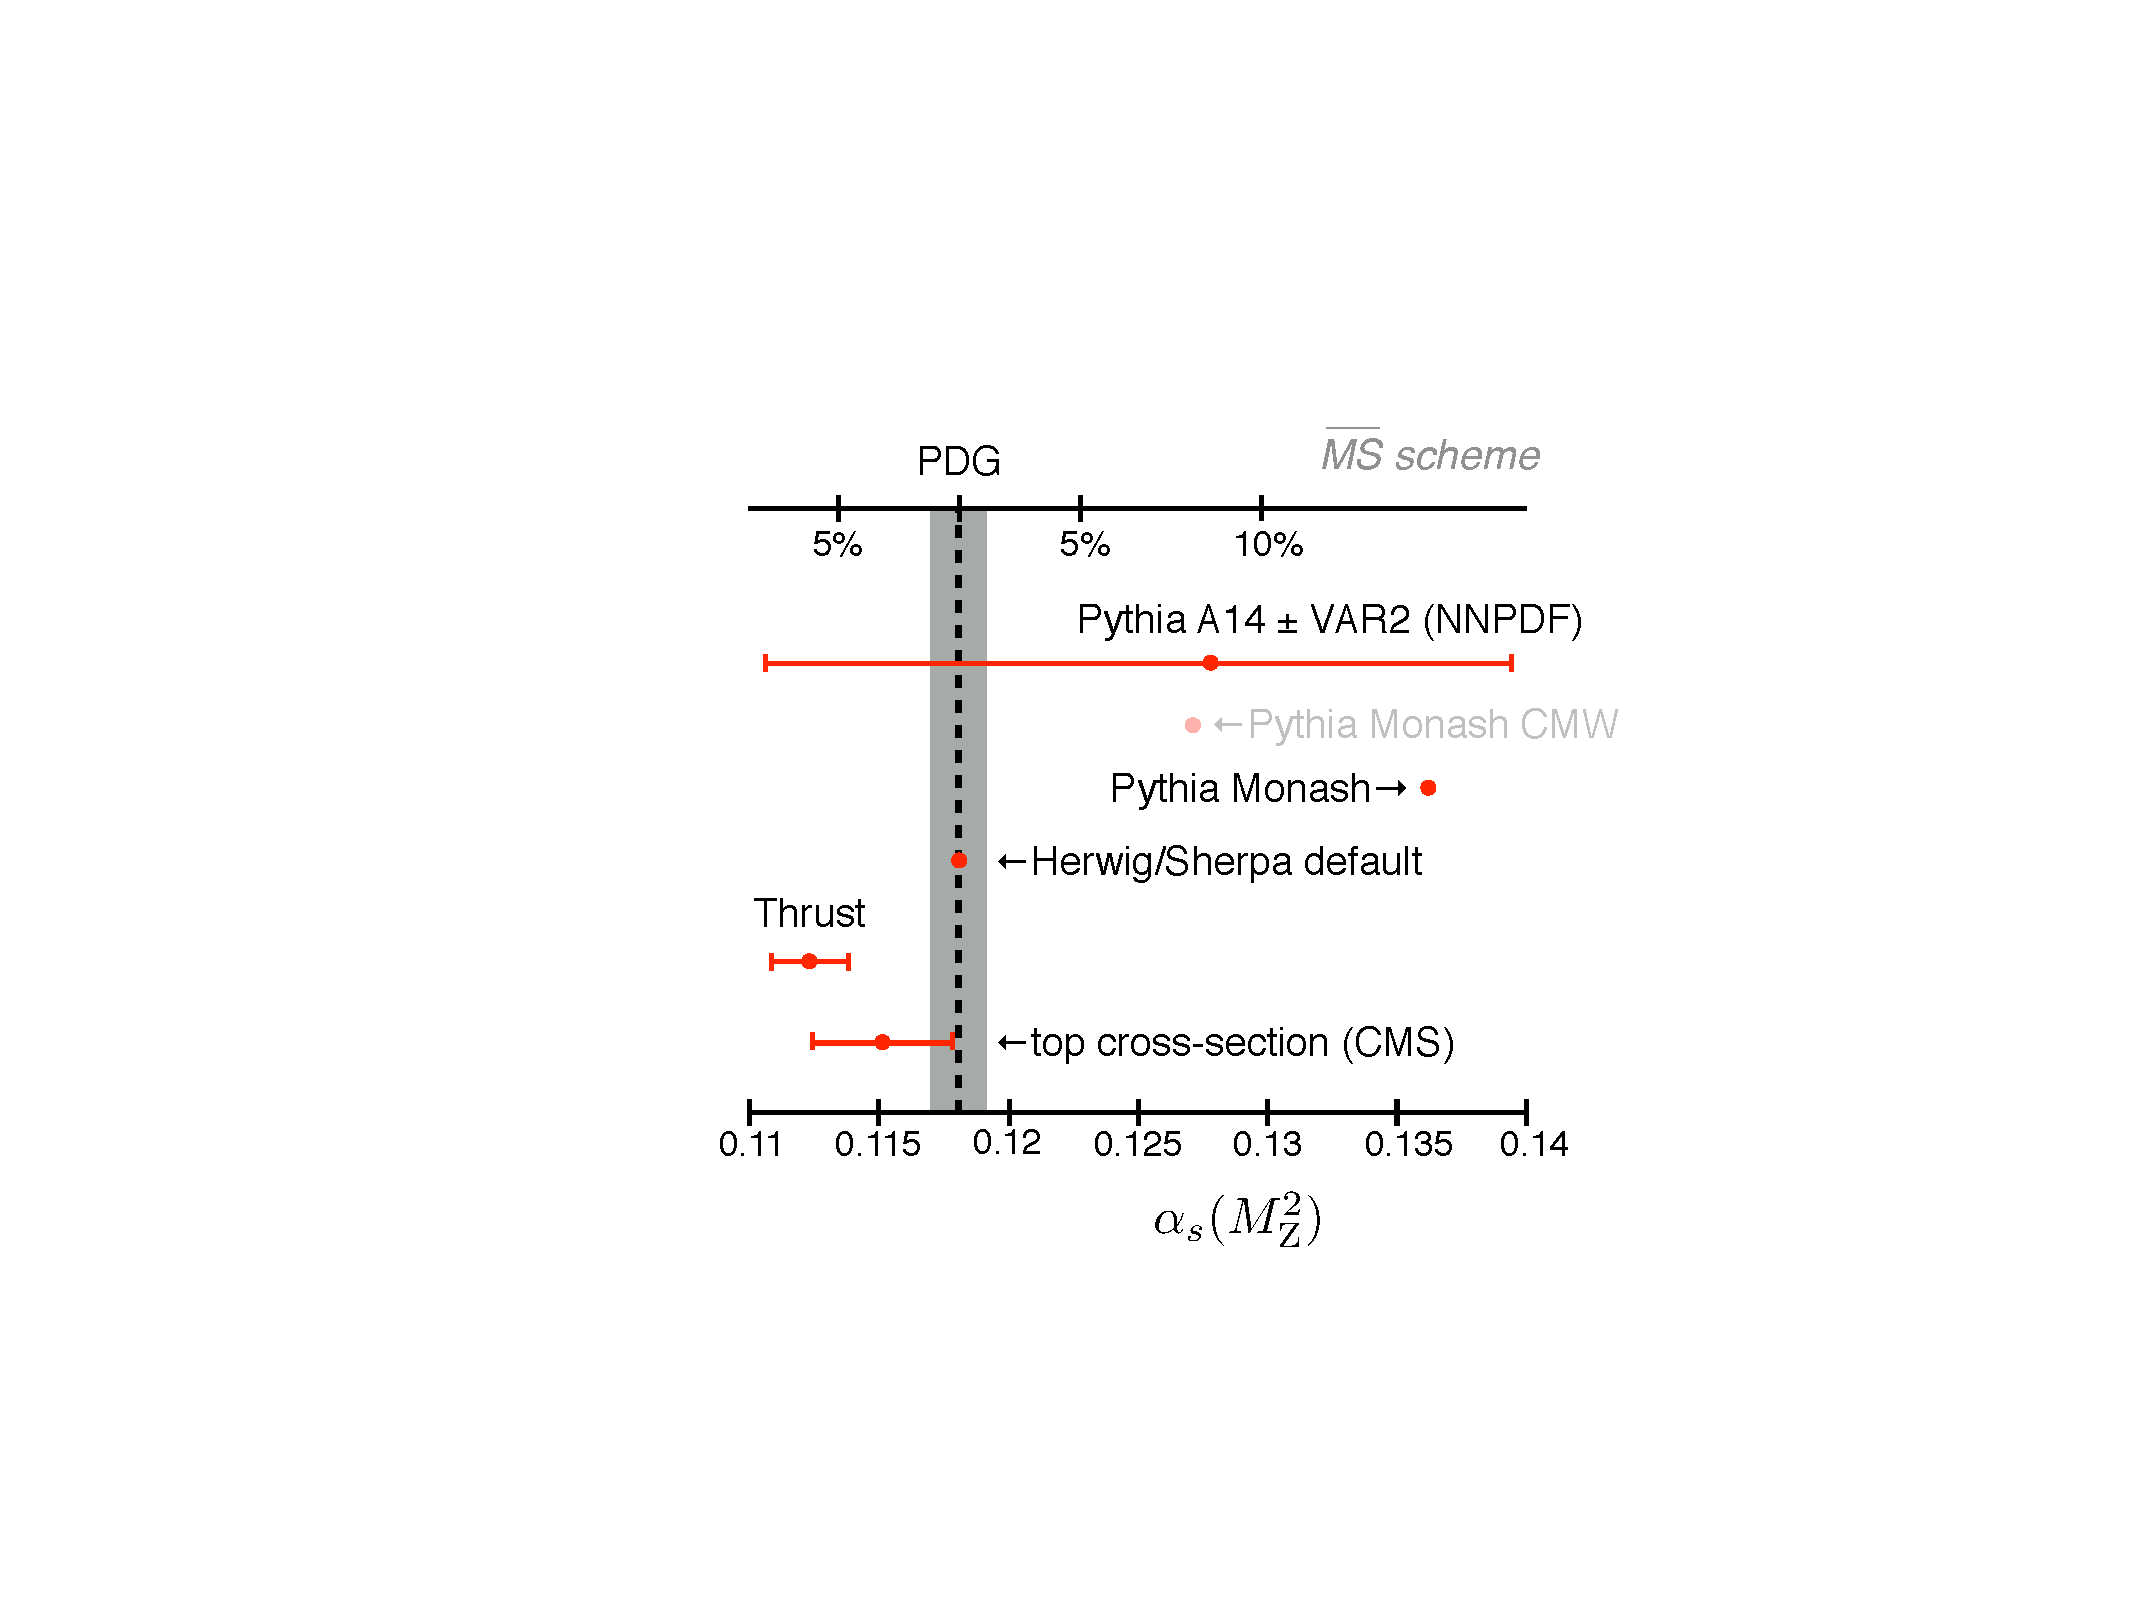
\includegraphics[width = 0.6\columnwidth]{jetsub_alphas_alphas_propaganda.pdf}
\end{center}
\caption{Various values of $\alpha_s$ in the $\overline{\mathrm{MS}}$ scheme, including the world-average shown as a black dashed line with a grey uncertainty band~\cite{Olive:2016xmw}.
%
The point labeled \textit{Thrust} is from LEP data~\cite{Abbate:2010xh,Hoang:2015hka,Heister:2003aj,Abdallah:2004xe,Abreu:1996mk,Abreu:1999rc,Biebel:1999zt,Adeva:1992gv,Abbiendi:2004qz,Abe:1994mf}.
%
The measurement using the CMS top cross-section measurement is the first NNLO extraction at the LHC~\cite{Chatrchyan:2013haa}.
%
The other points are the $\alpha_s$ parameter value used in the final state shower in various PS generaters: \textsc{Herwig~7}~\cite{Bellm:2015jjp} and \textsc{Sherpa}~\cite{Gleisberg:2008ta} use the world-average by default, while \textsc{Pythia~8}~\cite{Sjostrand:2006za,Sjostrand:2014zea} employs a higher value in both the Monash default tune~\cite{Skands:2014pea} and the A14 tunes (with VAR2 as an A14 uncertainty variation)~\cite{ATL-PHYS-PUB-2014-021}.
%
The order at which $\alpha_s$ is utilized is not the same in all cases.}
\label{jetsub_alphas_jetsub_alphas_fig:propaganda}
\end{figure}


Extractions based on $e^+e^-$ event shapes are sensitive to soft and collinear regions of phase space, which are modeled with precision
using higher-order resummation.
%
Figure~\cite{jetsub_alphas_jetsub_alphas_fig:propaganda} shows various values of $\alpha_s$ extracted with next-to-next-to-leading order (NNLO) calculations including various levels of resummation, such as next-to-next-to-next-to-leading logarithmic (N$^3$LL) for the thrust-based extraction.
%
Also shown are the values of $\alpha_s$ used as inputs to various Parton Shower (PS) generators.%
\footnote{Note that these programs implement much more than just the QCD parton shower.  For example, radiated photons are also generated, though the impact of those electroweak processes is quite negligible here (as opposed to photons from $\pi^0\rightarrow\gamma\gamma$).}
%
The value of $\alpha_s$ in the final-state PS is also sensitive to the soft and collinear regime of QCD (albeit in different ways); interestingly, the values used in the \textsc{Pythia~8} program~\cite{Sjostrand:2006za,Sjostrand:2007gs}, which are fit to $e^+e^-$ event shape data, suggest a higher value of $\alpha_s$ than the lattice result by about 15\%.
%
Another challenge with the event-shape extraction is that non-perturbative (NP) corrections are nearly degenerate with changes to $\alpha_s$ \cite{Abbate:2010xh}.
%
This is in part because techniques to parametrically separate NP effects from perturbative effects (i.e.~jet grooming techniques to be discussed below) were not mature at the time of the Large Electron Positron (LEP) collider, and because the energy scale at LEP did not allow for a large lever-arm between energy scales.
%
The sensitivity to low-energy scales where QCD is in the NP regime is also a key challenge for the lattice determination.
%
It would therefore be timely for a precision extraction of $\alpha_s$ using jets at the LHC.

For most analyses at the LHC so far, jets have been used mainly as proxies for quark and gluon four-vectors.
%
The multiplicity and kinematics of jets in purely hadronic final states can be predicted to high $\alpha_s$ orders in perturbation theory with e.g.\ NNLOJET~\cite{Currie:2016bfm,Currie:2017ctp} and NLOJet++~\cite{Nagy:2001fj,Nagy:2003tz}.
%
As a result, measurements of jet multiplicities, energies, and angles can be used to extract $\alpha_s$~\cite{ATLAS:2015yaa,Aaboud:2017fml,Khachatryan:2014waa,CMS:2014mna,Chatrchyan:2013txa}.
%
Even though these measurements have achieved an uncertainty of around $5\%$, they have not yet been included in the Particle Data Group (PDG) combination~\cite{Olive:2016xmw} since they are using only next-to-leading-order (NLO) theory calculations.
%
With recent progress in higher-order calculations, this will likely change soon, and it is noteworthy that an extraction using the recent NNLO $t\bar{t}$ cross-section \cite{Czakon:2013goa} is now included (see Fig.~\ref{jetsub_alphas_jetsub_alphas_fig:propaganda}).

In extractions based on fixed-order perturbation theory, the collinear region defining the internal
structure of jets is avoided in part due to the lack of precision calculations.%
\footnote{Logarithms of the jet radius $R$ may be important when the jet radius is small, and there are techniques to incorporate these corrections into fixed-order calculations~\cite{Dasgupta:2016bnd,Dasgupta:2014yra}.}
%
It is important to remember that jets are not in one-to-one correspondence with individual quarks and gluons, but rather to clusters of quarks and gluons; for this reason, the substructure of jets is also governed by $\alpha_s$.
%
Recent theoretical and experimental advances in jet substructure have shown that the radiation pattern inside jets has great physics potential~\cite{Abdesselam:2010pt,Altheimer:2012mn,Altheimer:2013yza,Adams:2015hiv,Larkoski:2017jix}.
%
To date, the focus of jet substructures studies has been mostly on tagging the origin of jets and searching for physics beyond the Standard Model.
%
However, present and future precision may be sufficient to make a useful measurement of $\alpha_s$.

A key tool to facilitate a substructure extraction of $\alpha_s$ are jet grooming techniques, which systematically removes soft and wide-angle radiation from jets \cite{Butterworth:2008iy,Ellis:2009su,Ellis:2009me,Krohn:2009th,Dasgupta:2013ihk,Larkoski:2014wba}.
%
Jet grooming can parametrically separate the NP radiation in the jet from the hard perturbatively-described components.
%
At a hadron collider, grooming also mitigates the contribution from the underlying event and additional nearly simultaneous interactions (pileup).
%
Theoretical calculations for groomed observables have been performed at NLL~\cite{Marzani:2017kqd,Marzani:2017mva} and NNLL~\cite{Frye:2016aiz,Frye:2016okc} accuracy and will be extended to higher orders as calculations become available.
%
Recently, ATLAS~\cite{Aaboud:2017qwh} and CMS~\cite{CMS-PAS-SMP-16-010} demonstrated 5-10\% measurement uncertainties of these calculated quantities using existing technologies.

The purpose of this paper is to study the feasibility of a measurement of $\alpha_s$ using jet substructure at the LHC, using jet shapes that are infrared and collinear (IRC) safe.
%
Similar techniques would of course also be interesting at both a low- and high-energy $e^+e^-$ collider; we focus here on $pp$ since high-quality data are now pouring out of the LHC.
%
We view this work as part of a broader program to apply jet grooming techniques for precision QCD (see also \cite{Hoang:2017kmk} for
applications to the top quark mass).
%
There are significant experimental and theoretical challenges to achieve success in this program, but we believe it is possible with community synergy.
%
An $\alpha_s$ extraction represents a concrete goal to push the accuracy and understanding of jet substructure calculations in particular and QCD calculations more generally.

This remainder of this work is organized as follows.
%
In Sec.~\ref{jetsub_alphas_sec:definitions}, we define the observables and grooming strategies that will be considered in this paper.
%
In Sec.~\ref{jetsub_alphas_sec:softcomplications}, we highlight a number of theoretical and experimental benefits of jet grooming, which make groomed observables particularly interesting for extractions of $\alpha_s$.
%
In Sec.~\ref{jetsub_alphas_sec:jetmass}, we discuss the sensitivity of groomed jet mass to the value of $\alpha_s$ using both analytic expressions and PS generators.
%
In Sec.~\ref{jetsub_alphas_sec:ben_study}, an idealized setup is used to illustrate how an extraction of $\alpha_s$ might work at the LHC, using realistic estimates of both the theoretical and experimental uncertainties.
%
We conclude in Sec.~\ref{jetsub_alphas_sec:future} and discuss future directions for improving both the theoretical and experimental uncertainties for $\alpha_s$ extractions from jet substructure.

\section{Observable and Algorithm Definitions}
\label{jetsub_alphas_sec:definitions}

In this section, we briefly review the definitions of the observables and grooming procedures that we will focus on in this paper.

%%%%%%%%%%%%%%%%%%%%%%%%%%%%%%%%%%%%%%%
\subsection{Two-point Correlators}\label{jetsub_alphas_sec:shape_def}
%%%%%%%%%%%%%%%%%%%%%%%%%%%%%%%%%%%%%%%

A simple class of jet shape observables that have sensitivity to the value of $\alpha_s$ are two-point correlation functions~\cite{Banfi:2004yd,Larkoski:2013eya}.
%
There has been significant theoretical study of these objects, and their perturbative behavior is understood to relatively high accuracy.
%
For a set of constituents $\{i\}$ in a jet $J$, the two-point correlation functions in $pp$ collisions are defined as
%
\begin{equation}
\label{jetsub_alphas_eq:ppe2}
\left.e_2^{(\alpha)}\right|_{pp}=\frac{1}{p_{TJ}^2}\sum_{i<j\in J} p_{Ti} \, p_{Tj} \, \left(\frac{R_{ij}}{R}\right)^\alpha\,, 
\end{equation}
where $p_{Ti}$ is the transverse momentum of particle $i$ with respect to the beam axis, $p_{TJ}$ is the transverse momentum of the jet, $R_{ij}$ is the distance between particles $i$ and $j$ in the rapidity-azimuthal angle plane, and $R$ is the jet radius.
%
Note that some authors define the correlation functions without the $R^\alpha$ factor in the denominator.
%
The angular exponent $\alpha$ is a parameter that controls the sensitivity to wide-angle emissions.
%
If all emissions in the jet are nearly collinear, then the two-point energy correlation function reduces to a function of the jet mass ($m$) when $\alpha=2$:
\begin{equation}
e_2^{(2)}\sim \frac{m^2}{R^2\, p_{T}^2}\,.
\end{equation} 

In this paper, we primarily restrict ourselves to the case of $\alpha=2$ as this has been the focus so far from both the theoretical~\cite{Frye:2016okc,Frye:2016aiz,Marzani:2017kqd,Marzani:2017mva} and experimental~\cite{Aaboud:2017qwh,CMS-PAS-SMP-16-010} communities.
%
However, it is interesting to study if other values of $\alpha$ could provide improved sensitivity to $\alpha_s$.
%
Another benchmark value is $\alpha=1$, which corresponds to $k_T$ (or broadening) instead of mass.
%
The two-point correlation functions are closely related to the jet angularities~\cite{Berger:2003iw,Almeida:2008yp,Ellis:2010rwa,Larkoski:2014pca}, with the latter being defined with respect to a jet axis.

%%%%%%%%%%%%%%%%%%%%%%%%%%%%%%%%%%%%%%%
\subsection{Grooming Techniques}\label{jetsub_alphas_sec:groom_tech}
%%%%%%%%%%%%%%%%%%%%%%%%%%%%%%%%%%%%%%%

There are a variety of jet grooming techniques to mitigate soft and wide-angle jet contamination~\cite{Butterworth:2008iy,Ellis:2009su,Ellis:2009me,Krohn:2009th,Dasgupta:2013ihk,Larkoski:2014wba}.
%
We focus here on the Soft Drop algorithm~\cite{Larkoski:2014wba}, defined using Cambridge/Aachen (C/A) reclustering \cite{Dokshitzer:1997in,Wobisch:1998wt,Wobisch:2000dk}.
%
Starting from a jet identified with an IRC-safe jet algorithm (such as anti-$k_t$ \cite{Cacciari:2008gp}), Soft Drop proceeds as follow:
%
\begin{enumerate}
%
\item Recluster the jet using the C/A clustering algorithm, producing an angular-ordered branching history for the jet.
%
\item Step through the branching history of the reclustered jet.  At each step, check the Soft Drop condition
%
\begin{equation}\label{jetsub_alphas_eq:sd_cut}
\frac{\min\left[ p_{Ti}, p_{Tj}  \right]}{p_{Ti}+p_{Tj}}> z_{\mathrm{cut}} \left(   \frac{R_{ij}}{R}\right)^\beta \,,
\end{equation}
%
where $z_{\mathrm{cut}} $ is a parameter defining the scale below which soft radiation is removed, and $\beta$ is an exponent that controls the angular scale for removal.
%
If the Soft Drop condition is not satisfied, then the softer of the two branches is removed from the jet.  This process is then iterated on the harder branch.
%
\item The Soft Drop procedure terminates once the Soft Drop condition is satisfied.
%
\end{enumerate}
%
This procedure generalizes the modified Mass Drop Tagger (mMDT)~\cite{Dasgupta:2013ihk}, which corresponds to $\beta=0$ in the Soft Drop procedure described above.
%
Note that non-global logarithms~\cite{Dasgupta:2001sh} are formally removed from the soft drop mass distribution, even when $\beta>0$ (though clearly they are restored as $\beta\rightarrow\infty$).

\section{Grooming Away Soft Complications}
\label{jetsub_alphas_sec:softcomplications}

Having defined the observables and grooming procedures of interest, in this section we provide a general discussion of the potential advantages of using groomed jet observables for extractions of $\alpha_s$.
%
The grooming procedure significantly simplifies a number of theoretical and experimental issues related to precision calculations and measurements in a $pp$ environment.
%
In particular, grooming provides:
%
\begin{itemize}
\item Mitigation of NP effects;
\item Perturbative simplicity; and
\item Improved detector resolution, due in large part to a reduced pileup sensitivity.
\end{itemize}
%
Each of these will be discussed in more detail below.
%
Combined, we believe that they provide a strong motivation for the measurement of  groomed jet observables, and the possibility of performing a precision extraction of $\alpha_s$ using jet substructure at the LHC.

%%%%%%%%%%%%%%%%%%%%%%%%%%%%%%%%%%%%%
\subsection{Mitigating Non-perturbative Effects}
%%%%%%%%%%%%%%%%%%%%%%%%%%%%%%%%%%%%%

\begin{figure}[t]
\begin{center}
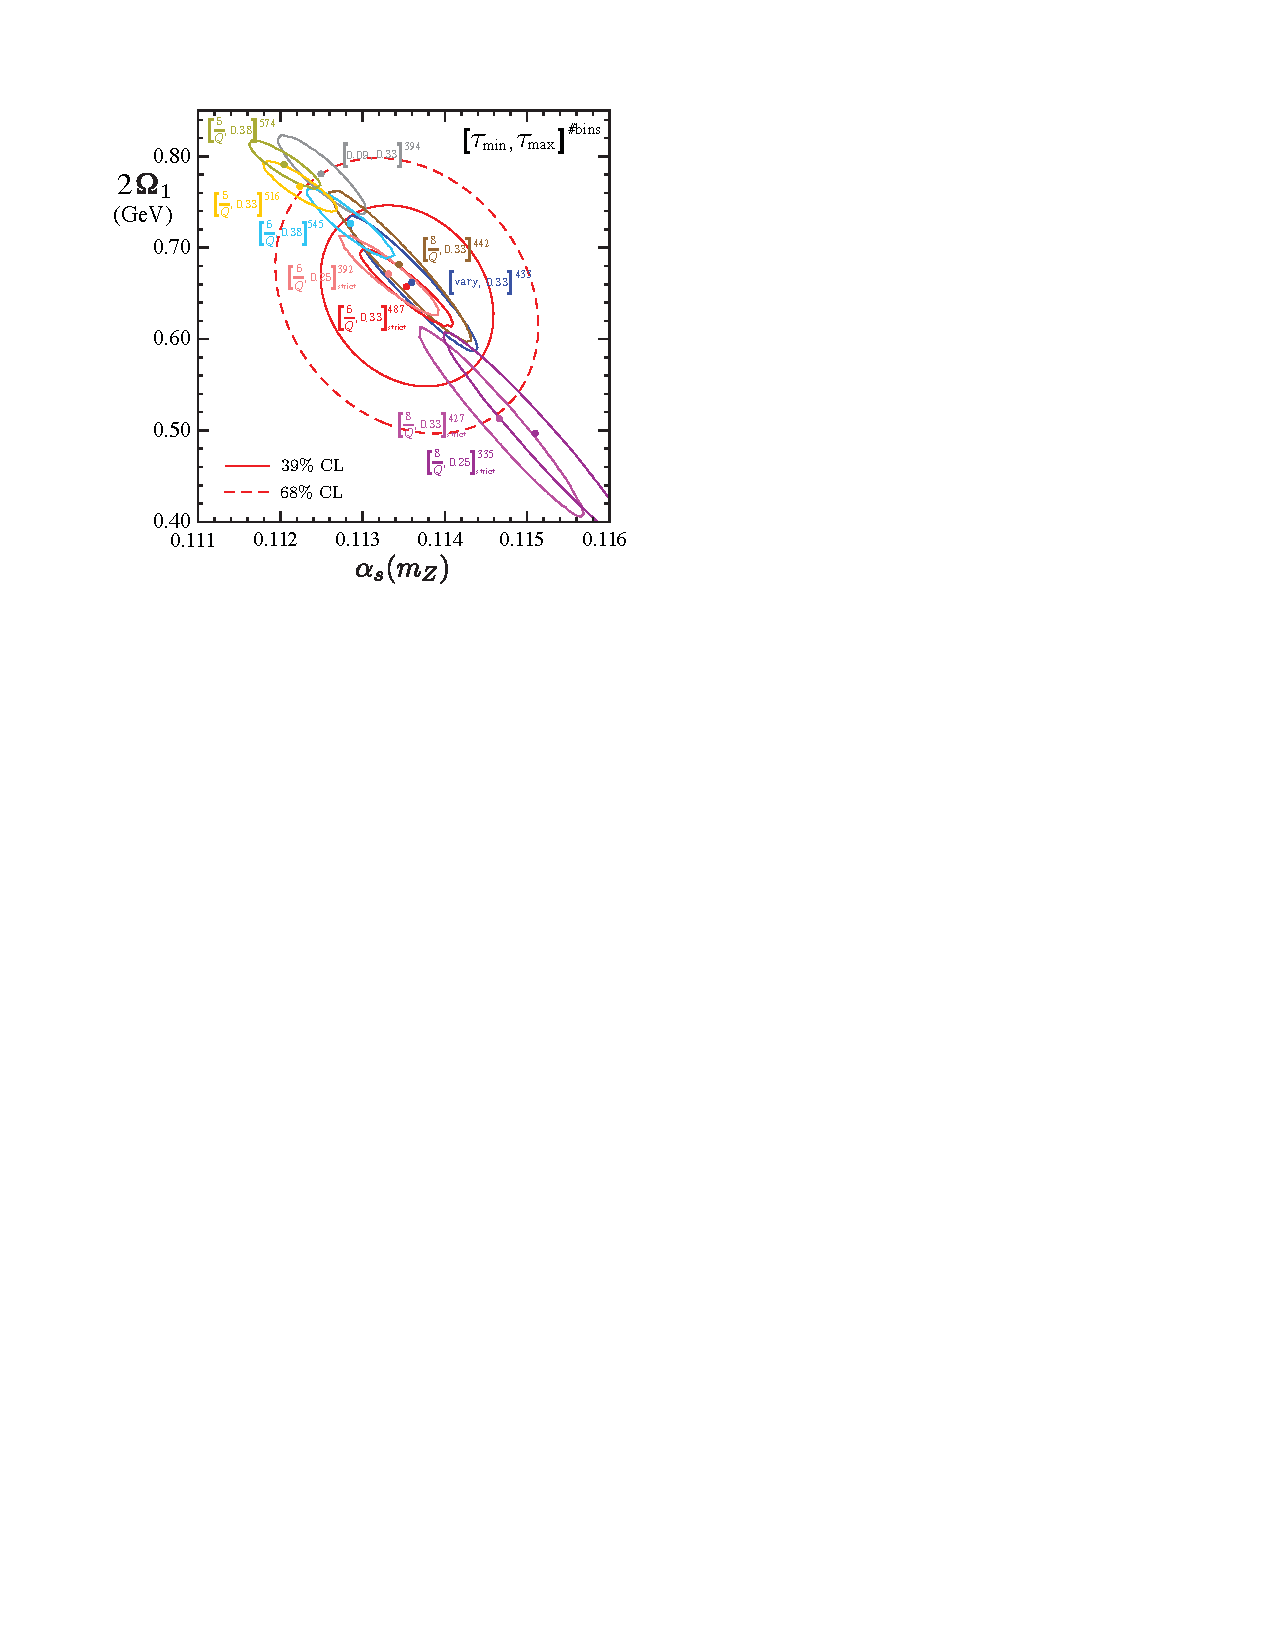
\includegraphics[width = 0.6\columnwidth]{jetsub_alphas_correlation_firstmoment.pdf}
\end{center}
\caption{An illustration of the correlations between the first NP moment $\Omega_1$ and $\alpha_s$ for the thrust observables.
%
NP effects for groomed observables have a significantly different structure, providing the possibility for complementary information to the extraction from (ungroomed) event shapes in $e^+e^-$.
%
Figure from Ref.~\cite{Abbate:2010xh}.}
\label{jetsub_alphas_fig:correlation_firstmoment}
\end{figure}

One of the primary complications of $\alpha_s$ extractions using event shapes is NP corrections, which cannot currently be calculated from first principles.
%
Since event shape observables probe singular regions of the phase space, they are necessarily sensitive to NP corrections.  
%
For $e^+e^-$ dijet event shapes, such as thrust, these NP corrections can be given operator definitions in the dijet limit.
%
Although these operators cannot be calculated, they can be modeled using \textit{shape functions}~\cite{Korchemsky:1999kt,Korchemsky:2000kp,Hoang:2007vb,Ligeti:2008ac}.%
\footnote{There are other approaches to analytically describe and fit NP effects that have similar features to shape functions.  Another example is the dispersive model~\cite{Dokshitzer:1995qm,Dokshitzer:1995zt} which has also been used to make extractions of $\alpha_s$ using $e^+e^-$ event shapes~\cite{Gehrmann:2012sc}.}
%
These shape functions can be systematically expanded in moments, and for moderately large values of the observable, only the first moment ($\Omega_1$) is required.
%
This moment can be shown to be universal for a wide range of observables \cite{Lee:2006fn,Lee:2007jr}, and can therefore be extracted from data along with $\alpha_s$~\cite{Abbate:2010xh,Abbate:2012jh,Hoang:2015hka}.\footnote{See Ref.~\cite{Salam:2001bd,Mateu:2012nk} for subtleties related to hadron masses and the breakdown of universality.}
%
This moment, however, is highly correlated with $\alpha_s$ as shown in Fig.~\ref{jetsub_alphas_fig:correlation_firstmoment}.
%
Therefore, observables with different, and preferably suppressed, NP effects could provide valuable complementary information for $\alpha_s$ extractions.
%

Using a scaling argument, it is a straightforward exercise to compute the value of the groomed two-point correlators at which NP effects are expected to be important.
%
This was considered in Ref.~\cite{Frye:2016aiz,Dasgupta:2013ihk} where it was shown that NP effects become important when (for $\alpha \geq 1$),
%
\begin{equation}
\label{jetsub_alphas_eq:np}
\left. e_2^{(\alpha)}\right |_{\mathrm{NP}} \simeq  \left( \frac{\Lambda_{\mathrm{QCD}}}{z_{\mathrm{cut}}  Q}  \right)^{\frac{\alpha-1}{1+\beta}}  \frac{\Lambda_{\mathrm{QCD}}}{Q}\,,
\end{equation}
%
where $Q=p_TR$ is the starting scale of jet fragmentation.
%
When $\alpha< 1$, the value is instead $(\Lambda_{\mathrm{QCD}}/(p_TR))^\alpha$.
%
If we consider for concreteness the jet mass ($\alpha=2$) we can learn a number of interesting lessons.
%
First, by taking $\beta\to \infty$, we obtain the ungroomed result
%
\begin{equation}
\left. e_2^{(2)} \right |_{\mathrm{NP}} \simeq  \frac{\Lambda_{\mathrm{QCD}}}{p_TR}\,,
\end{equation} 
%
while the groomed result gives 
%
\begin{equation}
\left. e_2^{(2)} \right |_{\mathrm{NP}} \simeq  \left( \frac{\Lambda_{\mathrm{QCD}}}{z_{\mathrm{cut}}  p_TR}  \right)^{\frac{1}{1+\beta}}  \frac{\Lambda_{\mathrm{QCD}}}{p_TR}\,.
\end{equation}
%
For $z_{\mathrm{cut}}  p_T R \gg \Lambda_{\mathrm{QCD}}$, we see that the grooming significantly suppresses the scale of the NP physics, extending the range of perturbative validity by a factor of $({\Lambda_{\mathrm{QCD}}} / {z_{\mathrm{cut}}  p_TR})^{1/(1+\beta)}$.
%
For a $1$ TeV jet with $z_{\mathrm{cut}}  =0.1$ and $\beta=0$, this is an extension by a factor of $\sim 100$.
%
Furthermore, we observe that, under the assumption that $\beta \geq 0$, this suppression is maximized for $\beta=0$, motivating this choice in later studies.%
\footnote{Negative values of $\beta$ are also possible and could be interesting to study.  However, one would need to dedicate specific attention in the vicinity of the endpoint of the distribution, which is $e_2^{(\alpha)}=z_{\mathrm{cut}}^{-\alpha\beta}$ at LL.}

%
It is important to emphasize that just because the value of the mass at which NP physics enters is suppressed, this does not by itself imply that there is a larger region over which one has perturbative control.
%
In principle the whole distribution could be shifted to lower values.
%
We know, however, that for $e_2^{(2)}\geq z_{\mathrm{cut}} $, the distribution is parametrically unaffected by the grooming procedure, and is therefore identical to the ungroomed jet mass. 


\begin{figure}[t]
\begin{center}
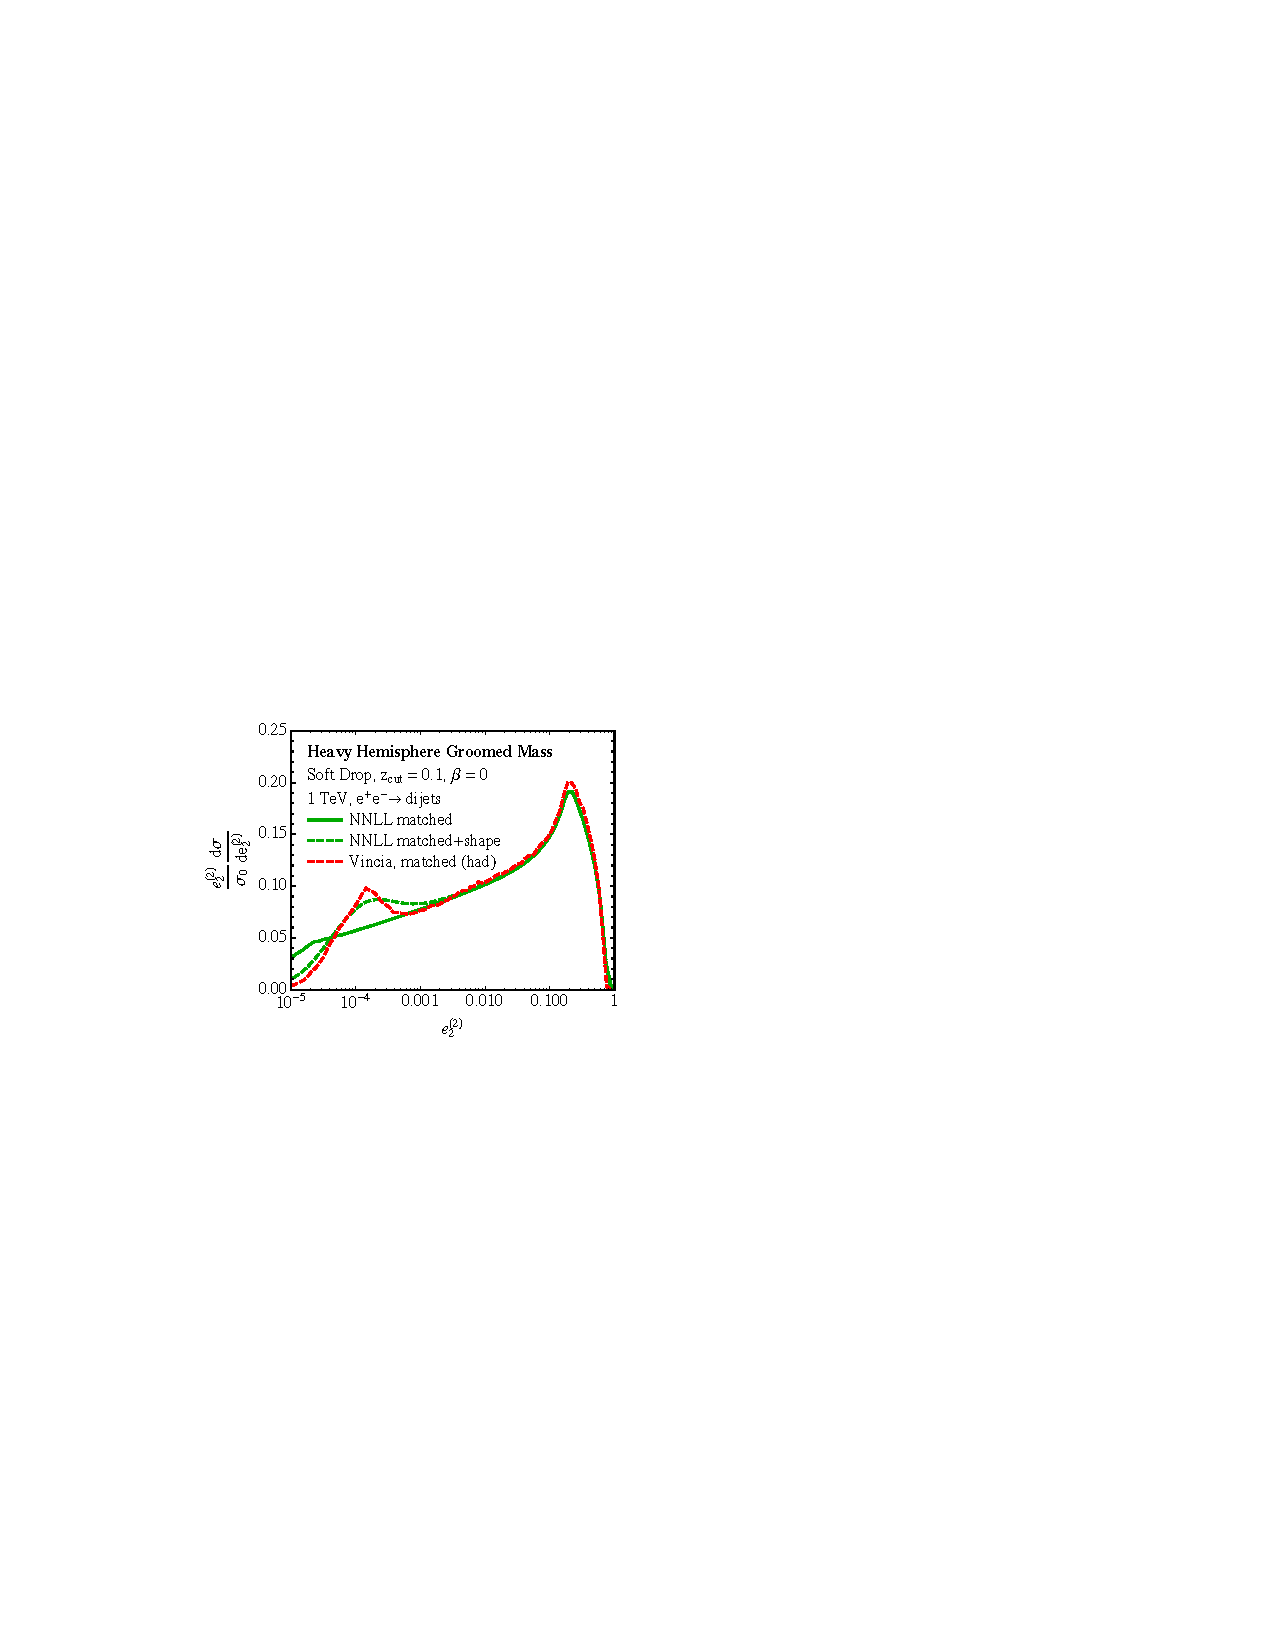
\includegraphics[width = 0.6\columnwidth]{jetsub_alphas_shape_function.pdf}
\end{center}
\caption{A plot showing the effects of NP corrections to the groomed jet mass. This illustrates first that the NP corrections are suppressed over a large range, and second that they take a very different form than for double-logarithmic observables. Figure from Ref.~\cite{Frye:2016aiz}.}
\label{jetsub_alphas_fig:shape_function}
\end{figure}

In addition to being suppressed, the structure of the NP corrections is quite different for groomed jet mass, which may provide complementary information compared to standard event shapes.
%
For event shape observables, NP corrections are typically large already at the Sudakov peak.
%
In the case of a groomed observable, since the NP corrections are suppressed and the observable is predominantly single logarithmic (exactly true when $\beta=0$), we instead see that the NP corrections appear as a bump on the falling distribution.
%
This is shown in Fig.~\ref{jetsub_alphas_fig:shape_function} along with a model using a shape function.
%
Due to the fact that this is a completely different behavior, it may have different correlations as compared with standard event shapes, though a more complete understanding of this effect is required. 

Finally, while we have so far focused on the effect of the grooming procedure on hadronization corrections and a comparison to $e^+e^-$ event shapes, we must also emphasize that the grooming plays an important role in suppressing NP corrections from the underlying event.
%
This is crucial for achieving a precision measurement in the $pp$ environment, since there is a limited theoretical understanding of the underlying event.
%
Here, we must rely purely on Monte Carlo model implementations of the underlying event.
%
Monte Carlo studies have shown that in the regime where one has perturbative control, underlying event is highly suppressed after mMDT/Soft Drop~\cite{Dasgupta:2013ihk,Larkoski:2014wba}.
%
This is again a significant benefit of groomed observables. 


%%%%%%%%%%%%%%%%%%%%%%%%%%%%%%%%%%%%%
\subsection{Perturbative Simplicity}
\label{jetsub_alphas_sec:pertsimplicity}
%%%%%%%%%%%%%%%%%%%%%%%%%%%%%%%%%%%%%

By studying the analytic behavior of grooming on the jet mass, the authors of Ref.~\cite{Dasgupta:2013ihk} showed that grooming could be designed to enhance the simplicity and calculability of various jet shapes.
%
In particular, grooming significantly simplifies the perturbative resummation in the $pp$ environment in addition to suppressing NP corrections.
%
Calculations of the standard jet mass in $pp$ typically suffer from the following two perturbative difficulties:
%
\begin{itemize}
%
\item Global color correlations, which complicate the structure of higher-order soft functions; and
%
\item Non-global logarithms \cite{Dasgupta:2001sh}, which complicate the perturbative structure for non-global measurements.
%
\end{itemize}
%
The jet mass was calculated in \cite{Jouttenus:2013hs} (\cite{arXiv:1207.1640}) for $H+$ jet with(out) a veto on additional radiation, supplemented with arguments that non-global effects are small.
%
These above two features highlight that the ungroomed jet mass depends significantly on the particular process that created the jet, significantly reducing its universality, and complicating its structure in a busy $pp$ environment.
%
By contrast, the use of grooming can make the jet mass nearly universal.

In Ref.~\cite{Frye:2016aiz}, it was shown that for $e_2^{(\alpha)}\ll z_{\mathrm{cut}}  \ll 1$, one can express the cross section for the groomed two-point correlator as
%
\begin{equation}
\label{jetsub_alphas_eq:fac_pp_e2}
\frac{d\sigma^{pp}}{de_2^{(\alpha)}}=\sum\limits_{k=q,\bar q, g}D_k(p_T^{\mathrm{min}}, y_\mathrm{max}, z_{\mathrm{cut}} , R) S_{C,k}(z_{\mathrm{cut}} , e_2^{(\alpha)})\otimes J_k (e_2^{(\alpha)})\,,
\end{equation}
%
where $S_{C,k}$ is the soft function and $J_k$ is the jet function.
%
The function $D_k$ depends on the parton flavor, and can be interpreted as the quark and gluon fractions.
%
While the quark and gluon fractions are generally not IRC-safe quantities, in this limit the quark fraction can be defined jet-by-jet as 
\begin{equation}
f_J=\sum\limits_{i\in J_{\mathrm{SD}}} f_i\,,
\end{equation}
with $f_q=1$, $f_{\bar q}=-1$, $f_g=0$, and $J_{\mathrm{SD}}$ are the parton-level constituents of the groomed jet.
%
The grooming procedure makes this definition IRC safe (see related jet flavor approach in Ref.~\cite{Banfi:2006hf}).
%
These fractions are independent of the value of the jet mass observable and can be extracted from fixed-order generators, for example MCFM \cite{Campbell:1999ah,Campbell:2010ff,Campbell:2011bn}.

The formula in Eq.~\ref{jetsub_alphas_eq:fac_pp_e2} has a number of remarkable consequences.
%
In the resummation region, we see that there are no non-global logarithms and there are no global color correlations.
%
The collinear soft and jet functions depend only on the jet flavor, so they are therefore identical to in the case of groomed jets in $e^+e^-$ collisions.
%
In the resummation region, the grooming algorithm has therefore allowed the jet to be isolated from its $pp$ environment, and the only required input from the hard scattering process are the quark and gluon fractions. 

It is important to emphasize that this simplification does not occur throughout the entire distribution.
%
In particular, it does not hold for $m \gg Qz_{\mathrm{cut}} $, though this is the fixed order region, where we can match to standard fixed order perturbation theory.
%
This matching has been performed to (N)NLO for dijets ($V$+jets) \cite{Frye:2016aiz,Marzani:2017kqd,Marzani:2017mva}.
%
Ideally this would be done using $2\to 3$ matrix elements at NNLO, which are just now becoming available~\cite{Gehrmann:2015bfy,Dunbar:2016aux,Badger:2013yda,Badger:2017jhb,Abreu:2017hqn}.

%%%%%%%%%%%%%%%%%%%%%%%%%%%%%%%%%%%%%
\subsection{Pileup Resilience}
%%%%%%%%%%%%%%%%%%%%%%%%%%%%%%%%%%%%%

Arguably the biggest experimental challenge for precision physics at a high luminosity $pp$ collider is noise from \textit{pileup}: multiple nearly simultaneous proton-proton collisions.
%
Jet shapes are particularly sensitive to pileup; for example, the jet mass scales as $\mathcal{O}(A^2)$~\cite{Salam:2009jx} for the jet catchment area $A$~\cite{Cacciari:2008gn} (whereas the jet $p_\mathrm{T}$ scales linearly with $A$).
%
The jet-area subtraction that works well for $p_\mathrm{T}$ has been extended to event shapes~\cite{Soyez:2012hv}, but must be re-calibrated per observable.
%
Constituent-based pileup subtraction schemes~\cite{Cacciari:2014gra,Krohn:2013lba,Bertolini:2014bba,Berta:2014eza,Komiske:2017ubm} show great promise and are actively being studied and adapted to the actual experimental settings~\cite{CMS-PAS-JME-14-001,CMS-DP-2015-034,ATLAS-CONF-2017-065,ATL-PHYS-PUB-2017-020,Aad:2015ina}.
%
Even without constituent-based subtraction techniques, though, there is a large reduction in pileup sensitivity to jet substructure from grooming~\cite{CMS-PAS-JME-14-001,Aad:2015rpa,Aad:2015ina,Altheimer:2013yza}.
%
Grooming systematically removes soft and wide-angle radiation, which is exactly the profile characteristic of pileup.
%
Even with extreme levels of pileup (up to 300 collisions), grooming can preserve the distribution of the jet mass distribution~\cite{JetSubstructureECFA2014}. 

Despite the power of grooming for pileup suppression, there is still a residual degradation of resolution with increased levels of pileup which makes precision jet substructure measurements challenging at high instantaneous luminosity.
%
Track-based observables are robust to pileup because their vertex of origin can be well-distinguished from pileup vertices.
%
Precision track-based substructure observables have been calculated~\cite{Krohn:2012fg,Waalewijn:2012sv,Chang:2013rca,Elder:2017bkd}, but typically require universal NP input.
%
It may be interesting to do a track- and jet-substructure-based extraction of $\alpha_s$, but this is left as a possibility for future work.

\section{Observable Sensitivity to $\alpha_s$}
\label{jetsub_alphas_sec:jetmass}

In this section, we study the sensitivity of the groomed jet mass to variations in the value of $\alpha_s$.
%
We begin with a discussion based on the analytic formulae at LL accuracy.
%
We then perform a PS study, highlighting the interplay between the sensitivity of different parts of the distribution to variations in the value of $\alpha_s$ and NP effects.
%
Finally, we discuss the issue of Casimir scaling and the related issue of using normalized versus unnormalized distributions.


%%%%%%%%%%%%%%%%%%%%%%%%%%%
\subsection{Analytic Understanding}
\label{jetsub_alphas_sec:analytic}
%%%%%%%%%%%%%%%%%%%%%%%%%%%

To get an understanding of the sensitivity of the groomed mass distribution both to the value of $\alpha_s$ as well as to the quark and gluon composition, it is enlightening to study the LL distribution.
%
Here, for simplicity, we consider only the leading logs in the observable, in the resummation region; complete expressions can be found in Ref.~\cite{Larkoski:2014wba,Frye:2016aiz,Marzani:2017kqd,Marzani:2017mva}.
%
For $\beta=0$, the LL result at fixed coupling for the cumulative distribution in the resummation region takes the schematic form
%
\begin{equation}
\Sigma(e_2^{(2)})=\exp\left[ - \frac{\alpha_s C_i}{\pi} \log(z_{\mathrm{cut}} ) \log (e_2^{(2)}) \right]\,.
\end{equation}
%
This highlights that for $\beta=0$, the groomed jet mass is a single-logarithmic observable, contrasting with the standard double-logarithmic behavior of plain jet mass.
%
Differentiating the cumulative distribution, we obtain the spectrum
%
\begin{equation}
\label{jetsub_alphas_eq:ecf_ll_dsitribution}
e_2^{(2)} \frac{d\sigma}{d e_2^{(2)}}=   - \frac{\alpha_s C_i}{\pi} \log(z_{\mathrm{cut}} )   \exp\left[ - \frac{\alpha_s C_i}{\pi}  \log(z_{\mathrm{cut}} ) \log (e_2^{(2)}) \right].
\end{equation}
%
Here, we immediately see several interesting consequences.
%
In the resummation region, the slope of the distribution when plotted against $\log e_2^{(2)}$ is set by the product $\alpha_s C_i$, where $C_i$ is the Casimir factor, namely $C_F = 4/3$ for quarks and $C_A = 3$ for gluons.
%
We therefore see that the groomed mass is indeed sensitive to the value of $\alpha_s$.
%
Due to the larger color charge of gluons, we expect that samples of pure gluon jets would have a significantly higher sensitivity to the value of $\alpha_s$; this expectation will be born out in our parton shower studies below.
%
Because $\alpha_s$ is always multiplied by a color factor, though, knowing the precise quark/gluon composition of a sample is essential, as discussed in Sec.~\ref{jetsub_alphas_sec:casimir}.
%
In practice, the parton shower studies and the analytic studies that follow (see Sec.~\ref{jetsub_alphas_sec:ben_study}) include higher order effects, such as subleading terms in the splitting functions, that violate Casimir scaling.

%%%%%%%%%%%%%%%%%%%%%%%%%%%
\subsection{Parton Shower Study}
%%%%%%%%%%%%%%%%%%%%%%%%%%%

From the point of view of fitting for $\alpha_s$, a good observable is one whose probability distribution changes significantly with variations in $\alpha_s$.
%
However, many observables that significantly change with $\alpha_s$ are also very sensitive to NP effects, such as the constituent multiplicity inside jets.
%
Here, we study many two-point correlators to quantify the tradeoff between the sensitivity to $\alpha_s$ and the robustness to NP effects.

\begin{figure}[t]
\begin{center}
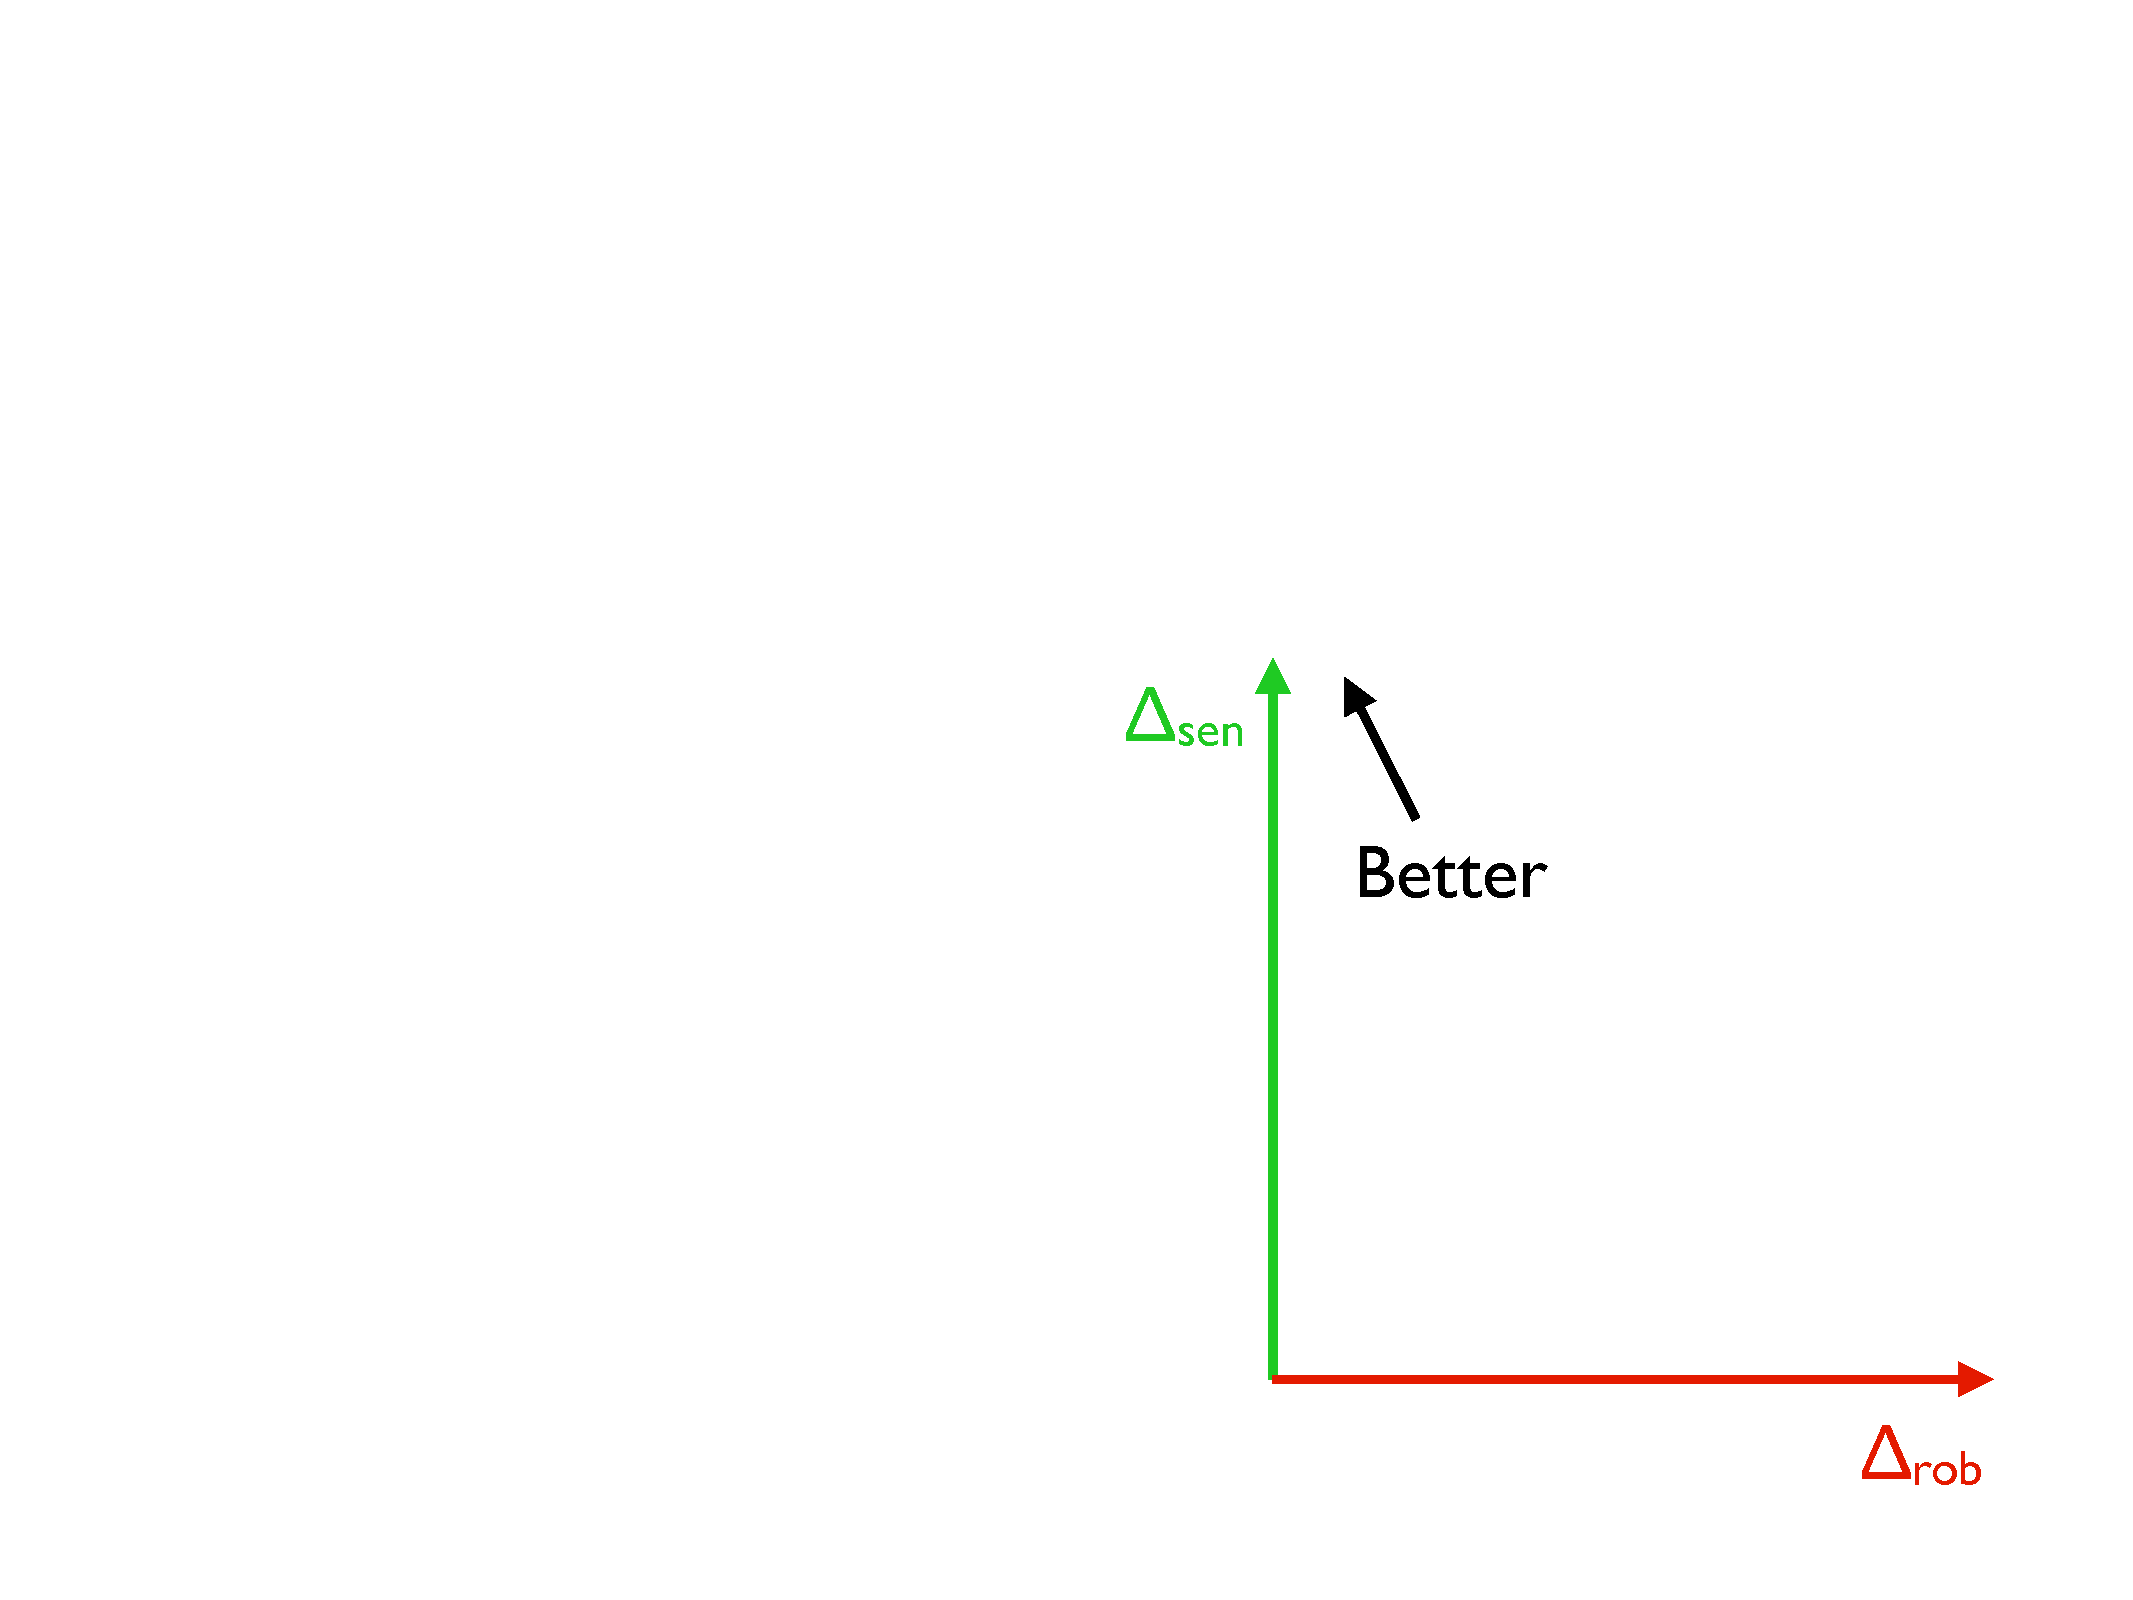
\includegraphics[width = 0.4\columnwidth]{jetsub_alphas_robustnessschematic.pdf}
\end{center}
\caption{A schematic diagram to illustrate the sensitivity-robustness plane defined by the separation power in Eq.~\ref{jetsub_alphas_eq:seppower}.}
\label{jetsub_alphas_fig:robustnessschematic}
\end{figure}

Given two probability distributions $f$ and $g$ in some observable $\lambda$, we define the separation power $\Delta(f,g)$~\cite{Harrison:1998yr} as
%
\begin{equation}
\label{jetsub_alphas_eq:seppower}
\Delta(f,g)=\frac{1}{2}\int d\lambda \, \frac{(f(\lambda)-g(\lambda))^2}{f(\lambda)+g(\lambda)}.
\end{equation}
%
The separation power is a number in $[0,1]$, where $\Delta=0$ if and only if $f=g$.
%
If $f$ is the nominal probability distribution of some observable and $g$ is the distribution of the same observable with a different value of $\alpha_s$, we would like $\Delta(f,g)$ close to 1 (sensitivity).
%
In contrast, if $g$ is the same as $f$ with some variation in the NP effects, then we would like $\Delta(f,g)$ to be close to $0$ (robustness).
%
The plane used to study the tradeoff between sensitivity and robustness is shown in Fig.~\ref{jetsub_alphas_fig:robustnessschematic}.
%
Not all information about $\alpha_s$ sensitivity is captured by a single point in Fig.~\ref{jetsub_alphas_fig:robustnessschematic}, because sensitivity to NP effects could be in regions of low $\alpha_s$ sensitivity and vice versa.
%
Therefore, it is also useful to study the integrand of Eq.~\ref{jetsub_alphas_eq:seppower} as a function of different observables $\lambda$.


This sensitivity-robustness tradeoff is studied using two parton shower generators: \textsc{Herwig~7}.1~\cite{Bellm:2015jjp,Reichelt:2017hts} with the default tune and \textsc{Pythia~8}.223~\cite{Sjostrand:2006za,Sjostrand:2014zea} with the tune Monash~\cite{Skands:2014pea}.  
%
These programs are formally LL accurate, though they include effects beyond Eq.~\ref{jetsub_alphas_eq:ecf_ll_dsitribution}.
%
Results are presented separately for quark and gluon jets, using the $Z+q$ and $Z+g$ hard-scattering processes.
%
We select jets with transverse momentum $p_\mathrm{T}>500$ GeV and rapidity $|y|<2.5$, clustered with the anti-$k_t$ algorithm~\cite{Cacciari:2008gp} algorithm using a jet radius $R=0.8$.
%
A variety of two-point correlators (as defined in Sec.~\ref{jetsub_alphas_sec:shape_def}) are studied, with $\alpha\in\{0.5,1.0, 2.0\}$ corresponding to the Les Houches Angularity~\cite{Gras:2017jty}, width, and mass, respectively. 
%
Additionally, various Soft Drop grooming parameters are studied by varying $\beta\in\{0,1,2\}$ and $z_\mathrm{cut}\in \{0.05,0.1,0.2\}$.  

\begin{figure}[t]
\begin{center}
\includegraphics[width = 0.49\columnwidth]{jetsub_alphas_sensitivity2a.pdf}\includegraphics[width = 0.48\columnwidth]{jetsub_alphas_sensitivity2b.pdf}
\end{center}
\caption{The sensitivity to $\alpha_s$ in \textsc{Herwig~7}.  Shown is the distribution of the normalized squared jet mass ($e_2^{(2)}$) for quark jets (left) and gluon jets (right), with higher values of the mass are on the left.  The blue line uses $\alpha_s=0.118$ while the green and orange lines have the value of $\alpha_s$ varied by $10\%$.  The lower panels show the ratio with respect to the $\alpha_s=0.118$ curve.}
\label{jetsub_alphas_fig:sensitivity}
\end{figure}

\begin{figure}[t]
\begin{center}
\includegraphics[width = 0.48\columnwidth]{jetsub_alphas_robustness2a.pdf}\includegraphics[width = 0.49\columnwidth]{jetsub_alphas_robustness2b.pdf}
\end{center}
\caption{The robustness to NP effects in \textsc{Herwig~7}, with the same distributions as Fig.~\ref{jetsub_alphas_fig:sensitivity}.
%
The blue line shows the default particle-level simulation that includes the standard cluster hadronization model.
%
The red curve has hadronization turned off and the green curve is the same as the blue, but with the \textsc{Herwig~7} model for multiple parton interactions (MPI) turned off.
%
MPI is also off for the red curve.}
\label{jetsub_alphas_fig:robustness}
\end{figure}

\begin{figure}[t]
\begin{center}
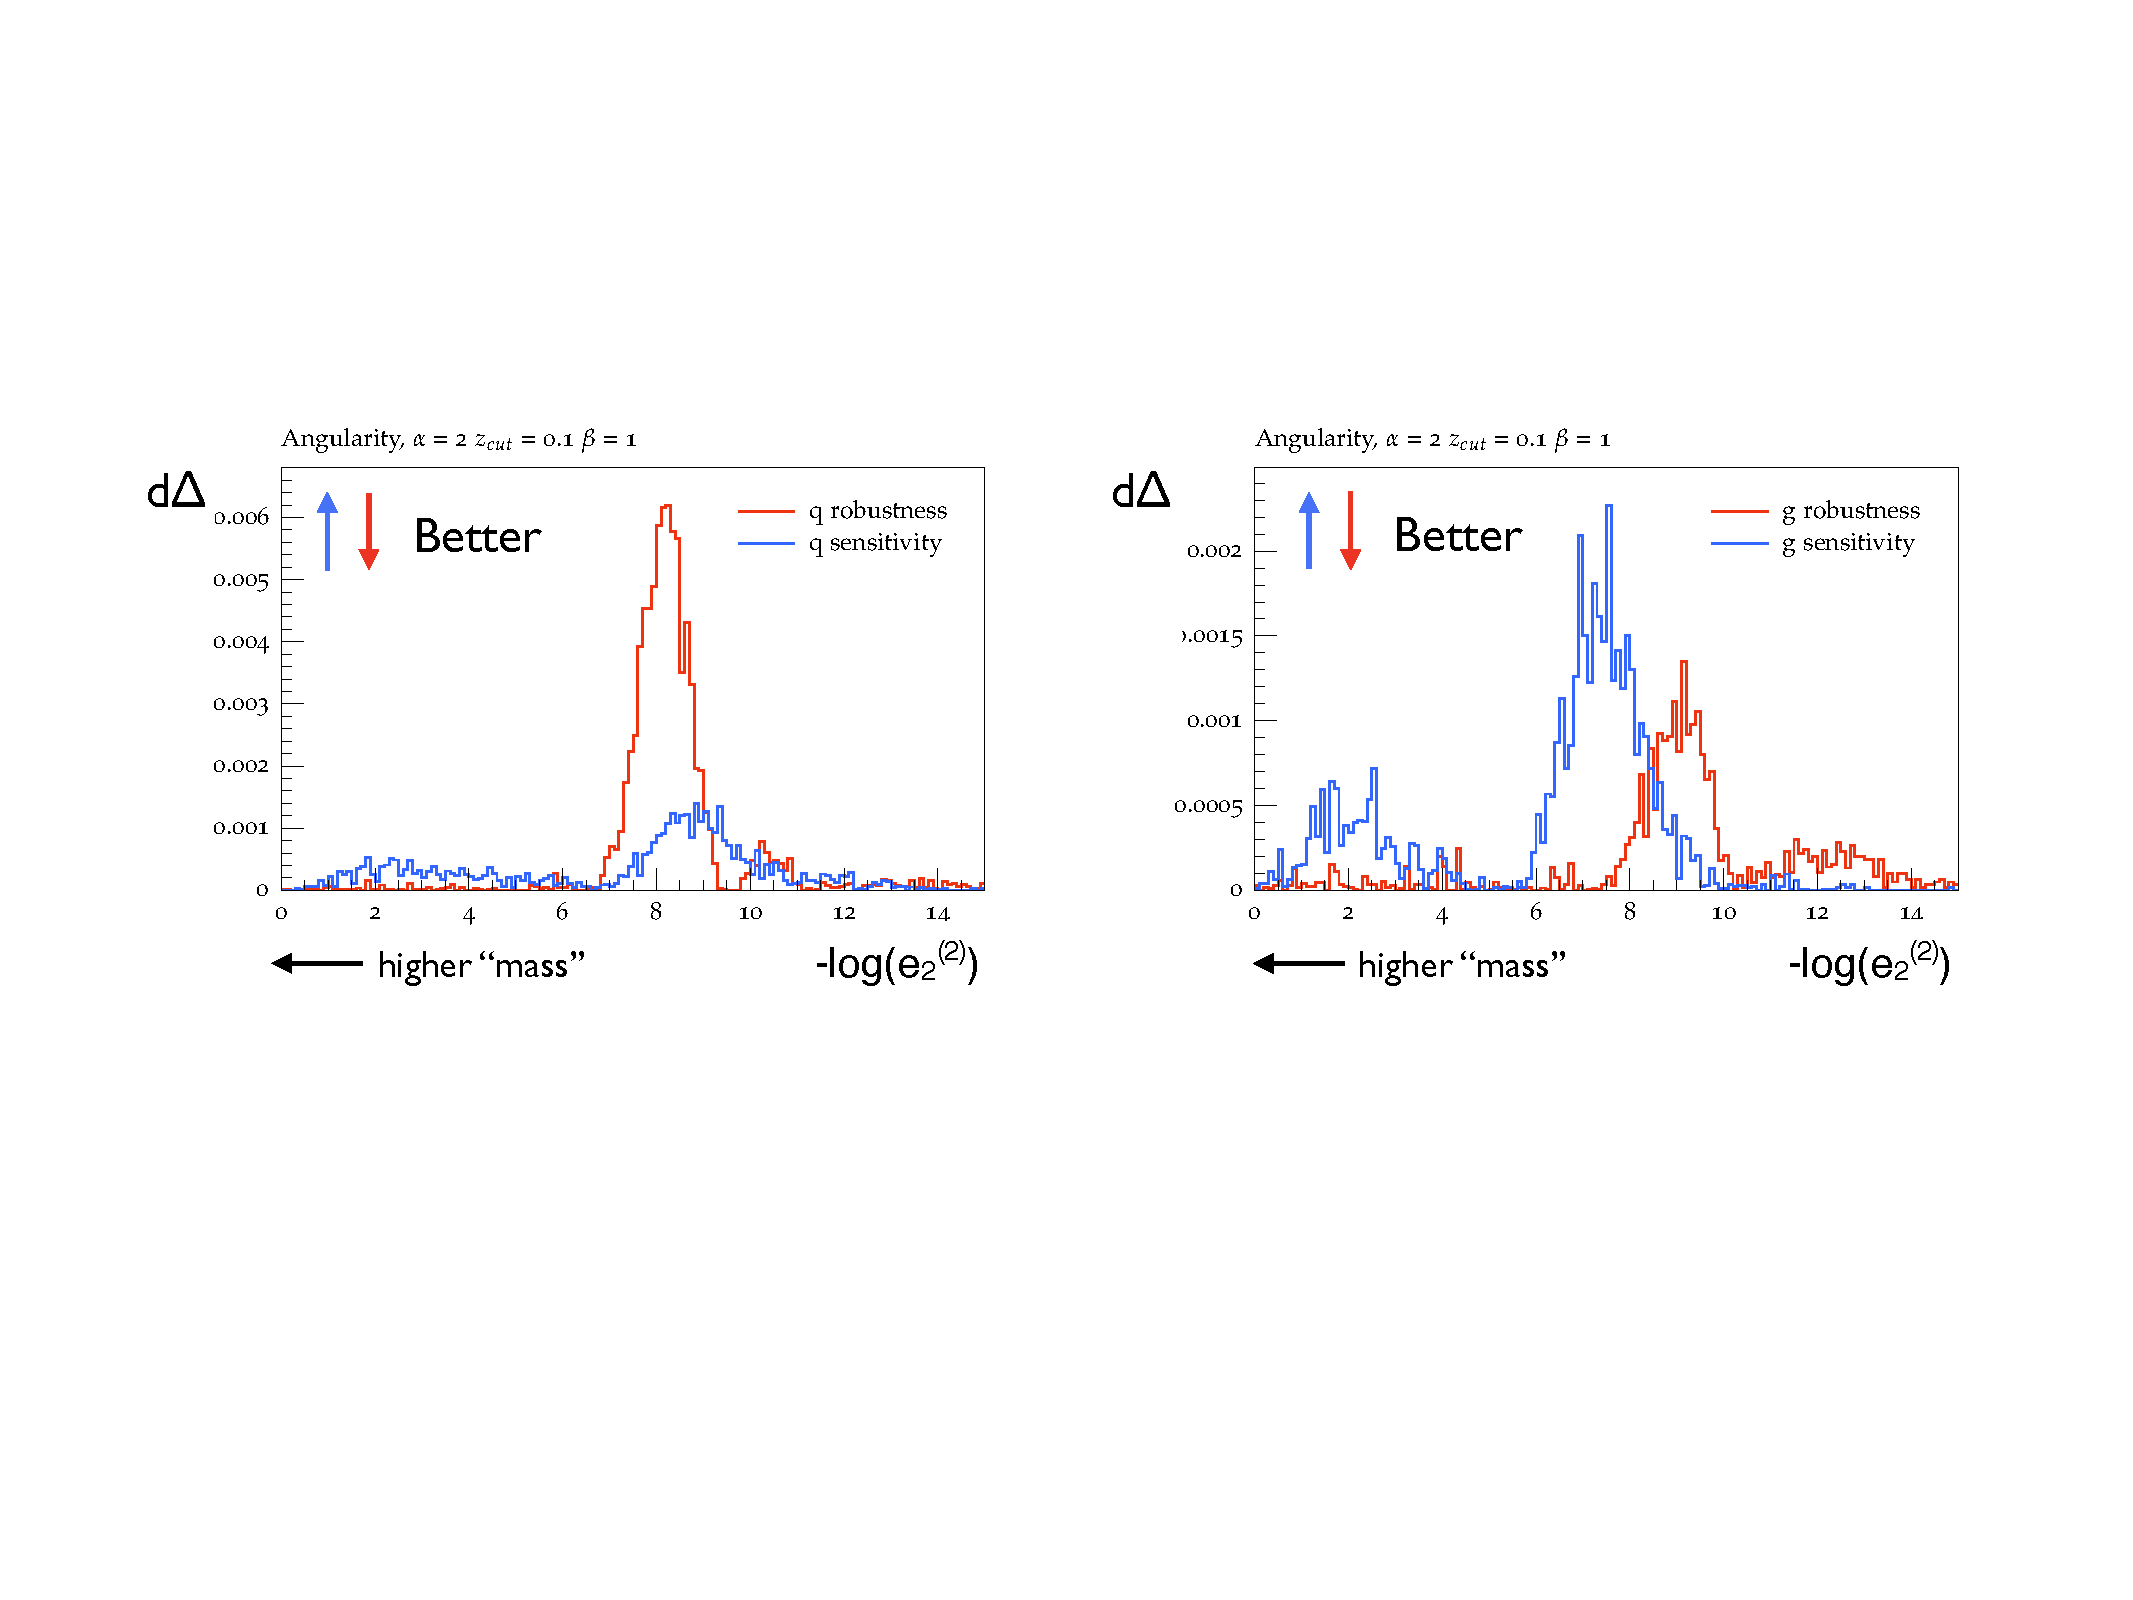
\includegraphics[width = 0.99\columnwidth]{jetsub_alphas_differentialseparation2.pdf}
\end{center}
\caption{The integrand of Eq.~\ref{jetsub_alphas_eq:seppower} in \textsc{Herwig~7}.  Shown is the normalized squared jet mass ($e_2^{(2)}$)  for quark jets (left) and gluon jets (right), with higher values of the mass are on the left.  The baseline $f$ function from Eq.~\ref{jetsub_alphas_eq:seppower} is the same for the red and blue curves.  For blue (sensitivity) the $g$ function is from varying $\alpha_s$ by 10\%, whereas for red (robustness) the $g$ function hadronization is turned off.  Note the different vertical scale in the left and right plots. }
\label{jetsub_alphas_fig:differentialseparation}
\end{figure}

The sensitivity to $\alpha_s$ is shown in Fig.~\ref{jetsub_alphas_fig:sensitivity}, in the case of normalized squared jet mass ($e_2^{(2)}$) for quark and gluon jets.
%
To the left of the low-mass NP peak, the shape of the $e_2^{(2)}$ distribution is nearly flat for quarks and nearly linear (in the log-space) for gluons, as expected from Eq.~\ref{jetsub_alphas_eq:ecf_ll_dsitribution}.
%
Increasing $\alpha_s$ shifts the quark distribution up but has nearly no impact on the shape of the distribution below the peak.
%
The size of the NP peak is significantly impacted by the value of $\alpha_s$, with smaller $\alpha_s$ values implying that NP effects are more important to the groomed mass distribution.
%
In contrast, the slope of the distribution for gluons does change with the variations in $\alpha_s$, but there is no low-mass NP peak.

The robustness to NP effects is shown in Fig.~\ref{jetsub_alphas_fig:robustness}, using the same $e_2^{(2)}$ distribution but now with variations in the modeling of hadronization and MPI effects.
%
Overall, there is excellent stability in the $e_2^{(2)}$ distribution.
%
The low-mass peak for quarks is almost entirely due to hadronization effects.
%
According to \textsc{Herwig~7}, the impact of hadronization is much smaller for gluon jets, as expected since perturbative effects push the distribution away from the NP-sensitive region in Eq.~\ref{jetsub_alphas_eq:np}.

Fig.~\ref{jetsub_alphas_fig:differentialseparation} shows the distribution of the differential separation power (integrand of Eq.~\ref{jetsub_alphas_eq:seppower}), using the variation with $\alpha_s$ as the sensitivity and the change from turning off hadronization as the robustness.
%
For quark jets, Figs.~\ref{jetsub_alphas_fig:sensitivity} and ~\ref{jetsub_alphas_fig:robustness} showed that the biggest variations with $\alpha_s$ occurred at low mass which is also where NP effects are largest.
%
This corresponds to the peak in the blue and red distributions in Fig.~\ref{jetsub_alphas_fig:differentialseparation} occurring in nearly the same location.
%
In contrast, the peaks are more well-separated in Fig.~\ref{jetsub_alphas_fig:differentialseparation} for gluon jets and the blue is shifted to higher mass values where there is more perturbative control.
%
This suggests that gluon-enriched samples are going to play an important role for $\alpha_s$ determination from jet substructure.

\begin{figure}[t]
\begin{center}
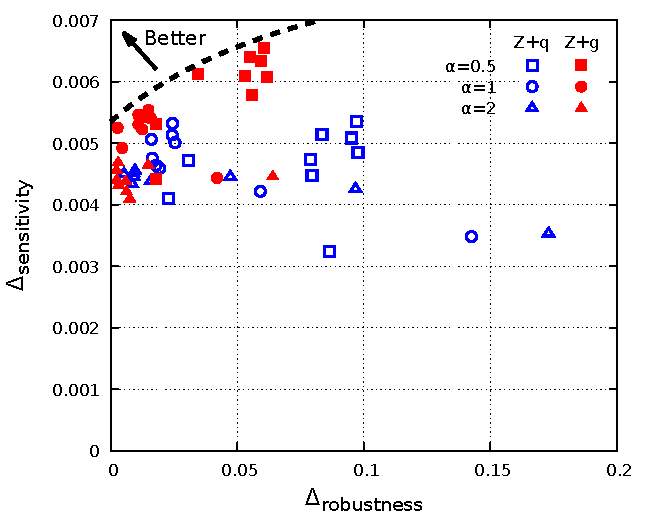
\includegraphics[width = 0.6\columnwidth]{jetsub_alphas_robsep.pdf}
\end{center}
\caption{The tradeoff between sensitivity and robustness for 27 two-point correlator/jet grooming combinations.  Open blue symbols represent quark jets and closed red symbols represent gluon jets.}
\label{jetsub_alphas_fig:robseptradeoff}
\end{figure}

A summary of the sensitivity-robustness tradeoff for many two-point correlators is presented in Fig.~\ref{jetsub_alphas_fig:robseptradeoff}.  As already observed for the jet mass, gluons tend to have superior sensitivity and robustness compared with quarks.
%
This is not surprising, as gluons have more perturbative radiation than quarks ($C_A>C_F$).
%
The jet mass has $(\Delta_\mathrm{sensitivity},\Delta_\mathrm{robustness})=(0.097,0.0043)$, $(0.015,0.0046)$ for quarks and gluons, respectively, using $\beta=0$ and $z_\mathrm{cut}=0.1$.
%
The groomed two-point correlators with the best quark and gluon sensitivity and robustness have $\alpha=1$, $z_\mathrm{cut}=0.05$ and $\beta=1$ or $\beta=2$.
%
The choice of $\alpha=1$ correspond to $k_t$ (a.k.a.~width) instead of mass, which may not be so surprising since the scale of $\alpha_s$ is set by $k_t$ and not mass.
%
Interestingly, $k_t$ with $\beta=0$ has significantly worse sensitivity than $\beta=1$ or $\beta=2$, highlighting the importance of having some double-logarithmic information. 
%
This study suggests that $k_t$ observables are important to include in future experimental and theoretical studies. The three-loop anomalous dimensions for the Energy-Energy Correlator (EEC) in $e^+e^-$, which is a $k_t$ sensitive observable, were recently derived \cite{Moult:2018jzp}. This will allow for a study of $k_t$ sensitive observables at N$^3$LL in $e^+e^-$, and a comparison with mass type observables. 
%
It would also be interesting to study how the robustness versus sensitivity picture changes when considering only subsets of the available observable range.

%%%%%%%%%%%%%%%%%%%%%%%%%%%
\subsection{The Issue of Casimir Scaling}
\label{jetsub_alphas_sec:casimir}
%%%%%%%%%%%%%%%%%%%%%%%%%%%

While we have illustrated that groomed jet mass provides excellent sensitivity to $\alpha_s$, particularly for gluon jets, one problem that is immediately clear from Sec.~\ref{jetsub_alphas_sec:analytic} is that the leading behavior of the distributions is always dominated by the product $\alpha_s C_i$.
%
While this is broken at higher perturbative orders, it implies that at lowest order there is a complete degeneracy of the value of $\alpha_s$ and the quark versus gluon fraction of jets.
%
This problem is not faced for dijet event shapes at $e^+e^-$ colliders, which are almost entirely quark dominated.

There are a variety of different approaches to overcome this problem, each with their own advantages and disadvantages.
%
First, the quark and gluon fractions are perturbatively calculable given the parton distribution functions (PDFs).
%
Therefore, perturbatively calculating the quark and gluon fractions inputs the most possible information, and should correspondingly lead to the best sensitivity for $\alpha_s$.
%
This has the downside, however, of also introducing sensitivity to the PDFs, which in principle should be fitted along with $\alpha_s$~\cite{Accardi:2016ndt}.
%
This difficulty also enters into other $\alpha_s$ extractions at the LHC, for example the $3$-$2$ jet rate~\cite{Chatrchyan:2013txa} or the energy-energy correlator~\cite{ATLAS:2015yaa,Aaboud:2017fml}.
%
One of the key hopes of using jet substructure was that the sensitivity to the PDFs could be minimized, but that is not the case if the quark and gluon fractions cannot be determined independently.

\begin{figure}[t]
\begin{center}
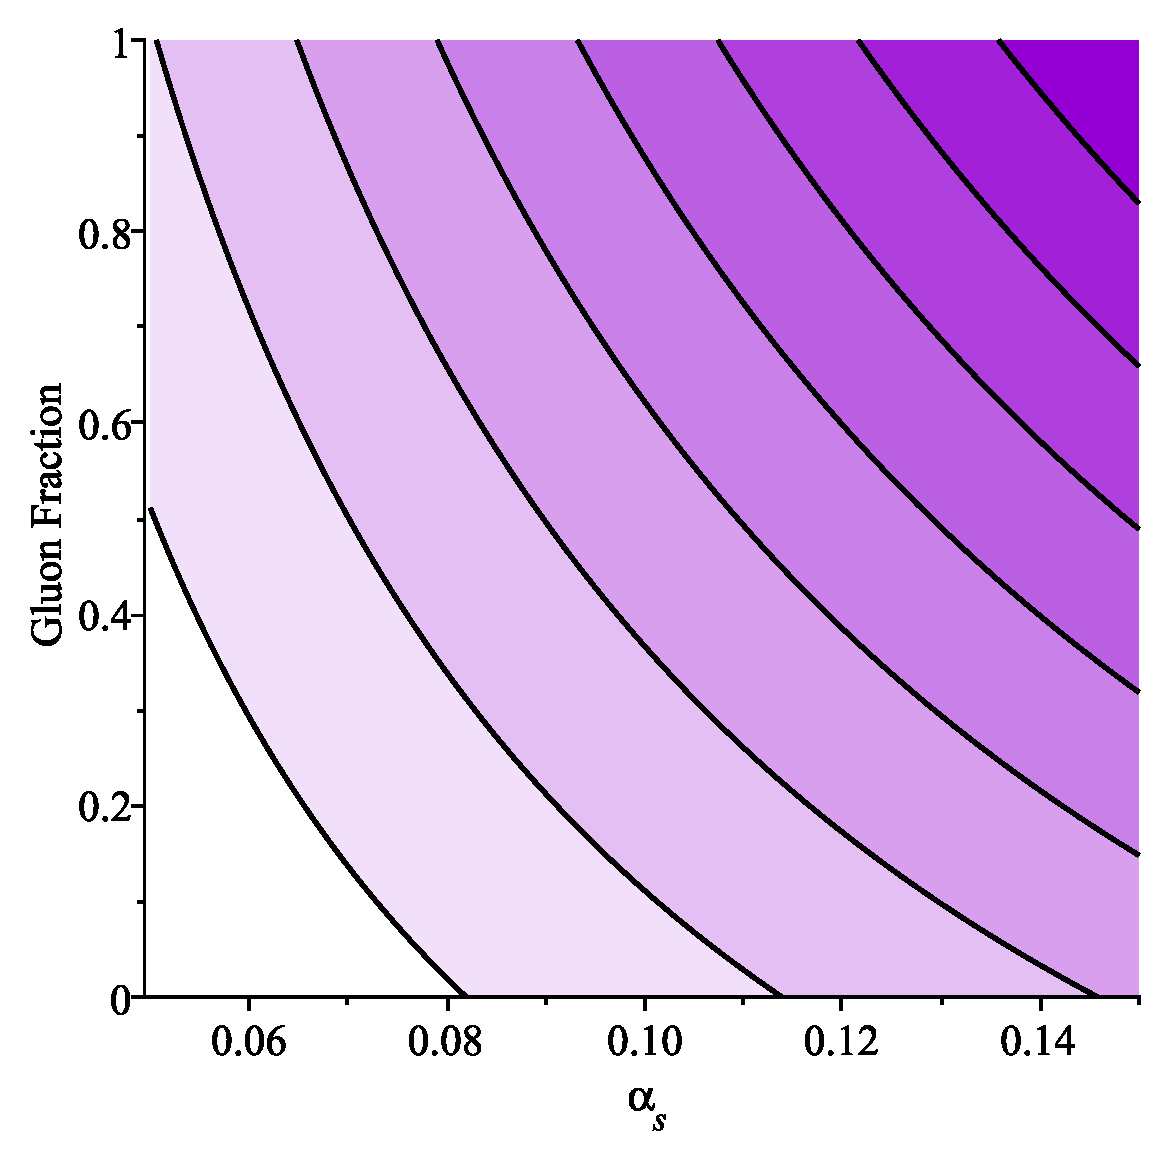
\includegraphics[width = 0.4\columnwidth]{jetsub_alphas_Degeneracy}
\end{center}
\caption{The slope of the probability distribution of $\log(e_2^{(2)})$ is proportional to $\alpha_s(C_Af_g+C_F(1-f_g))$, which is plotted above.  The degeneracy between $\alpha_s$ and $f_g$ (gluon fraction) are represented by the banana-shaped isocontours. }
\label{jetsub_alphas_fig:analyticbanana}
\end{figure}

A second approach is to simultaneously fit for $\alpha_s$ and the quark/gluon fraction.
%
In the resummation regime, the jet mass distribution only depends on $\alpha_s$ and the quark/gluon fraction.\footnote{At high mass, in the fixed-order regime, there is still residual explicit dependence on PDFs as is the case for the total cross-section.  This regime also suffers from sample-dependent effects where the quark and gluon substructure distributions have residual dependence on the hard process.}
%
Due to the fact that the two fractions must add to unity, this introduces a single additional parameter in the fit (see Fig.~\ref{jetsub_alphas_fig:analyticbanana}).
%
The degeneracy between the quark/gluon fraction and $\alpha_s$ is broken by higher order effects.
%
Furthermore, different $e_2^{(\alpha)}$ have different dependence on $\alpha_s$ and $C_i$ at higher orders.
%
Therefore, the measurement of multiple two-point correlators would allow the degeneracy to be broken.
%
From a theoretical perspective, this significantly complicates the analysis, since it would require precise
predictions to be made for the joint distribution of multiple two-point correlators.


In our fitting study in Sec.~\ref{jetsub_alphas_sec:ben_study}, we consider both of the above approaches.
%
It would be interesting to develop other approaches to disentangling the quark and gluon fractions and $\alpha_s$.
%
Without some kind of conceptual breakthrough, though, we expect that the quark/gluon fraction will be a limiting aspect of $\alpha_s$ extractions from jet substructure at the LHC.

%%%%%%%%%%%%%%%%%%%%%%%%%%%
\subsection{Normalized vs.\ Unnormalized Distributions}
\label{subjetsub_alphas_sec:norm}
%%%%%%%%%%%%%%%%%%%%%%%%%%%

In addition to the complication of quark and gluon fractions, another issue which appears for the extraction of $\alpha_s$ from jet substructure is the issue of normalization.\footnote{We thank Gavin Salam for interesting discussions on this topic. }
%
Unlike for $e^+e^-$ event shapes, the Born dijet cross section in $pp$ is sensitive to the value of $\alpha_s$.
%
This implies that the rate itself, in particular the absolute quark and gluon jet rates, carries information regarding $\alpha_s$. 

In our studies, we have decided to focus on using normalized distributions.
%
At a conceptual level, this is because we want to perform a true measurement of $\alpha_s$ from jet substructure, which is not dominated by the overall jet rate.
%
But there are two other practical concerns that favor using normalized distributions.

First, it is currently only possible to perform precise measurements of the groomed mass using normalized distributions.
%
Experimentally, the absolute rate is determined by the acceptance from kinematic requirements on the jet $p_\mathrm{T}$.
%
The sophisticated in-situ jet energy scale and resolution program carried out for small-radius jets~\cite{Aad:2014bia,Aaboud:2017jcu,Khachatryan:2016kdb,CMS-DP-2016-020} has not yet reached the same level of maturity for groomed large-radius jets.
%
That said, this is simply a matter of time, and experimental efforts have already started in this direction~\cite{ATLAS-CONF-2017-063}.
%
A key challenge that still remains is to fully understand the correlations in the calibrations and uncertainties between the jet energy and the jet substructure observables.

\begin{figure}[t]
\begin{center}
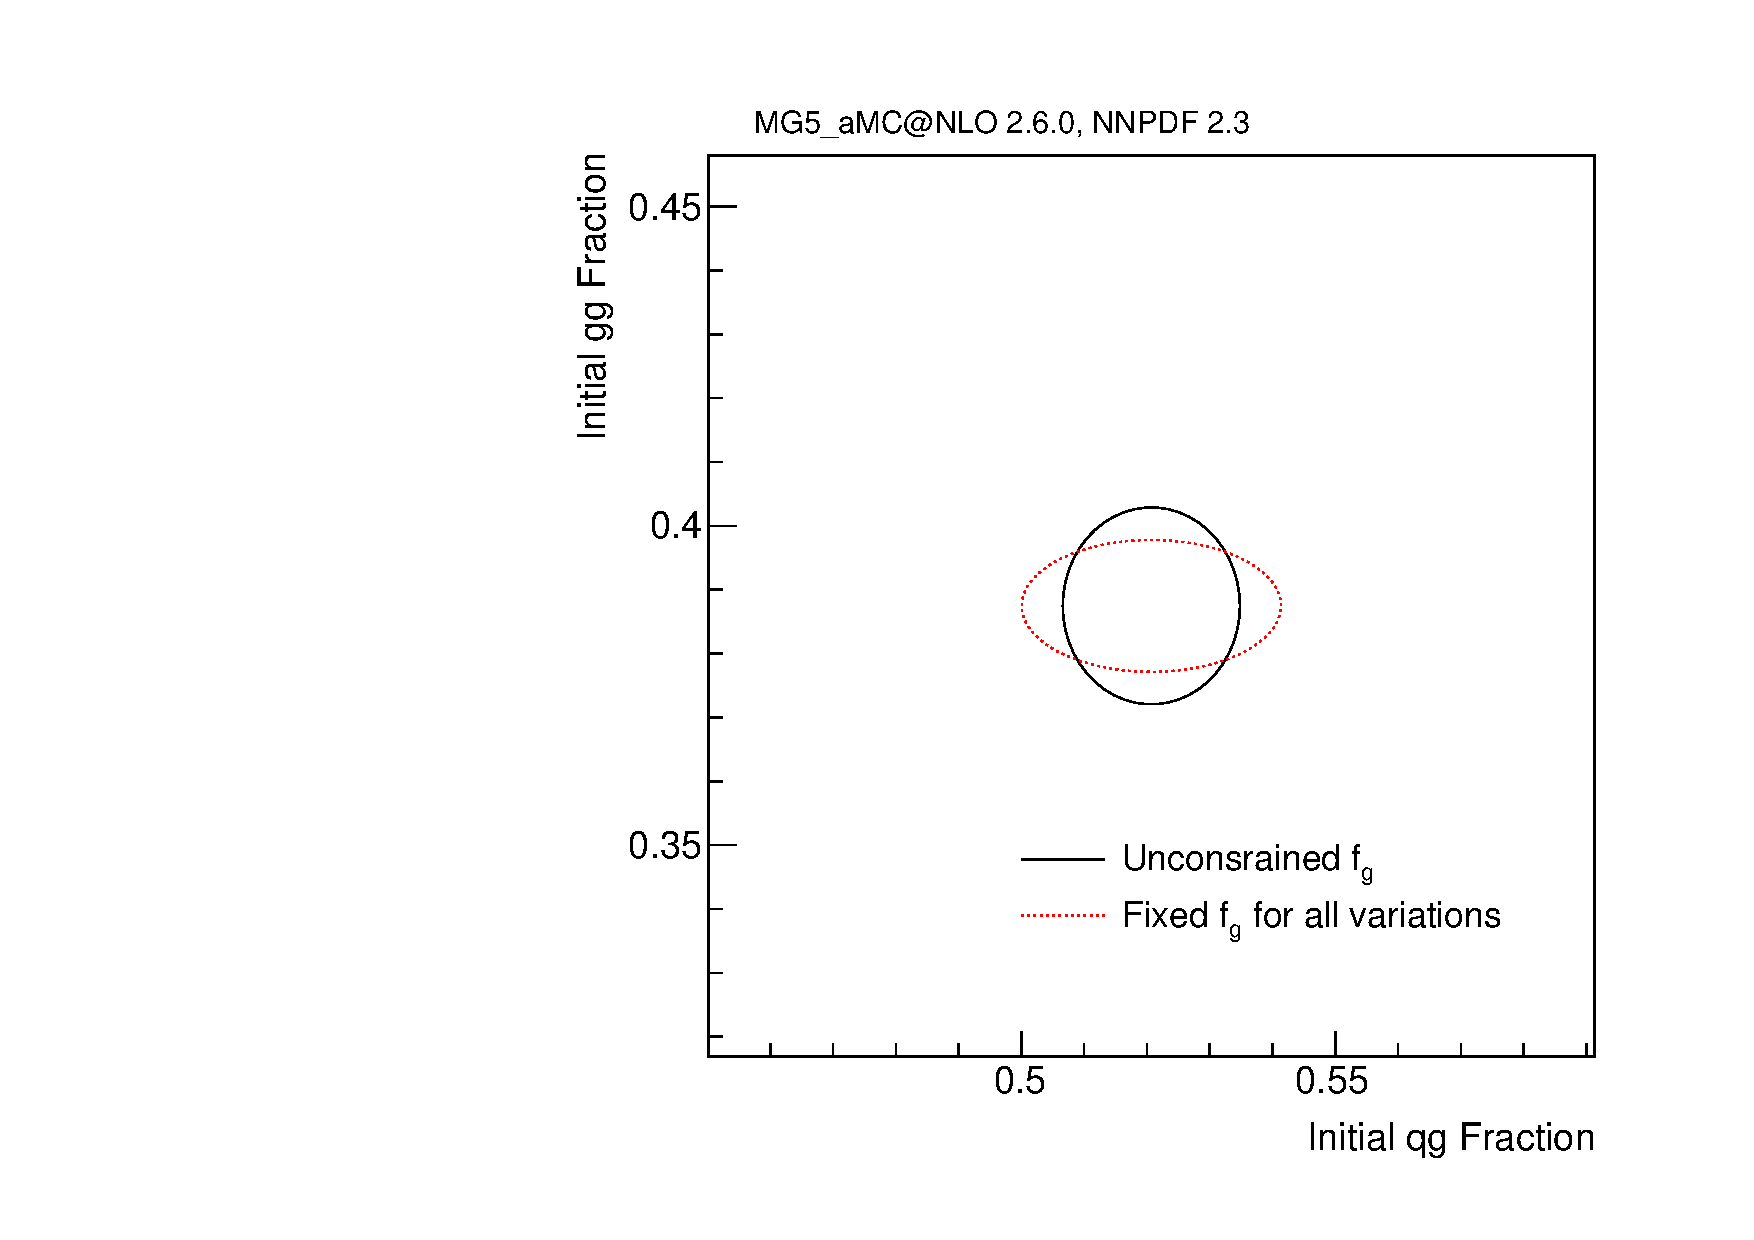
\includegraphics[width = 0.5\columnwidth]{jetsub_alphas_PDFs.pdf}
\end{center}
\caption{The fraction of $qg$ and $gg$ initial states for leading-order dijet production with $p_\mathrm{T}>200$ GeV, simulated at leading order with MG5\_aMC 2.6.0~\cite{Alwall:2014hca} using NNPDF 2.3~\cite{Ball:2012cx}.  The ellipses correspond to the uncertainty from the 100 error PDF sets.  For the red dashed line, the fraction of out-going gluon jets $f_g$ is constrained to be the same for all variations (and equal to the nominal PDF set).}
\label{jetsub_alphas_fig:pdf}
\end{figure}

Second, the use of normalized distributions minimizes the sensitivity to the PDFs.
%
As discussed in Sec.~\ref{jetsub_alphas_sec:pertsimplicity}, grooming renders the quark and gluon two-point-correlator distributions universal.
%
Therefore, the measured distribution only depends on the fraction of gluon jets $f_g$ that pass the event selection.
%
In contrast, the total cross-section depends on the relative proportions of all possible partonic initial states, which introduces a source of uncertainty that is not present for the normalized cross-section.
%
For example, the initial state could be one of $qq$, $qg$ or $gg$.
%
The relative proportions can be parameterized by two numbers $f_{qg}$ and $f_{gg}$ where $f_{qg}+f_{gg}=1-f_{qq}$.
%
Fig.~\ref{jetsub_alphas_fig:pdf} shows the uncertainty in $f_{qg}$ and $f_{gg}$ from leading-order PDFs.
%
Fixing $f_g$, which carries all of the PDF sensitivity for the shape measurement, has little effect on the uncertainty in $f_{qg}$ and $f_{gg}$.
%
Thus, using unnormalized distributions results in additional PDF sensitivity from also measuring the total cross-section in addition to the shape of the substructure distribution. 

From the perspective of perturbative accuracy, there is an important issue with using normalized distributions, which is that jet shape observables start at $\mathcal{O}(\alpha_s)$.
%
Specifically, the slope of the groomed mass distribution is $\mathcal{O}(\alpha_s)$.
%
This implies that to have an $\mathcal{O}(\alpha_s^2)$ uncertainty on the slope (as required to gain entry into the PDG world avarage), one needs to have $\mathcal{O}(\alpha_s^3)$ control, namely the NNLO $2 \to 3$ process for a jet with two constituents.
%
For the case of $e^+e^-$, this level of accuracy has been achieved, where the NNLO corrections to $e^+e^-\to 3$ jets are known and indeed used in the extractions of $\alpha_s$.
%
Due to recent progress in the calculation of the relevant amplitudes, we believe this is a realistic target for jet substructure, but clearly requires substantial further work.

\section{Idealized Performance at the LHC}
\label{jetsub_alphas_sec:ben_study}

The purpose of this section is to make some numerical estimates regarding $\alpha_s$ extraction from jet substructure at the LHC.
%
Many simplifying assumptions are made, with the goal of motivating a more complete effort within the context of ATLAS and CMS in collaboration with theorists.
%
First, we illustrate how $\alpha_s$ and the gluon fraction can be simultaneously extracted from the distribution of various two-point correlators.
%
Next, we estimate the needed experimental precision required to make a useful measurement of $\alpha_s$.
%
While both the theory and experimental precision will continue to improve over the next years, the community has already demonstrated that the work can begin with the first round of groomed jet mass results~\cite{Aaboud:2017qwh,CMS-PAS-SMP-16-010,Frye:2016aiz,Frye:2016okc,Marzani:2017mva,Marzani:2017kqd}.

\subsection{Extraction of Theory Templates}
\label{jetsub_alphas_sec:templates}

A complete extraction of $\alpha_s$ will require matching resummed results to high fixed order and also estimating NP effects.
%
The two sets of predictions for dijets thus far have been matched to LO~\cite{Frye:2016aiz,Frye:2016okc} and NLO~\cite{Marzani:2017mva,Marzani:2017kqd} and have used hadronization models to study NP corrections~\cite{Marzani:2017mva,Marzani:2017kqd}.
%
Performing high-order fixed-order matching is conceptually straightforward but computationally expensive; while this will be required eventually, we focus here on a demonstration without matching.
%
Therefore, we isolate the resummation regime,
\begin{equation}
\label{jetsub_alphas_eq:e2truncation}
\left. e_2^{(\alpha)}\right |_{\mathrm{NP}} \leq e_2^{(\alpha)}\leq z_\mathrm{cut}R^\alpha,
\end{equation}
%
where $\left. e_2^{(\alpha)}\right |_{\mathrm{NP}}$ is given in Eq.~\ref{jetsub_alphas_eq:np}, such that regions of phase space that are highly sensitive to NP or fixed-order effects are removed.
%
In this range, NLL calculations exist in analytic formulae that can be varied on-the-fly~\cite{Marzani:2017mva,Marzani:2017kqd}.
%
Figure~\ref{jetsub_alphas_fig:templates} shows the quark and gluon templates for $\alpha=\{1,2\}$ and $\beta=\{0,1\}$, truncated according to Eq.~\ref{jetsub_alphas_eq:e2truncation}.


\begin{figure}[t]
\begin{center}
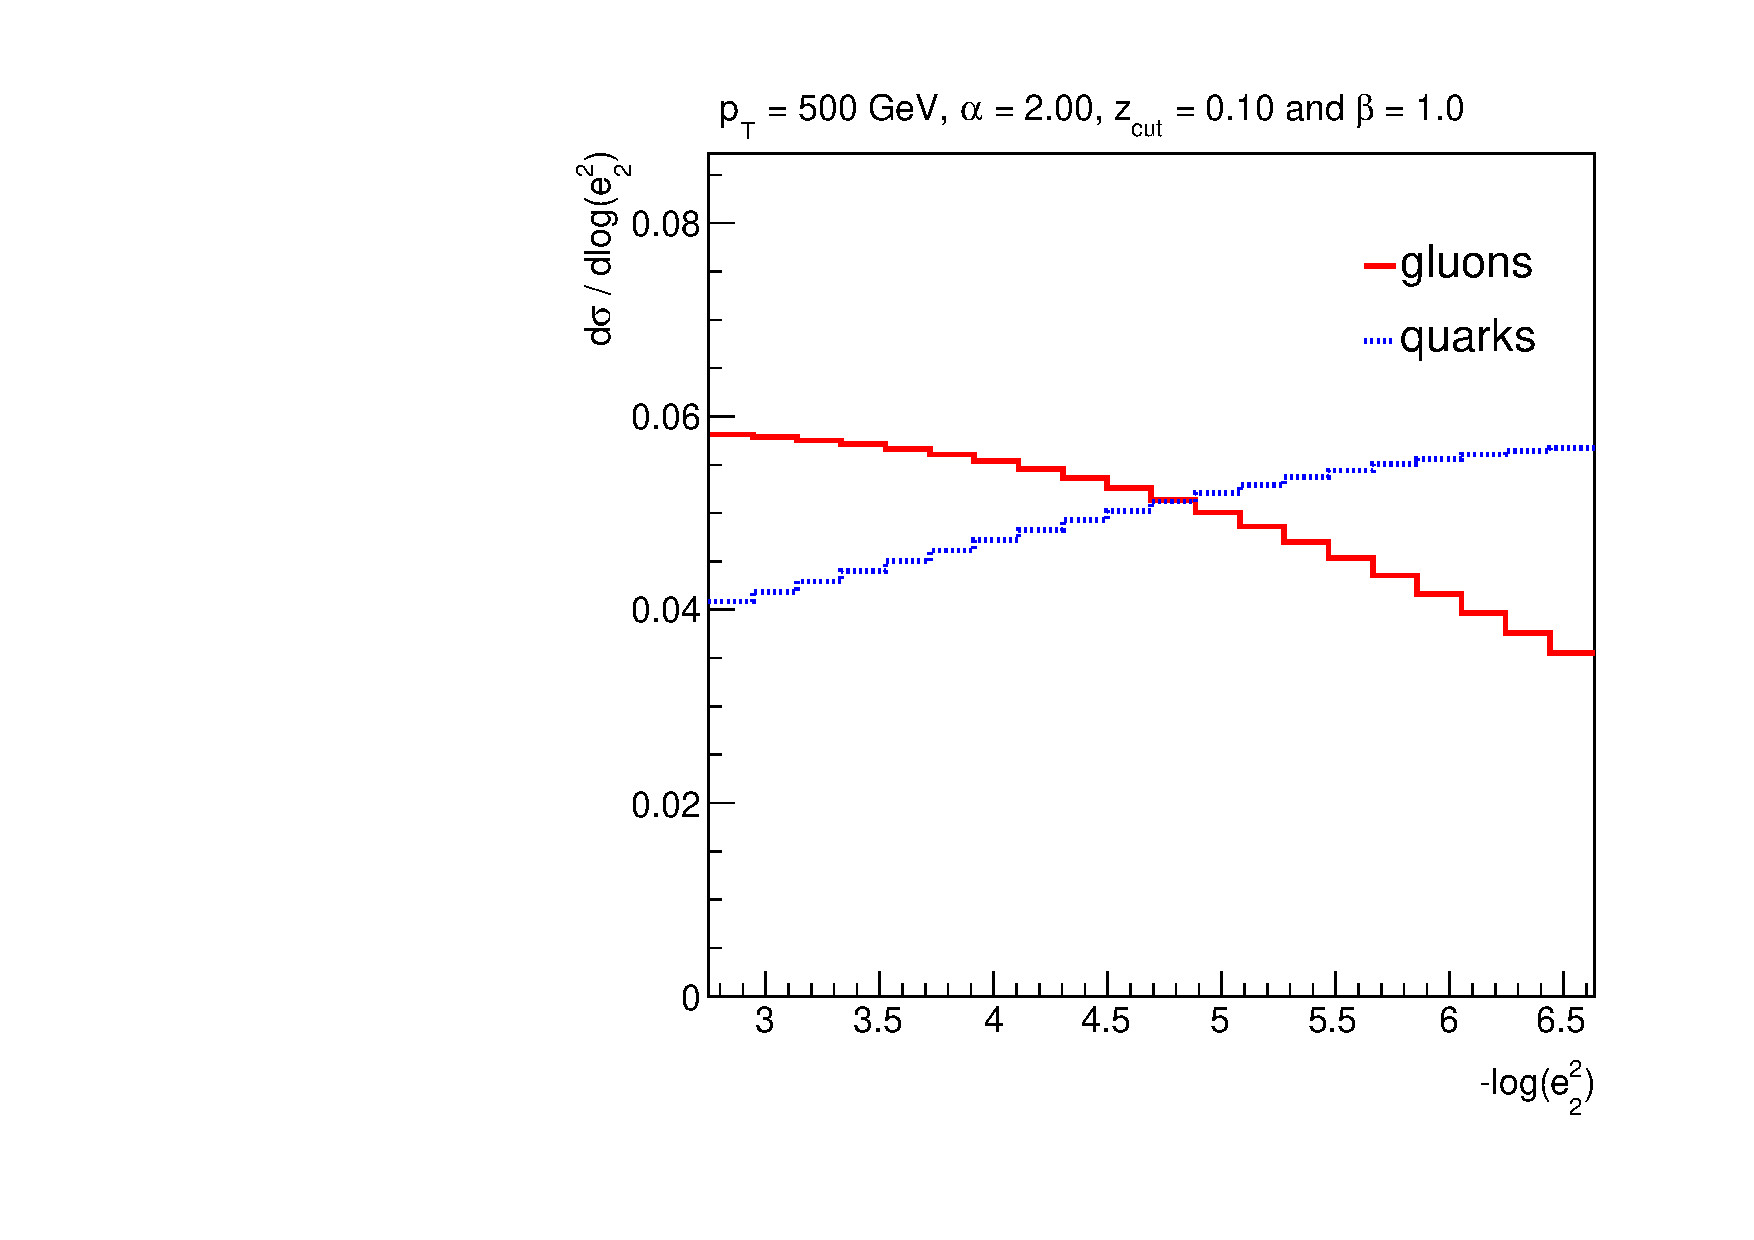
\includegraphics[width = 0.49\columnwidth]{jetsub_alphas_PDFs_alpha_20zcut1_beta_1023451324.pdf}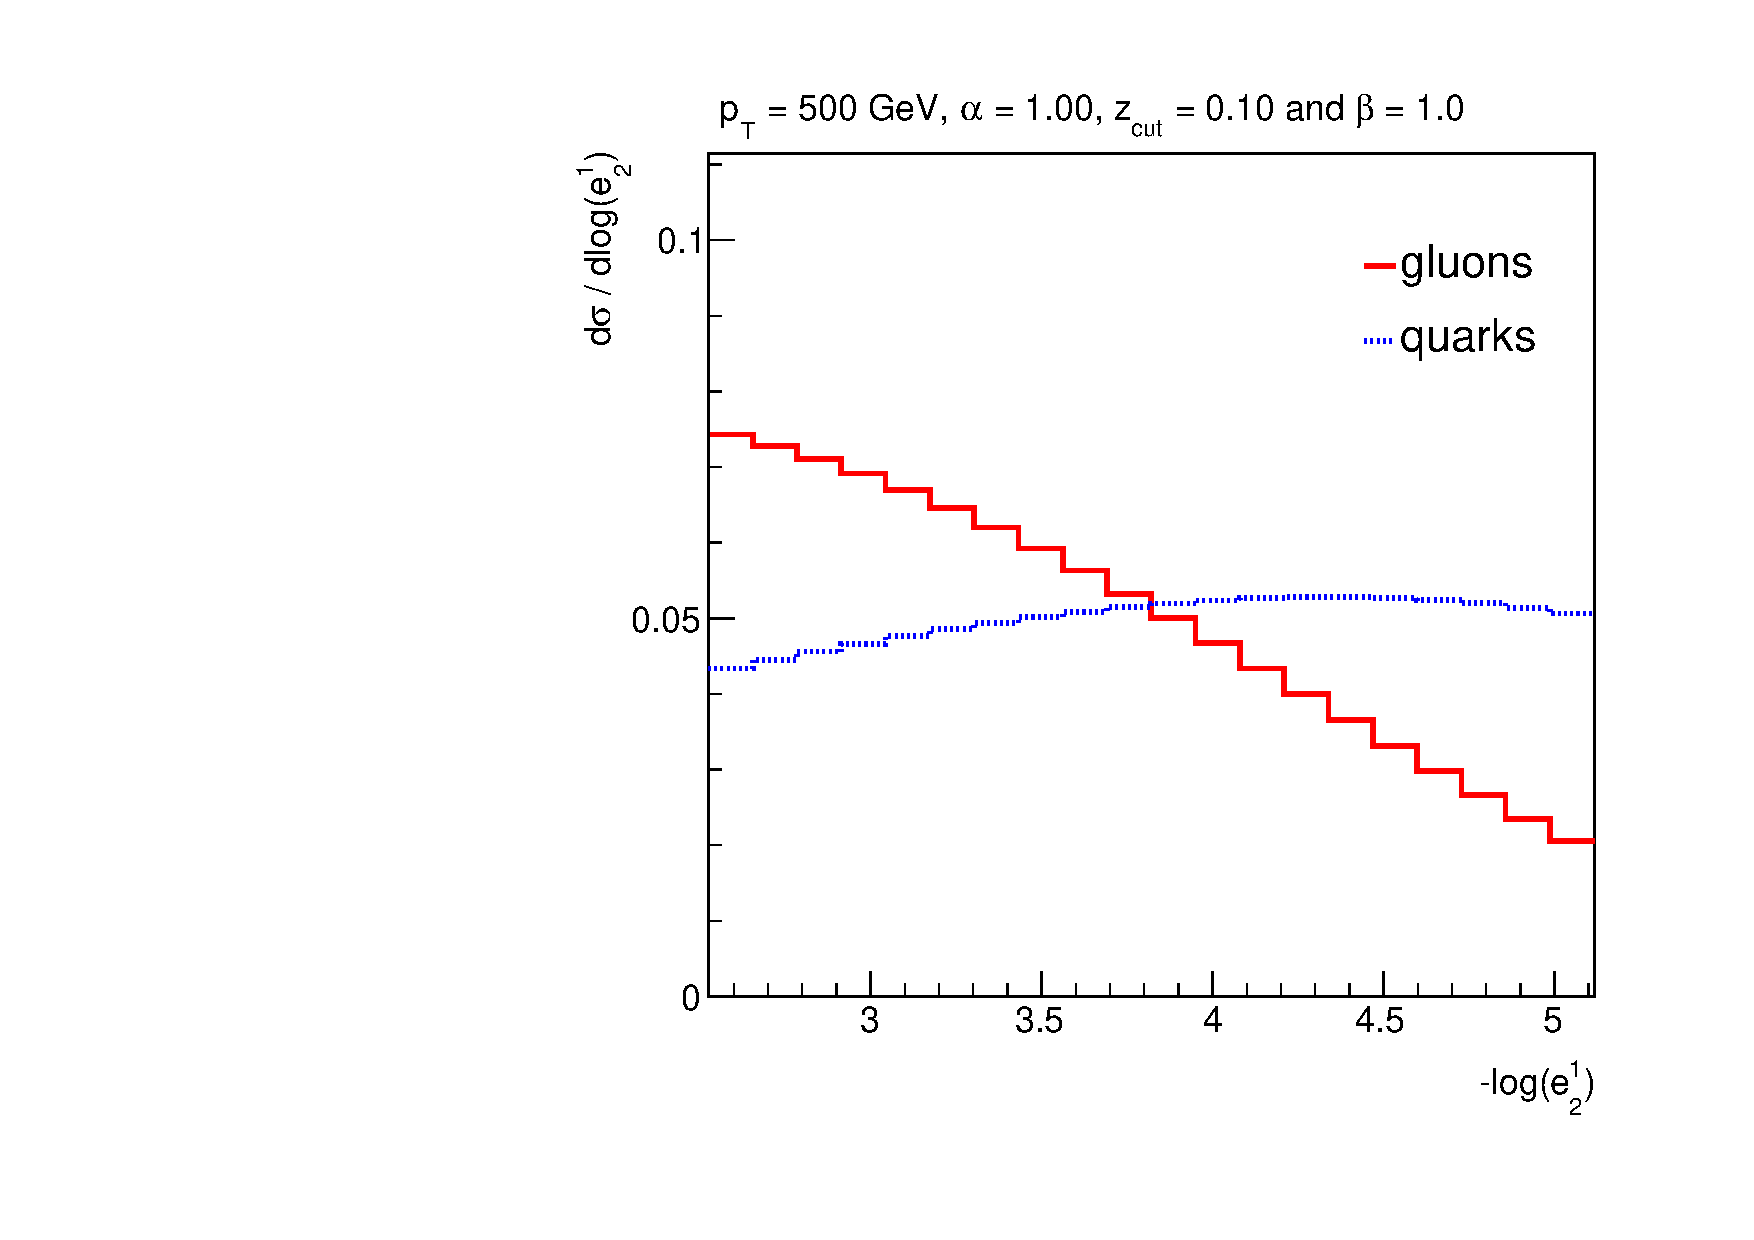
\includegraphics[width = 0.49\columnwidth]{jetsub_alphas_PDFs_alpha_10zcut1_beta_1023451324.pdf}\\
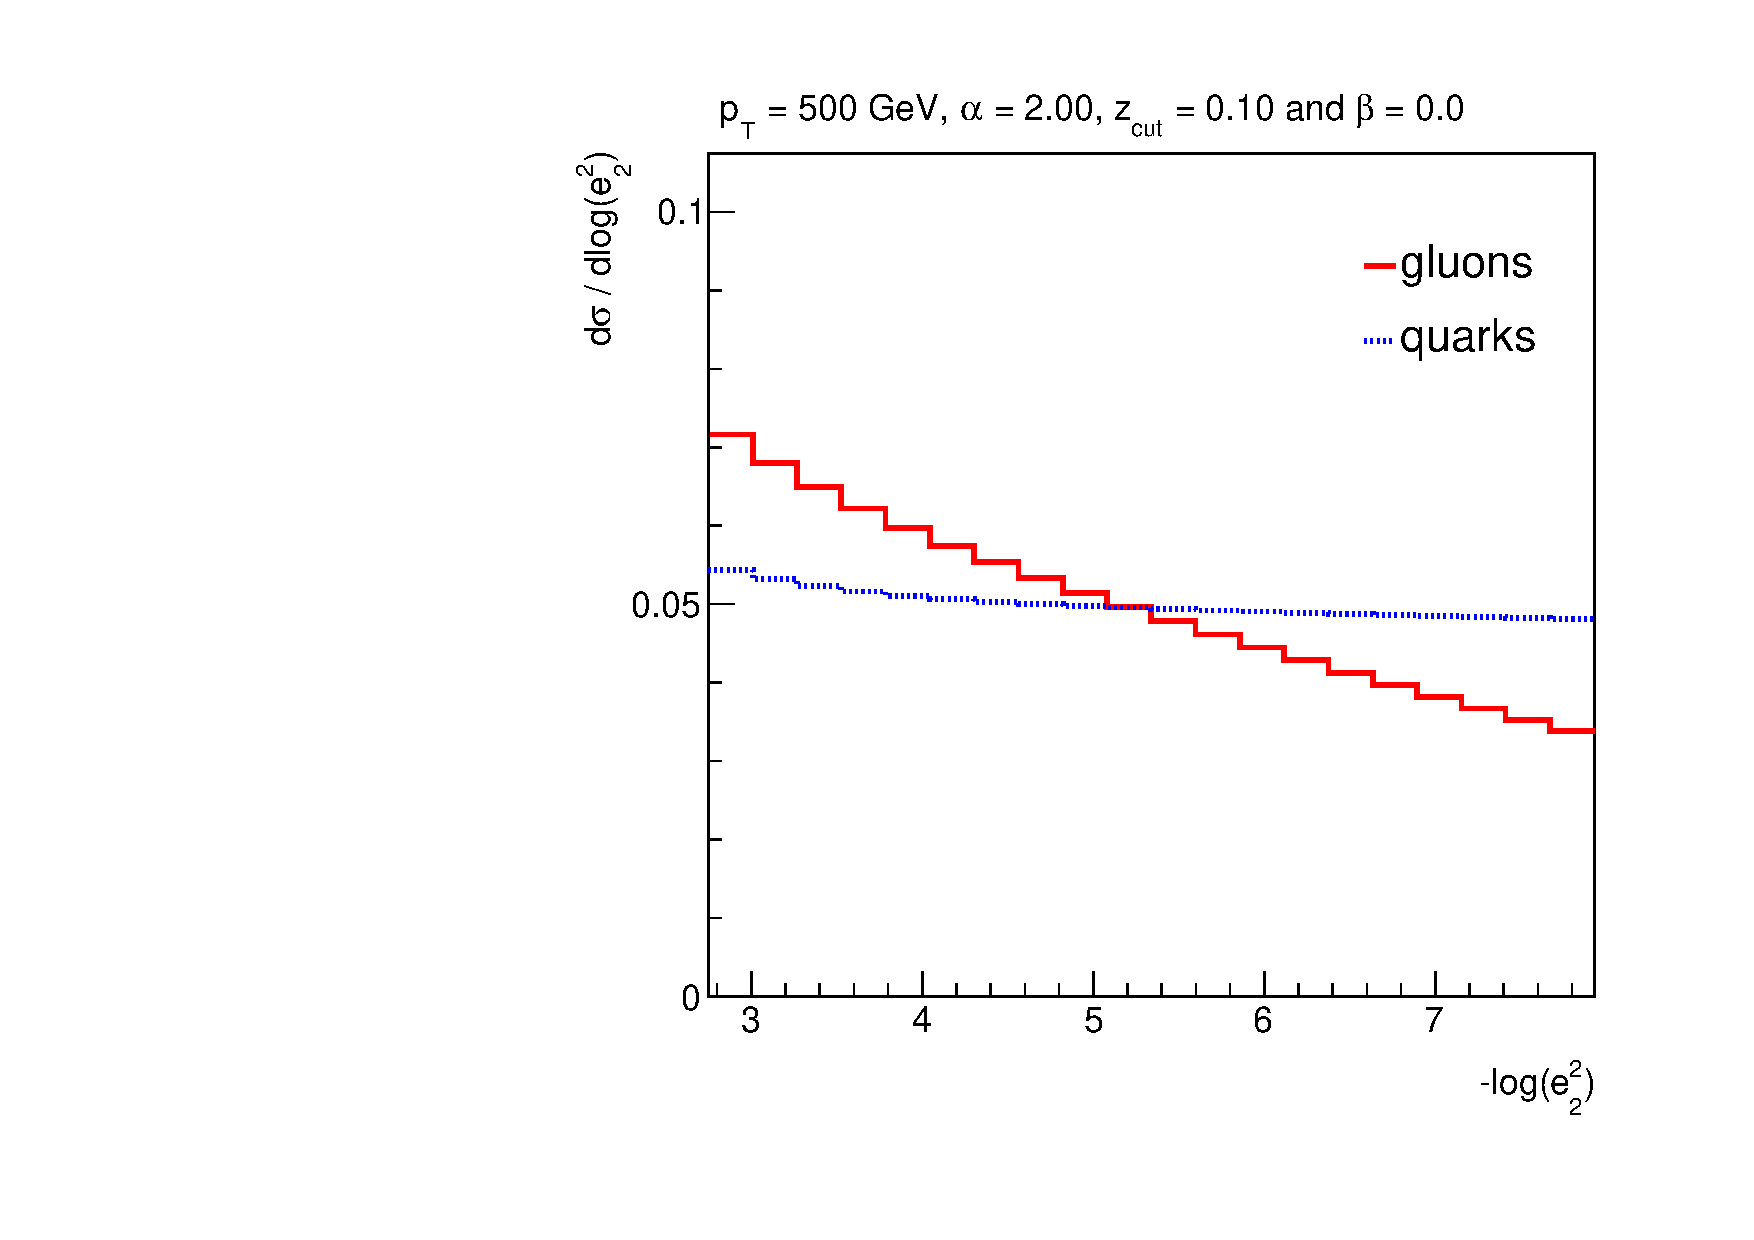
\includegraphics[width = 0.49\columnwidth]{jetsub_alphas_PDFs_alpha_20zcut1_beta_023451324.pdf}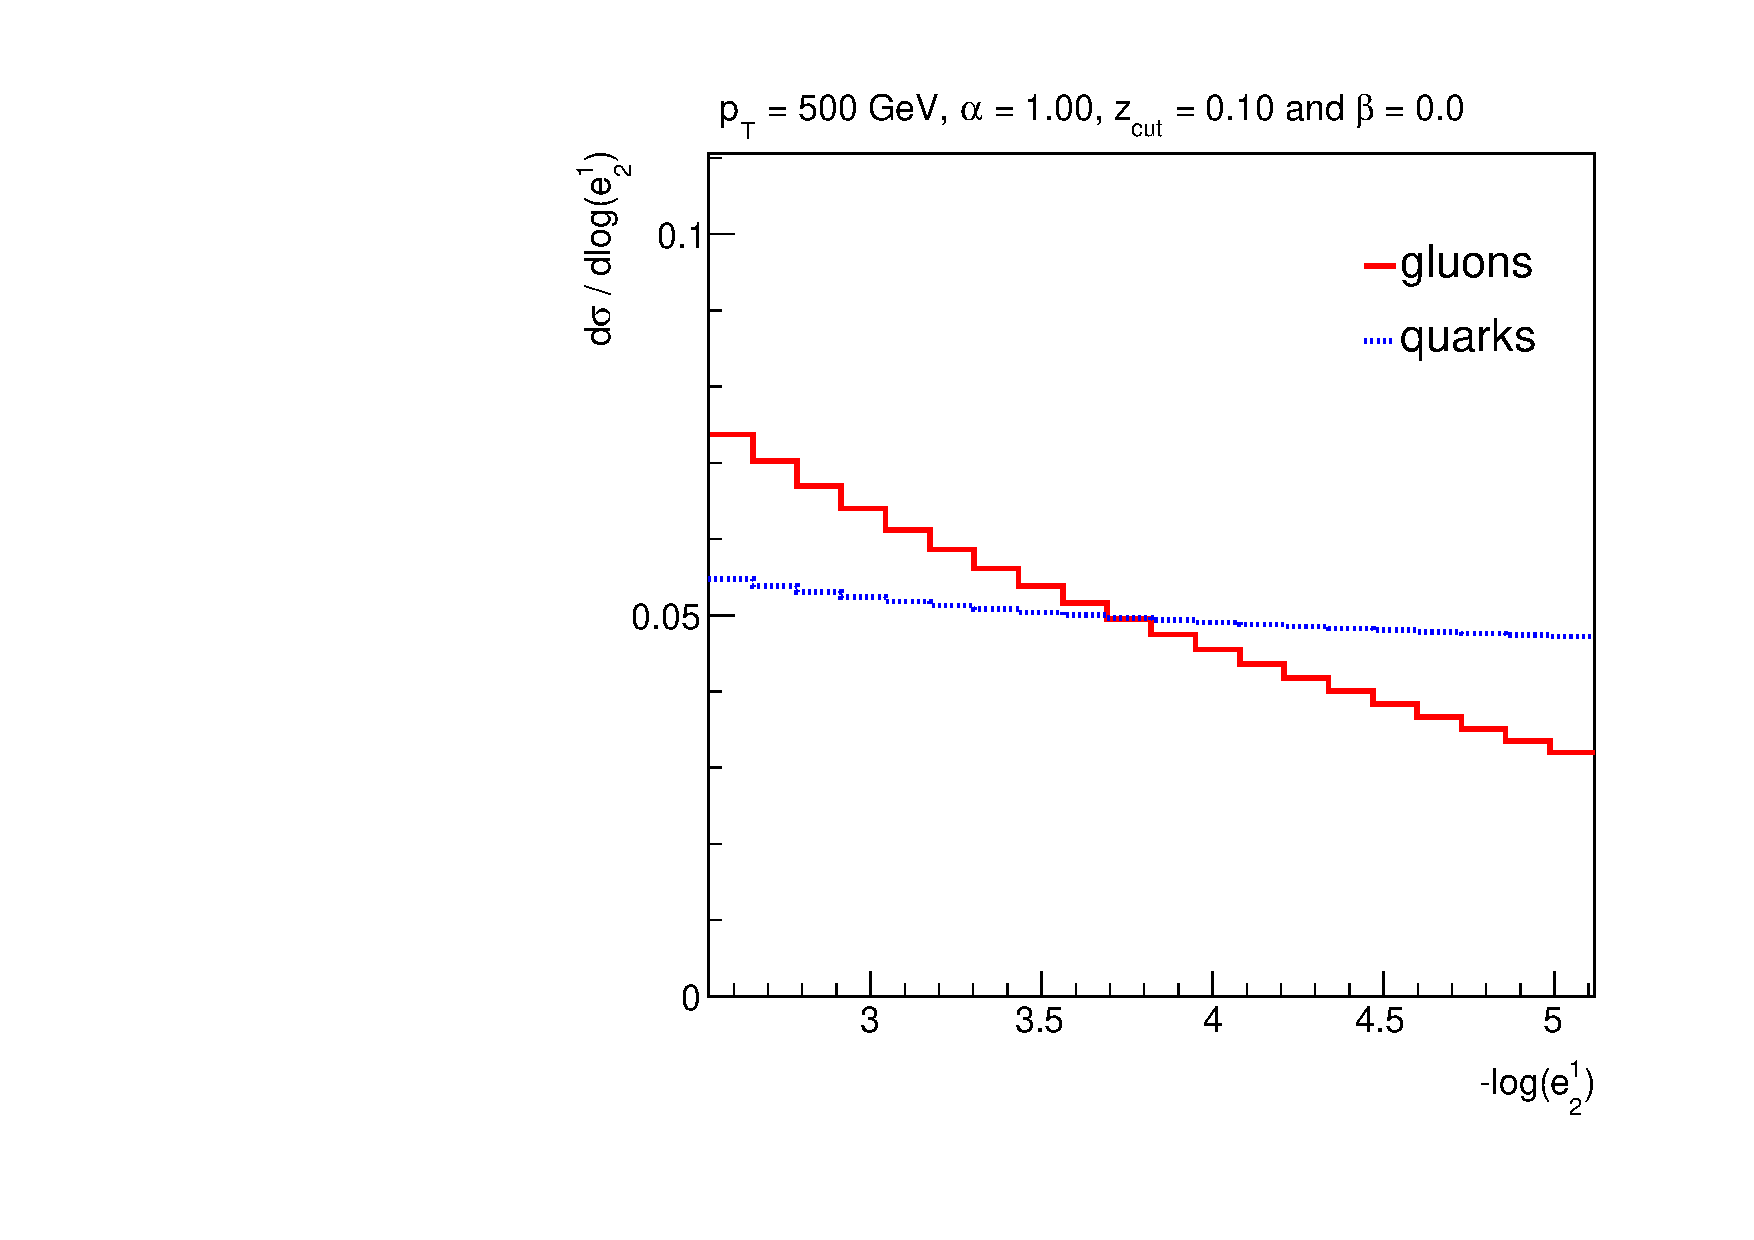
\includegraphics[width = 0.49\columnwidth]{jetsub_alphas_PDFs_alpha_10zcut1_beta_023451324.pdf}
\end{center}

\caption{The quark and gluon templates, computed at NLL~\cite{Marzani:2017mva,Marzani:2017kqd} for $\alpha=2$ (left column) and 
  $\alpha=1$ (right column), with grooming parameters $z_{\mathrm{cut}}  = 0.1$ and $\beta = 1$ (top row) and $\beta = 0$ (bottom row).  Note that larger masses are on the left so that the NP regime is on the
  right and the fixed-order regime is on the left.}
\label{jetsub_alphas_fig:templates}
\end{figure}

From these NLL distributions, pseudo-data are then generated from the binned analytic probability distribution $t(\alpha_s,f_g)$.
%
These distributions are a superposition of the quark and gluon distributions and depend only on $\alpha_s$ and $f_g$.
%
Each pseudo-dataset has $n$ events and its binned representation is denoted by $h(\alpha_s,f_g,n)$.
%
For a given pseudo-dataset, the fitted values of $\alpha_s$ and $f_g$ are determined from a $\chi^2$-like fit:
%
\begin{equation}
\label{jetsub_alphas_eq:chi2fit}
\alpha_s,f_g=\mathrm{argmin} \sum_i \frac{\left(h_i(\alpha_s,f_g,n)-t_i(\alpha_s,f_g)\right)^2}{\sigma(h_i(\alpha_s,f_g,n))^2},
\end{equation}
%
where $t_i, h_i$ are the bin content of histograms $t$ and $h$, and $\sigma(h_i)$ is the statistical uncertainty in bin $i$ of histogram $h$.
%
In practice, there would also be systematic uncertainties (see Sec.~\ref{jetsub_alphas_sec:resolution}), but the purpose of this study is to simply illustrate the sensitivity to $\alpha_s$ and $f_g$ for a given number of events.


	
\begin{figure}[t]
\begin{center}
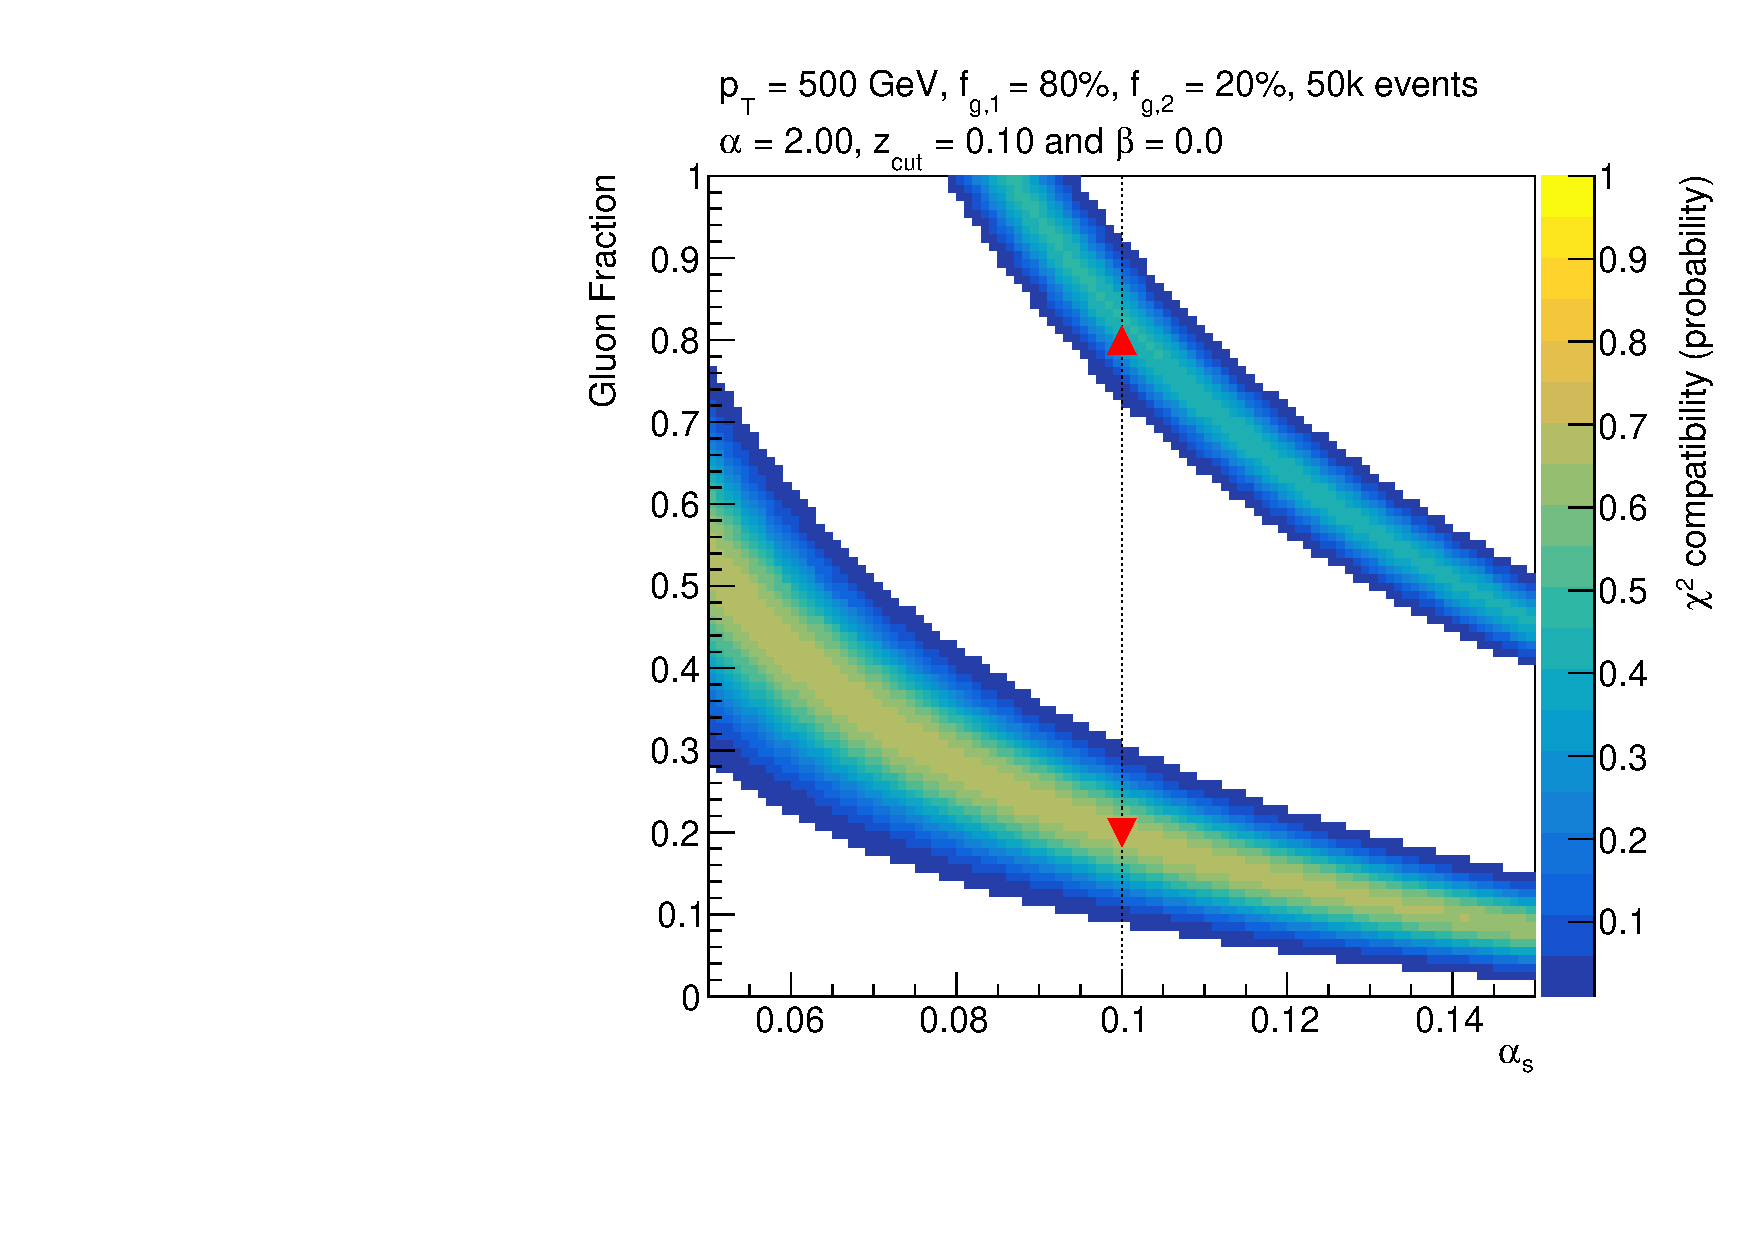
\includegraphics[width = 0.49\columnwidth]{jetsub_alphas_banana_alpha_20beta_0_zcut_123451324.pdf}
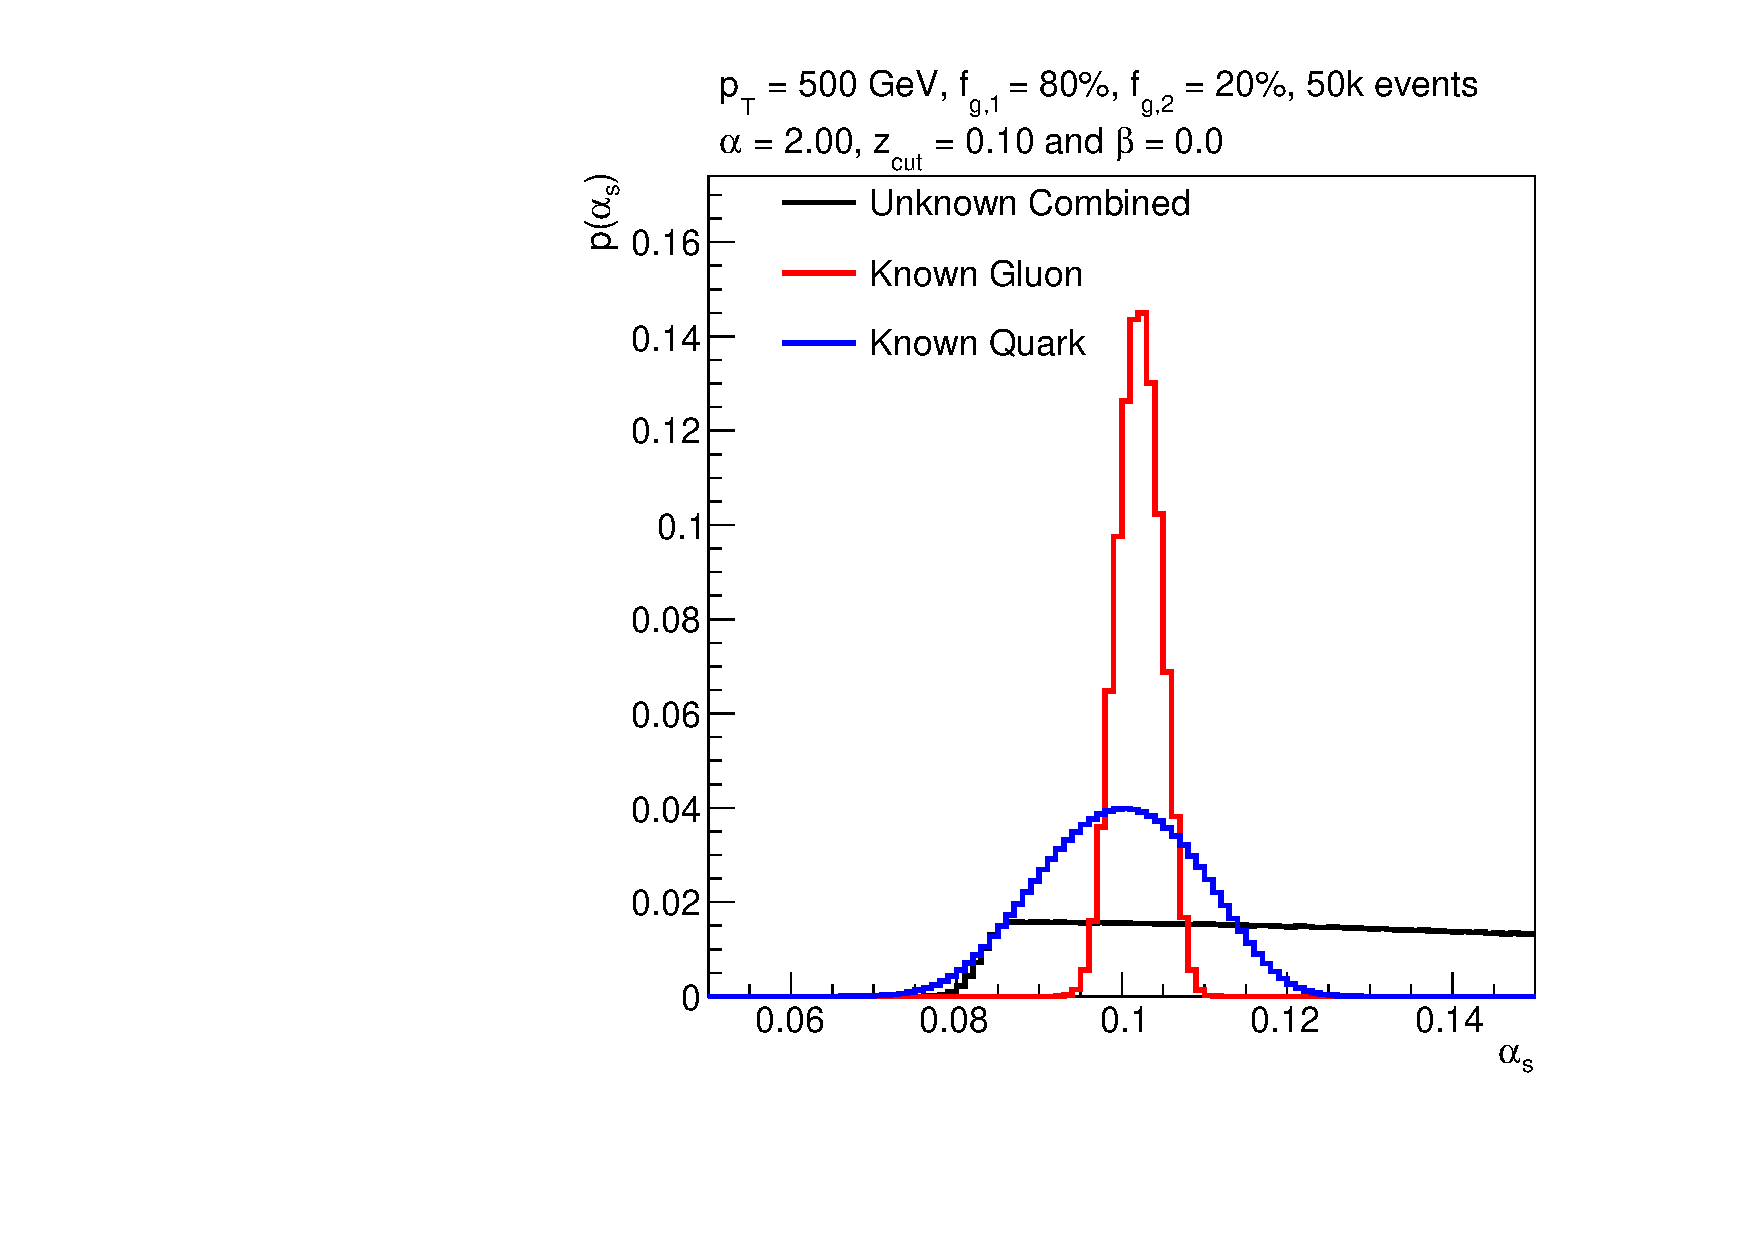
\includegraphics[width = 0.49\columnwidth]{jetsub_alphas_palpha_alpha_20beta_0_zcut_123451324.pdf}
\end{center}
\caption{Left: the probability of the minimized $\chi^2$ (assuming $n_\mathrm{bins}-1$ degrees of freedom) from Eq.~\ref{jetsub_alphas_eq:chi2fit} as a
  function of $f_g$ and $\alpha_s$ for one sample with 80\% gluons and another sample with 80\% quarks.  The true value of $\alpha_s$ is 0.1, as indicated by triangle markers.  Right: The right plot marginalized over $f_g$ and normalized to unity.  The three lines correspond to the fit performed on a pure sample of quarks, a pure sample of gluons, or a mixed sample of ($f_g\in\{0.2,0.8\}$) where the fractions are not known a priori.  This is the result from one pseudo-experiment with 100k events.}
\label{jetsub_alphas_fig:alpha2fit}
\end{figure}



%
An example fit is demonstrated in Fig.~\ref{jetsub_alphas_fig:alpha2fit} for the case of $\alpha=2$ and $\beta = 0$.
%
The left plot of Fig.~\ref{jetsub_alphas_fig:alpha2fit} shows the $\chi^2$ from Eq.~\ref{jetsub_alphas_eq:chi2fit} for two samples, one with 20\% gluons and one with 80\% gluons.
%
The true value is taken to be $\alpha_s=0.1$, and as expected, the $\chi^2$ probability is high for $f_g=0.2$ and $f_g=0.8$.%
\footnote{It is not necessarily peaked at this value because this is the result of one pseudo-experiment.  Averaging over many pseudo-experiments results in peaks at $f_g=0.2$ and $0.8$.}
%
The banana shapes of the curves are a consequence of the degeneracy due to Casimir scaling discussed in Sec.~\ref{jetsub_alphas_sec:casimir}.
%
From one sample alone, there is essentially no ability to distinguish between a larger $\alpha_s$ and a smaller $f_g$; the only constraint comes from the fact $0\leq f_g\leq 1$ which results in a crude bound on $\alpha_s$.
%
This is shown in the right plot of Fig.~\ref{jetsub_alphas_fig:alpha2fit} where the distribution is marginalized over $f_g$ and normalized to unity.
%
One can view this as the posterior probability of the fitted $\alpha_s$: the peak is the fitted value of $\alpha_s$ and the width is the uncertainty.
%
When $f_g$ is known, the uncertainty in $\alpha_s$ is significantly reduced; this is illustrated with pure quark and gluon samples.
%
Due to the larger color factor, the measurement with pure gluon jets is more sensitive to $\alpha_s$ than the fit using pure quark jets, as anticipated in Sec.~\ref{jetsub_alphas_sec:analytic}.
%
Using both the $f_g=0.2$ and $f_g=0.8$ samples to fit for $\alpha_s$, one can extract a $\sim 30\%$ measurement of $\alpha_s$, but there is no clear peak at the correct value of $\alpha_s$ due to the Casimir degeneracy.  

\begin{figure}[t]
\begin{center}
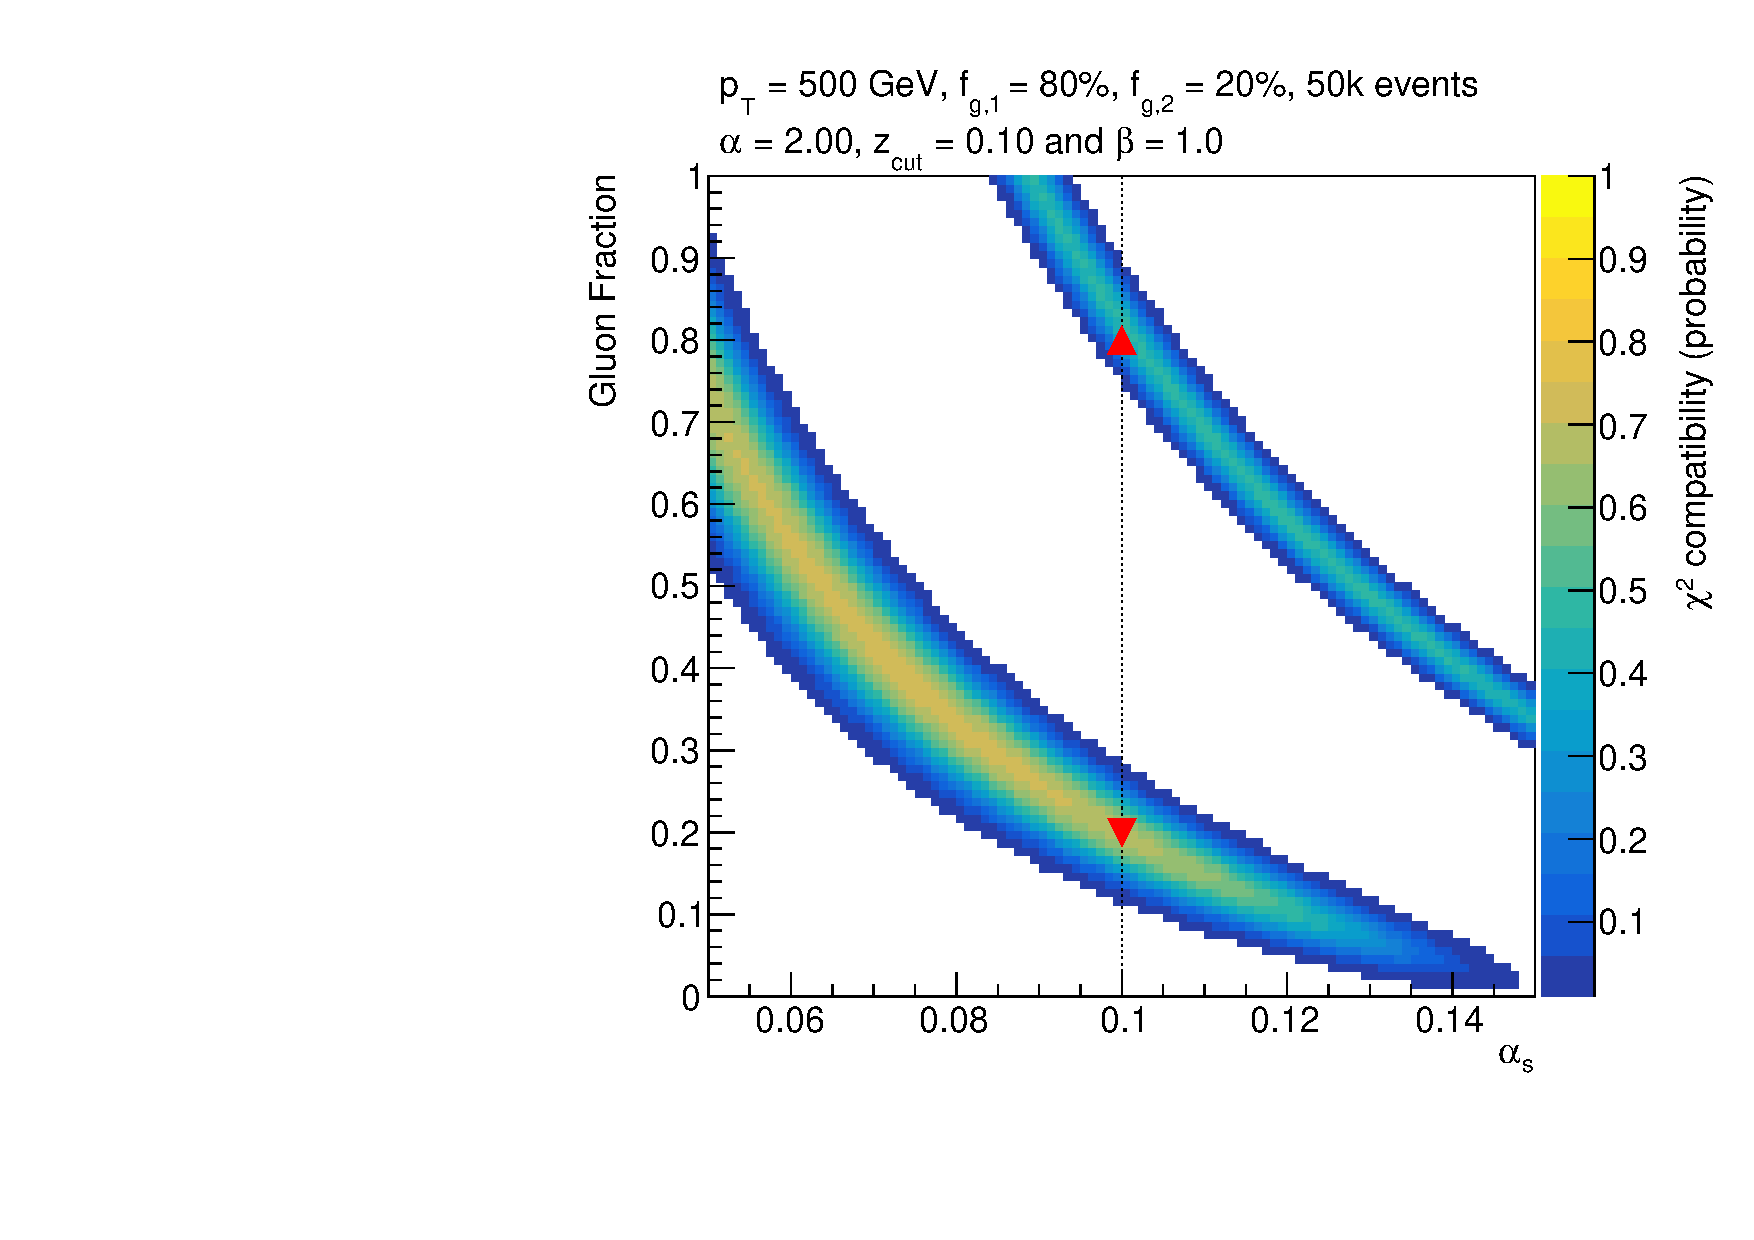
\includegraphics[width = 0.32\columnwidth]{jetsub_alphas_banana_alpha_20beta_10_zcut_123451324.pdf}
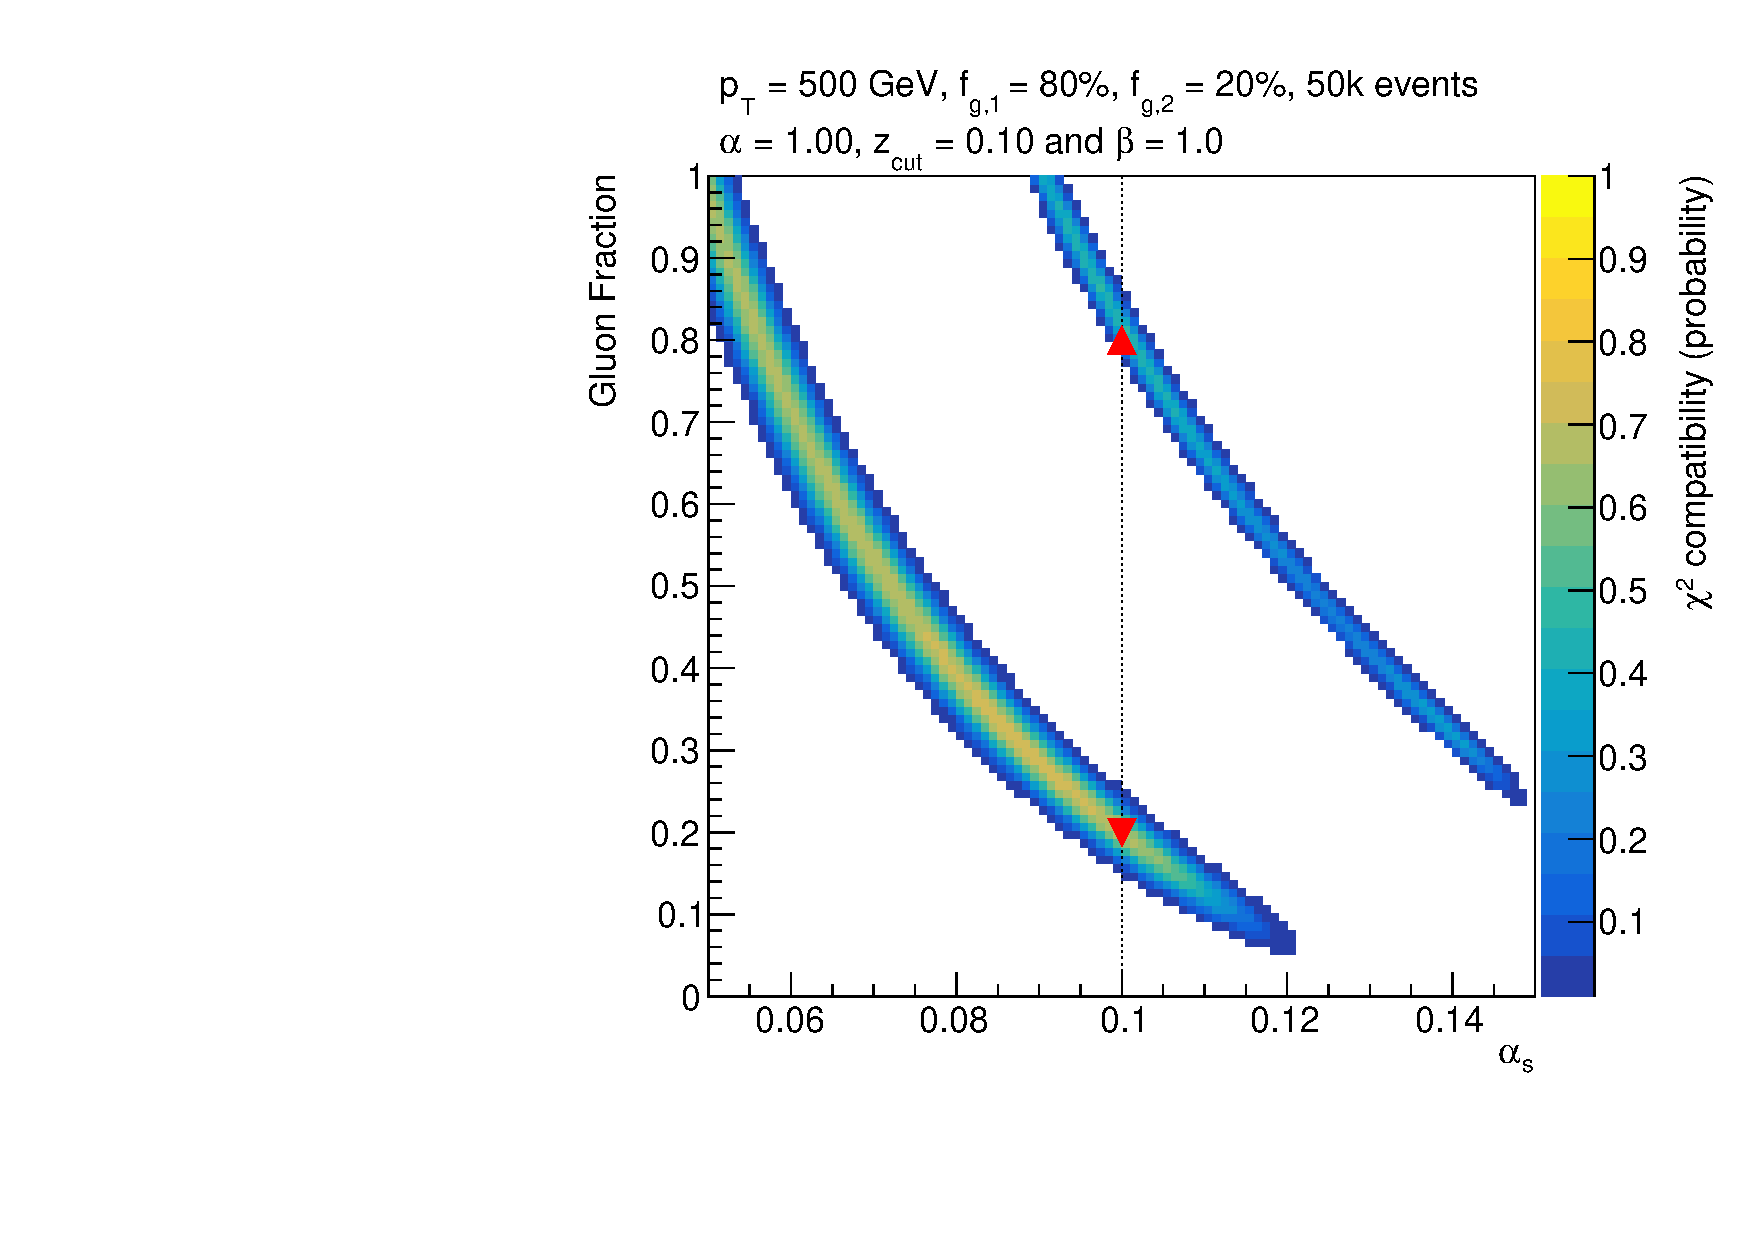
\includegraphics[width = 0.32\columnwidth]{jetsub_alphas_banana_alpha_10beta_10_zcut_123451324.pdf}
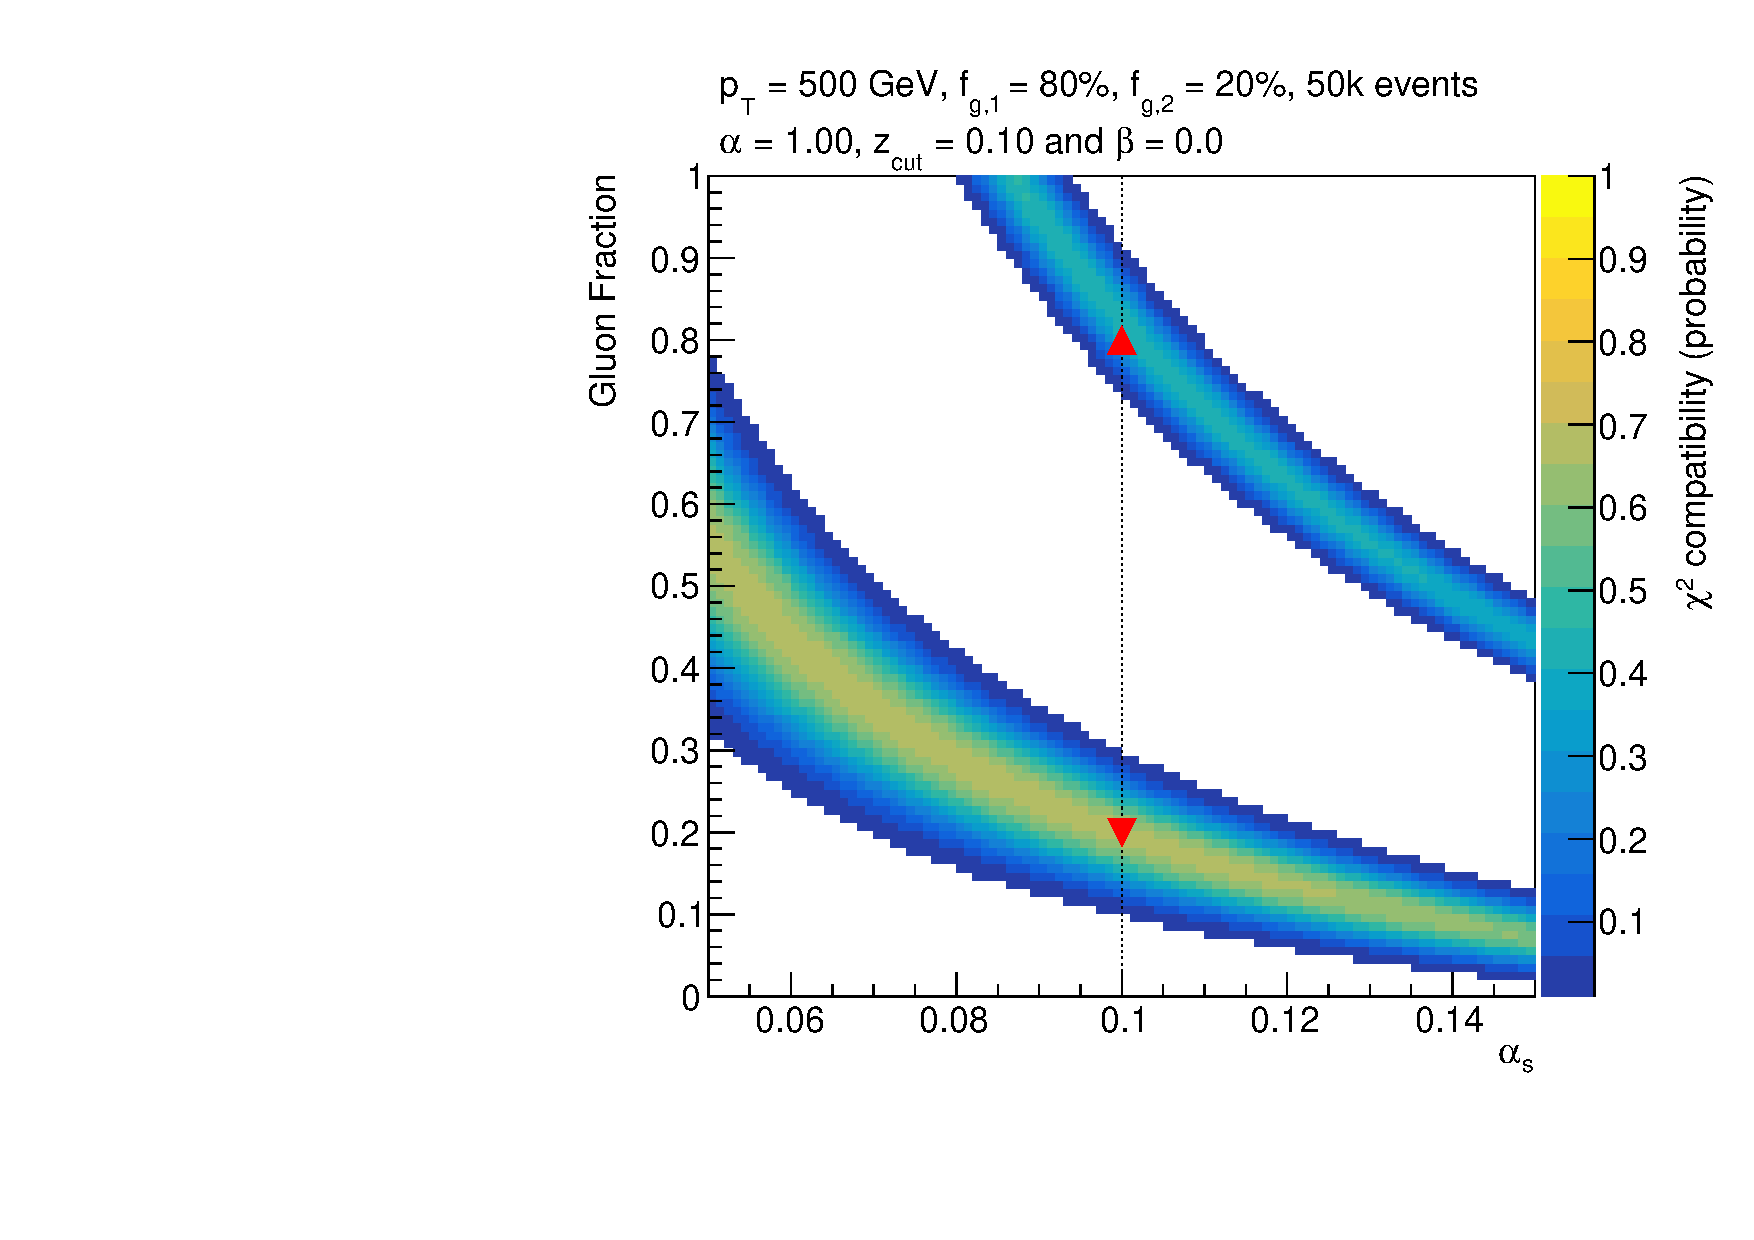
\includegraphics[width = 0.32\columnwidth]{jetsub_alphas_banana_alpha_10beta_0_zcut_123451324.pdf}
\end{center}
\caption{The same as the left plot of Fig.~\ref{jetsub_alphas_fig:alpha2fit}, but for the remaining three observables from Fig.~\ref{jetsub_alphas_fig:templates}.}
\label{jetsub_alphas_fig:morebananas}
\end{figure}


One way to improve the situation is to combine multiple $\alpha$, $\beta$, and $z_\mathrm{cut}$ values (only $\alpha$ and $\beta$ are varied here).
%
Figure~\ref{jetsub_alphas_fig:morebananas} shows the $f_g,\alpha_s$ fit for all of the $\alpha,\beta$ values from Fig.~\ref{jetsub_alphas_fig:templates} that were not shown in Fig.~\ref{jetsub_alphas_fig:alpha2fit}.
%
As in Fig.~\ref{jetsub_alphas_fig:alpha2fit}, there are two banana-shaped regions that correspond to the $f_g=20\%$ and $f_g=80\%$ samples.
%
The tilt of the bananas is slightly different than the $\alpha=2$, $\beta=0$ case and so there is a possibility to gain from combining the information in the observables.
%
In practice, a challenge with a multi-observable extraction strategy is the need to understand correlations between observables.
%
At the moment, joint distributions of two-point correlators are only known to NLL accuracy without grooming~\cite{Larkoski:2014pca}.

\begin{figure}[t]
\begin{center}
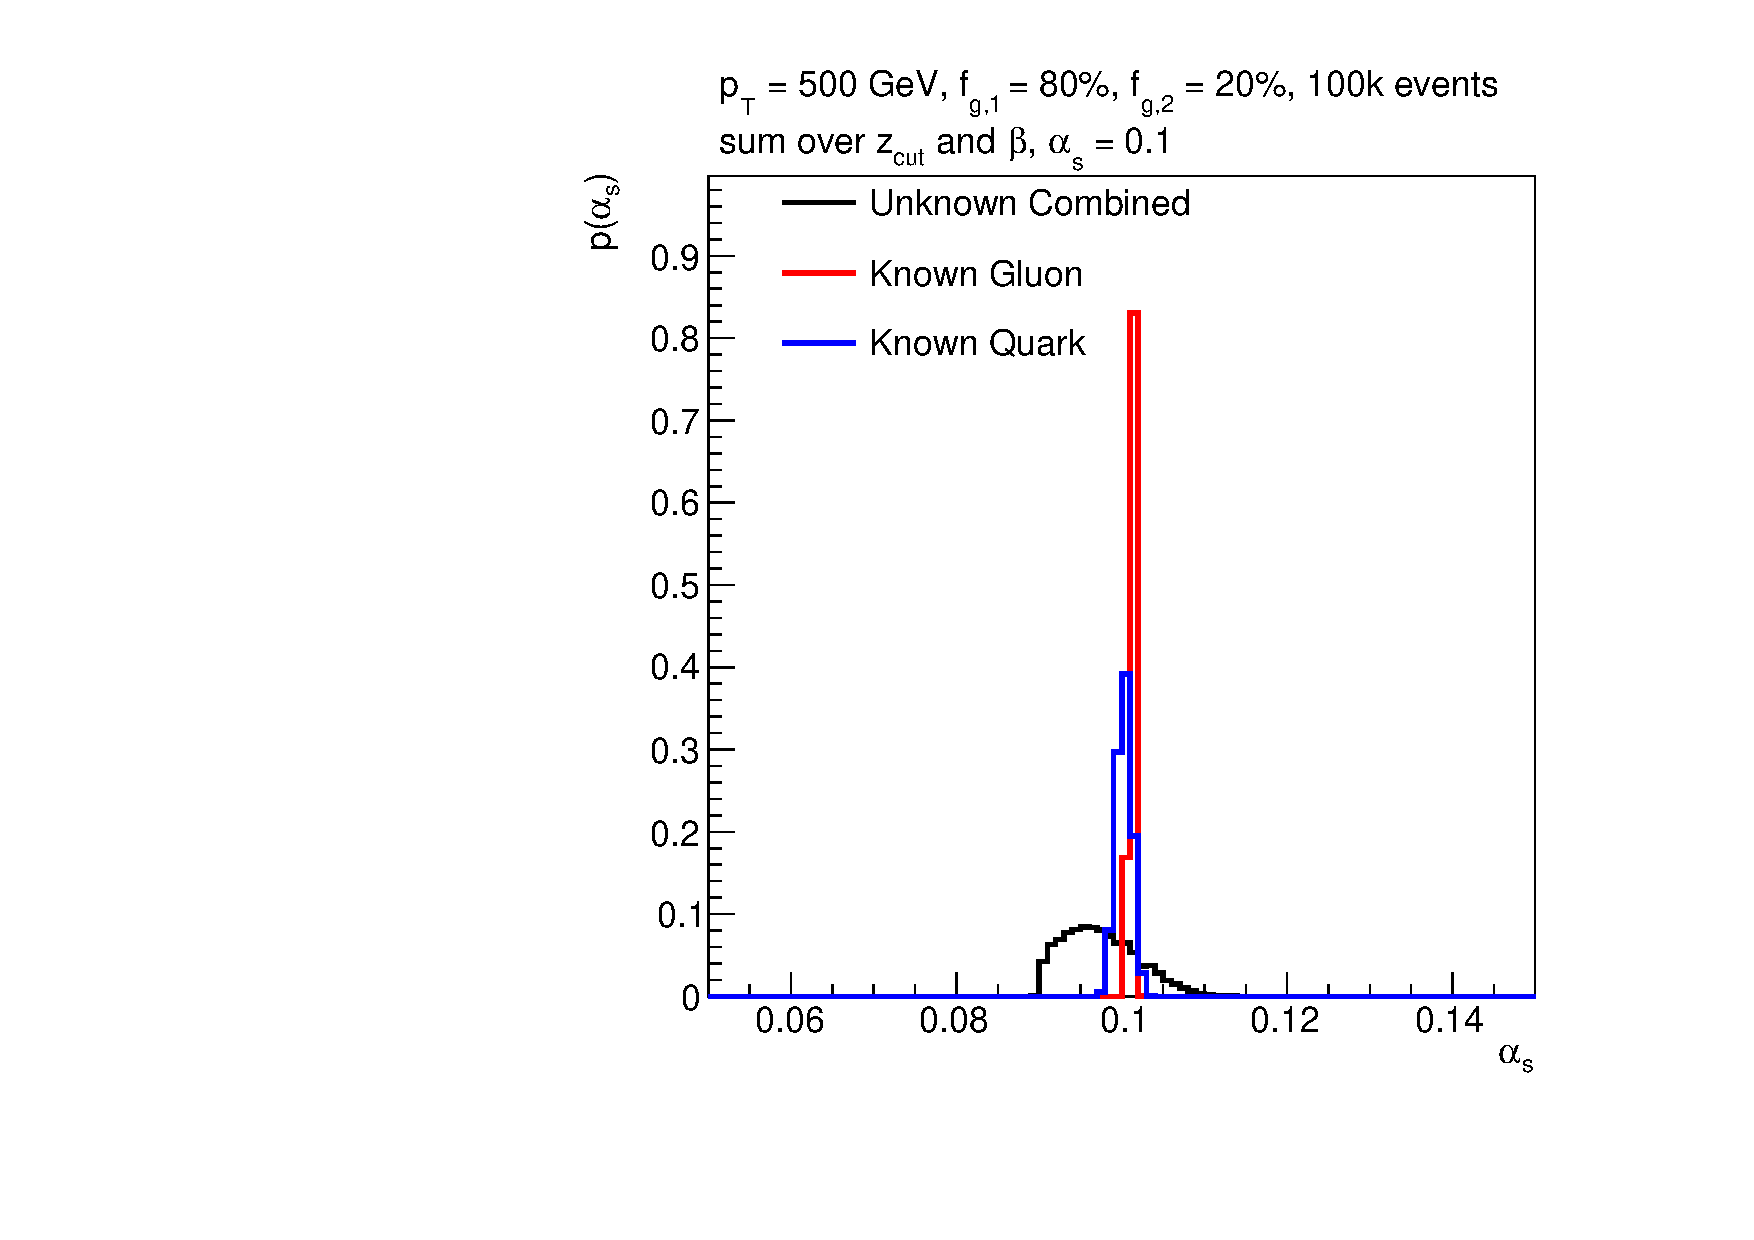
\includegraphics[width = 0.49\columnwidth]{jetsub_alphas_combination23451324.pdf}
\end{center}
\caption{Marginalizing the $f_g,\alpha_s$ fit over the gluon fraction for a fit that combines the four observables from Fig.~\ref{jetsub_alphas_fig:templates}.  The unknown combined mixture uses two samples with $f_g=20\%$ and $f_g=80\%$.}
\label{jetsub_alphas_fig:combo}
\end{figure}

With that caveat in mind, Figure~\ref{jetsub_alphas_fig:combo} shows the result of a combined fit assuming that all four distributions are statistically (and systematically) independent
%
This is a rather strong assumption that is unlikely to be even approximately true in practice.
%
However, the benefit of having different tilts in the $f_g,\alpha_s$ plane is clearly shown and would be a generic feature of a multi-observable fit, even if the size of the gain is not as significant as shown here.
%
It is important to emphasize that the black curve in Fig.~\ref{jetsub_alphas_fig:combo} assumes no prior knowledge of the gluon fraction of the event samples.
%
The fit can of course be improved by using some knowledge of the gluon fractions from the hard scattering process convolved with PDFs, as discussed in Sec.~\ref{subjetsub_alphas_sec:norm}.

\subsection{Estimate of Experimental Resolution}
\label{jetsub_alphas_sec:resolution}

To keep pace with precise theory predictions, the experimental resolution must be well-understood in order to ensure both precision and accuracy of jet substructure measurements.
%
To estimate the impact of detector resolution on $\alpha_s$ fit illustrated in Sec.~\ref{jetsub_alphas_sec:templates}, a fast simulation from \textsc{Delphes} 3.4.1~\cite{deFavereau:2013fsa} was studied using particle-level input from \textsc{Pythia~8}.210.
%
This setup uses a CMS-like detector with jets built from particle-flow objects.
%
There are generically two regimes for determining the experimental resolution.
%
At high mass, there are well-resolved hard prongs in the jet, so the resolution is set by the jet energy resolution of those ``sub-jets''.
%
At low mass, the groomed jet is defined by nearly collinear splittings at which point the angular resolution can dominate.


\begin{figure}[t]
\begin{center}
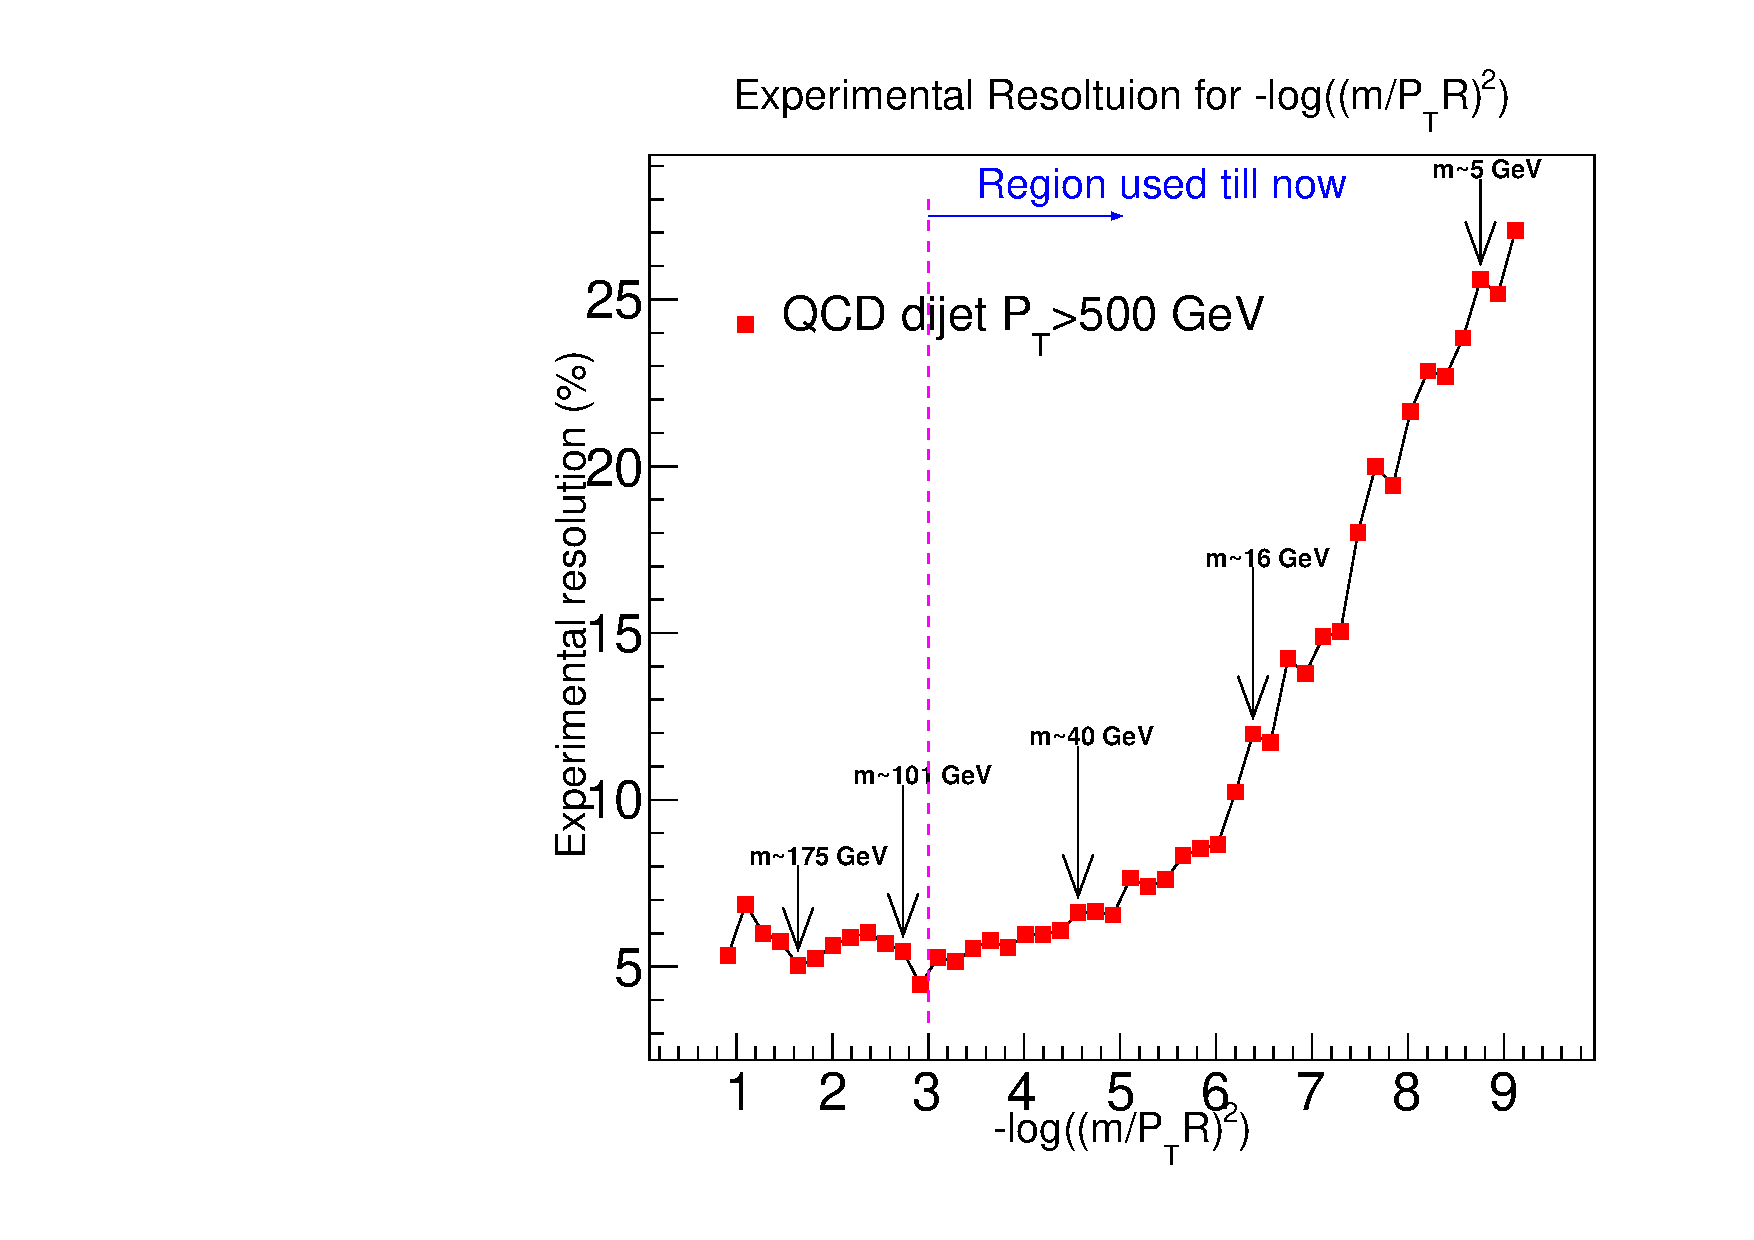
\includegraphics[width = 0.49\columnwidth]{jetsub_alphas_Resolution_plot_logrho_updated2.pdf}
\end{center}
\caption{The fractional $e_2^{(2)}$ distribution determined from dijet events simulated with \textsc{Pythia~8} plus \textsc{Delphes}.  Arrows indicate the mass at given values of the two-point correlator.  The upper bound of the resummation regime is indicated by a dashed line.  Larger masses are to the left.}
\label{jetsub_alphas_fig:resolution}
\end{figure}

\begin{figure}[t]
\begin{center}
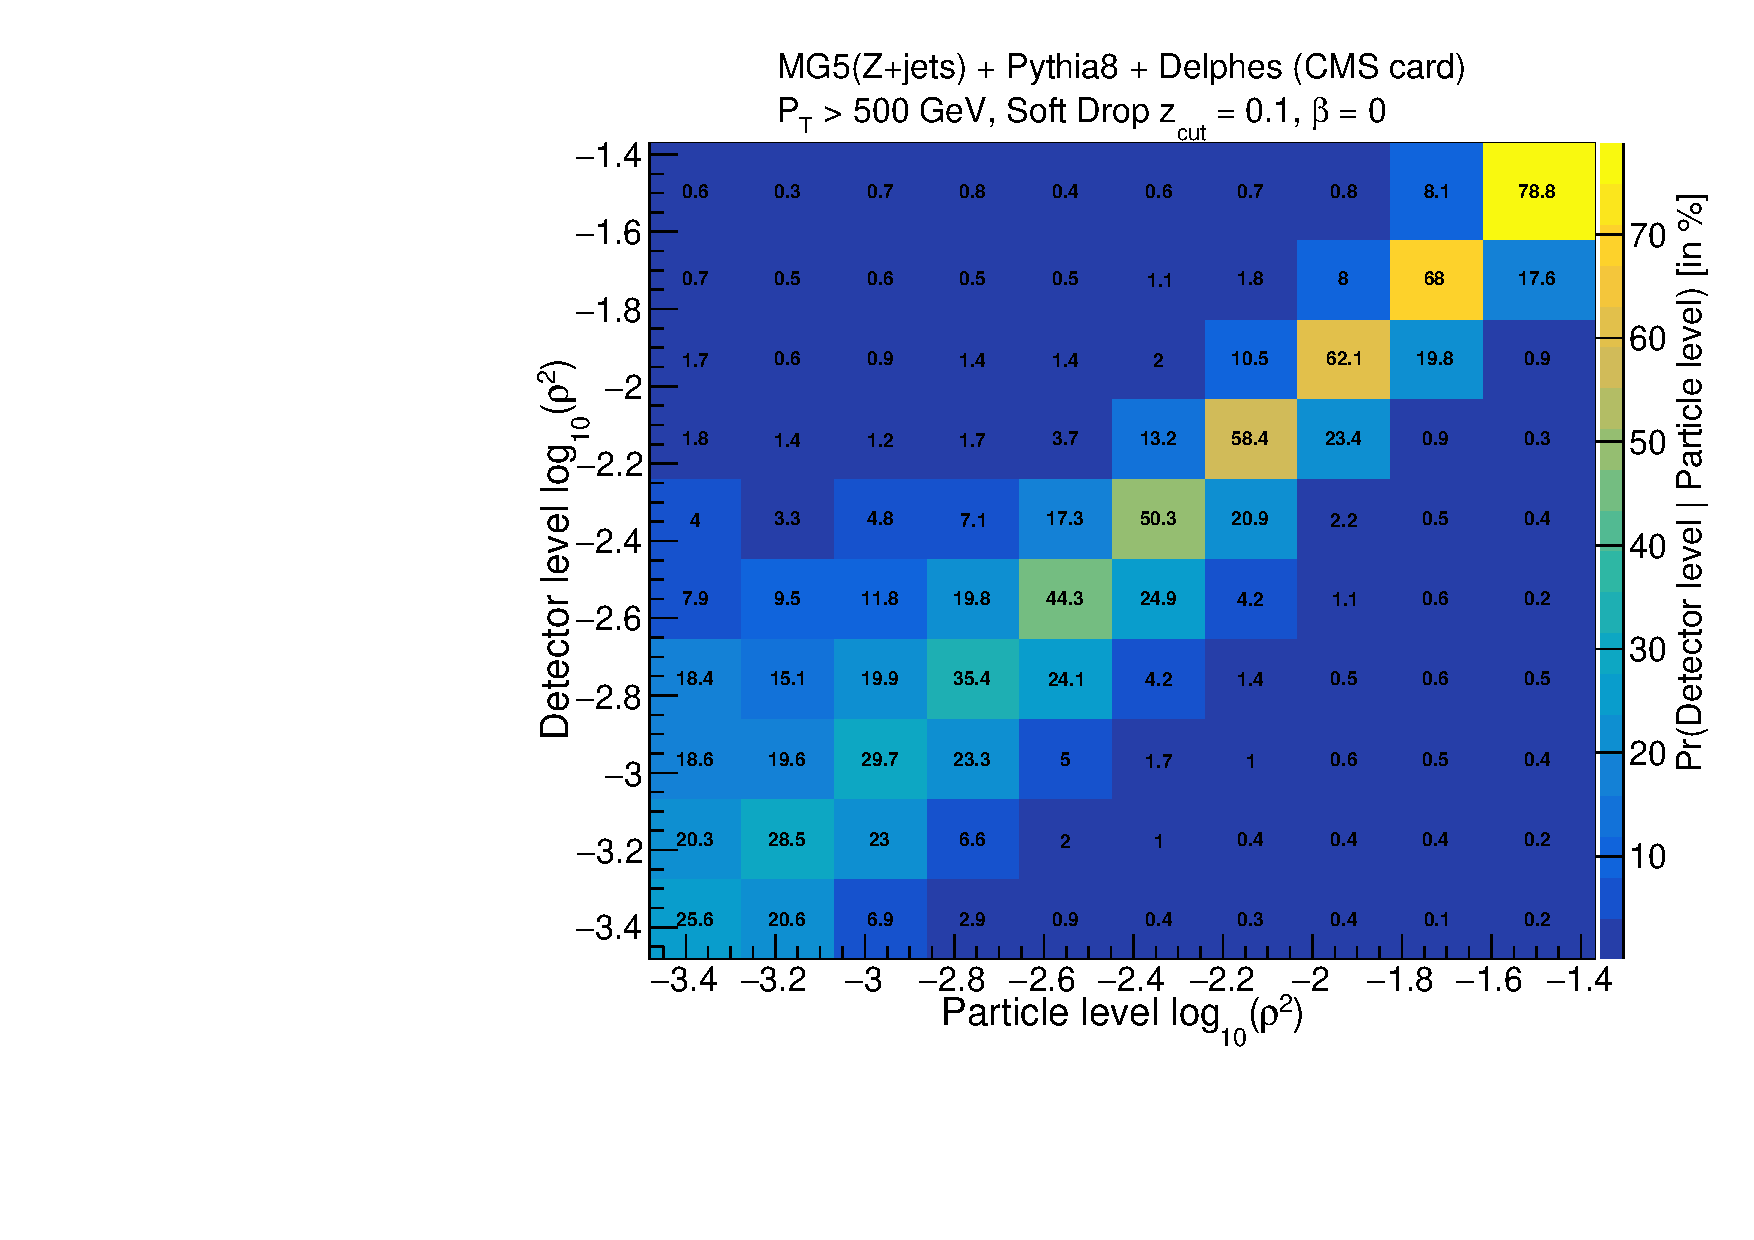
\includegraphics[width = 0.49\columnwidth]{jetsub_alphas_Rho_2D.pdf}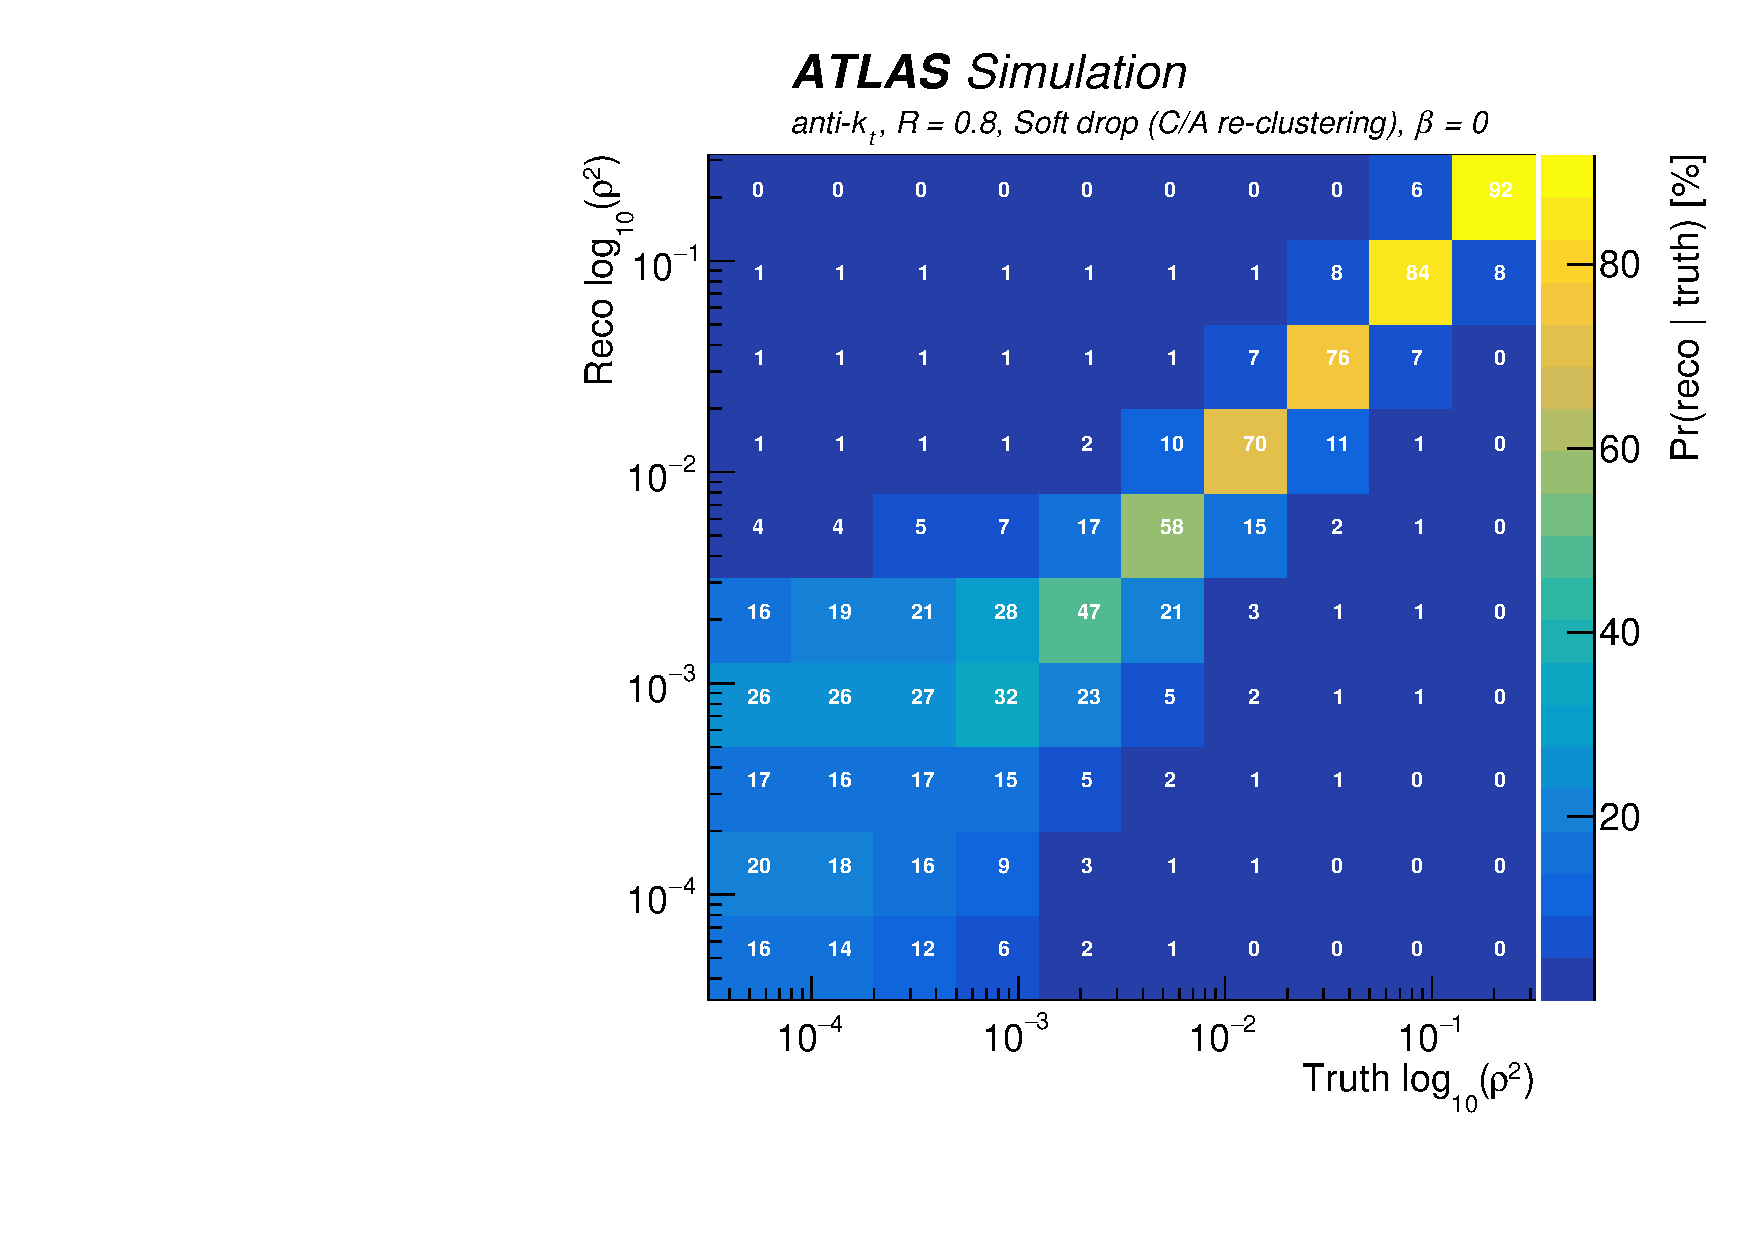
\includegraphics[width = 0.49\columnwidth]{jetsub_alphas_figaux_03a.pdf}
\end{center}
\caption{Left: The migration matrix between particle-level and detector-level using the Delphes simulation (left) and from the ATLAS measurement (right; reproduced from Ref.~\cite{Aaboud:2017qwh}).  Unlike previous plots, larger masses are on the right (shown this way to match the ATLAS result). }
\label{jetsub_alphas_fig:expres}
\end{figure}

Figure~\ref{jetsub_alphas_fig:resolution} shows the fractional $e_2^{(2)}$ resolution estimated from \textsc{Delphes}.
%
The resolution is smallest at high mass due to the excellent energy resolution of the CMS-like detector.
%
The resolution at low mass is about 10\% near 15 GeV and reaches 30\% near the limit of $\mathcal{O}(\mathrm{few GeV})$.
%
Encouragingly, the fits in Sec.~\ref{jetsub_alphas_sec:templates} relied only on the regime where $\sim 10\%$ resolution seems to be achievable, which gives an indication that a 10\% extraction of $\alpha_s$ should be feasible.
%
As a check that this estimated resolution is sensible, Fig.~\ref{jetsub_alphas_fig:expres} compares the migration matrix extracted from Delphes to the one published in the recent ATLAS measurement~\cite{Aaboud:2017qwh}.
%
Here, the comparison is between the particle-level and detector-level groomed mass values. 
%
The migration is qualitatively the same, with an excellent diagonal behavior (low migrations) at high mass and a worse resolution at low mass.






\begin{figure}[t]
\begin{center}
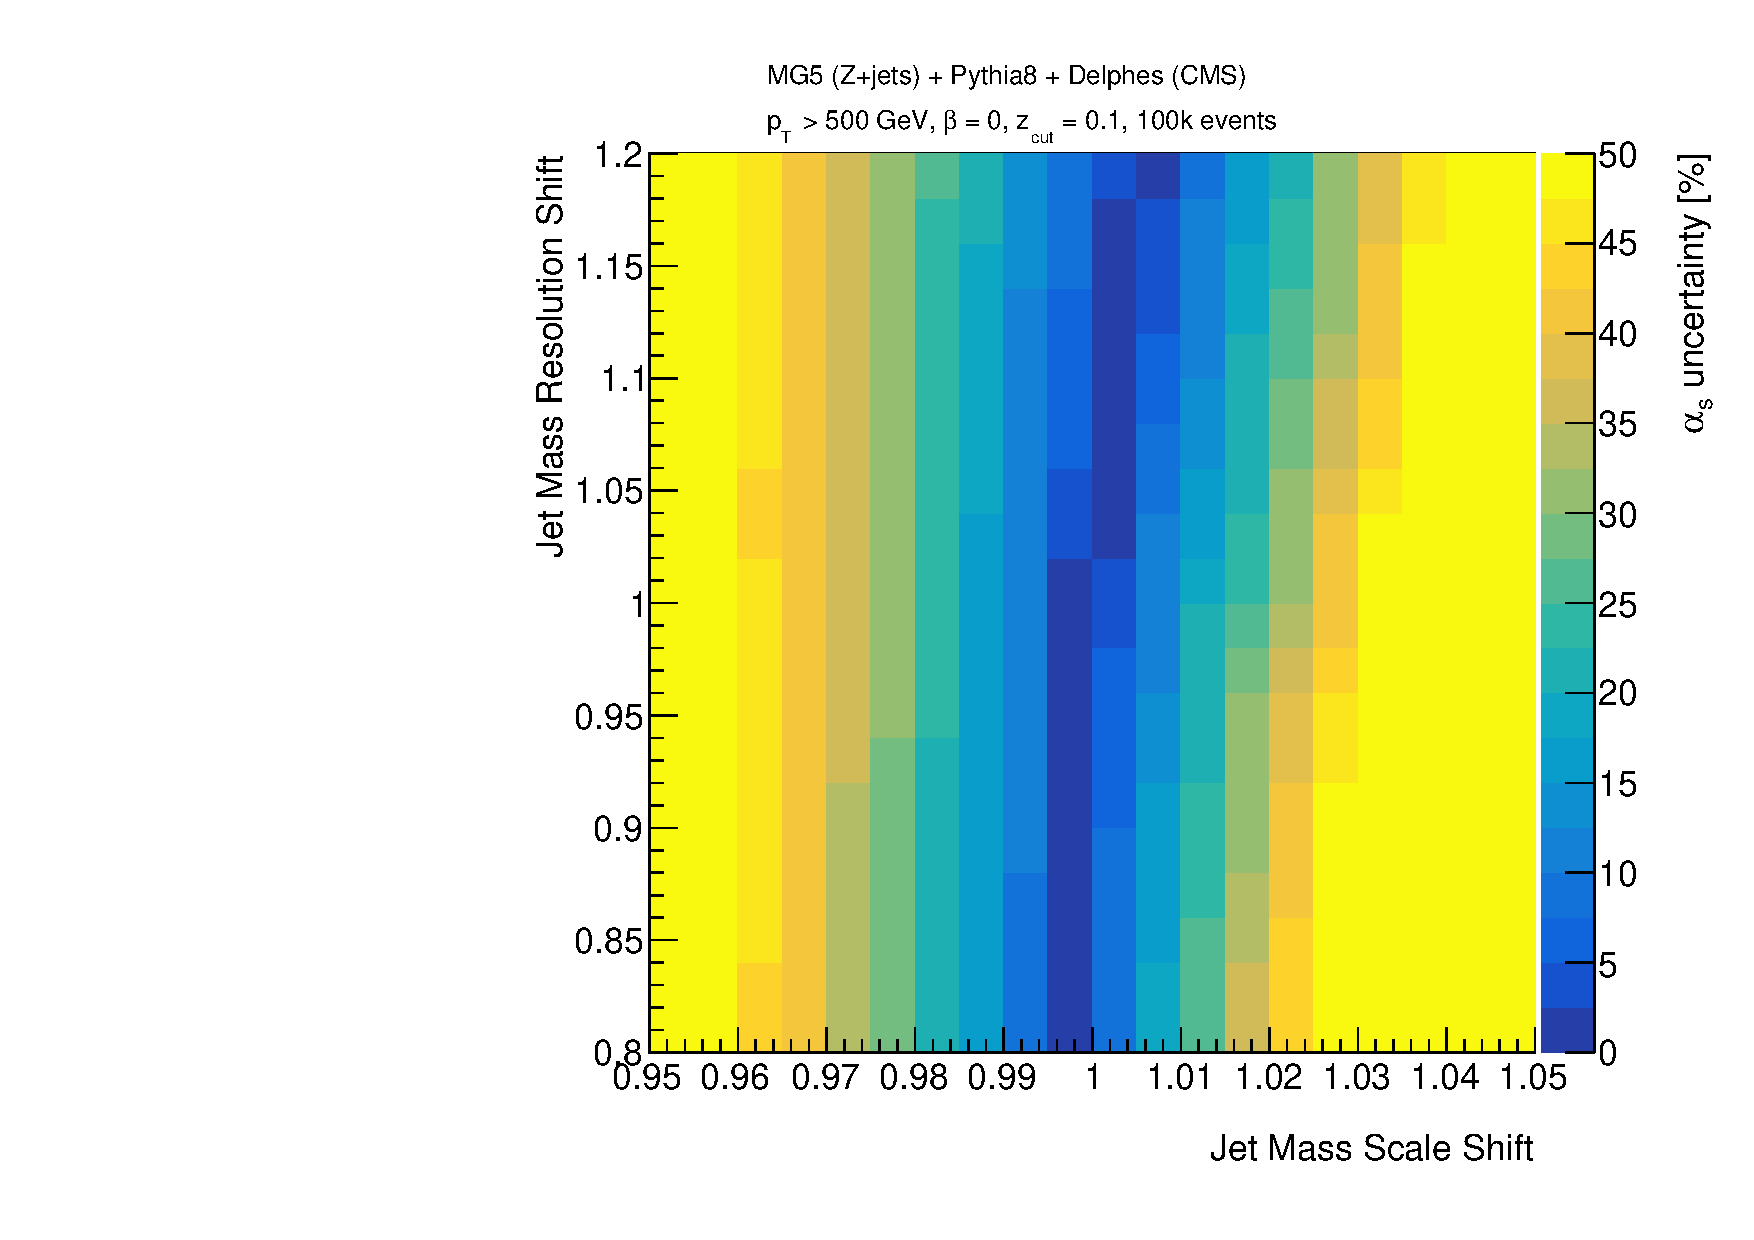
\includegraphics[width = 0.49\columnwidth]{jetsub_alphas_resolution_scan.pdf}
\end{center}
\caption{The impact of jet mass scale and jet mass resolution uncertainties on the uncertainty in the measured value of $\alpha_s$.  See the text for details.}
\label{jetsub_alphas_fig:expfit}
\end{figure}

To understand the sensitivity to jet mass scale and resolution uncertainties, we conduct pseudo-experiments by sampling from the templates described in Sec.~\ref{jetsub_alphas_sec:templates} and smearing with the migration matrix shown in the left plot of Fig.~\ref{jetsub_alphas_fig:expres}.
%
We then unfold with another migration matrix that has the jet mass scale shifted or smeared by a fixed amount, and extract $\alpha_s$ via Eq.~\ref{jetsub_alphas_eq:chi2fit} but for fixed and known $f_g=0$.
%
The results of this procedure are shown in Fig.~\ref{jetsub_alphas_fig:expfit}.
%
There is little sensitivity to the jet mass resolution while there is a large uncertainty in the extracted $\alpha_s$ if the uncertainty in the jet mass scale exceeds a few percent.
%
Current jet mass scale uncertainties are below $5\%$ and resolution uncertainties are below 20\%~\cite{ATLAS-CONF-2017-063,CMS-PAS-JME-16-003}.
%
The mass scale uncertainty is as small as $2\%$ in various regions of phase space.
%
This again suggests that a $\sim 10\%$ measurement of $\alpha_s$ is feasible, as the uncertainty on the jet mass scale reaches the same level of maturity as the jet energy scale over the next few years.

\section{Conclusions and Future Outlook}
\label{jetsub_alphas_sec:future}

In this paper, we performed a preliminary study assessing a possible extraction of the strong coupling constant $\alpha_s$ from groomed jet substructure measurements at the LHC.
%
This has been made possible by recent advances in the calculation of groomed event shapes, which allow them to be resummed to NNLL accuracy, as well as advances in the understanding of the experimental uncertainties for groomed jet observables.
 
We have highlighted a number of features that an extraction of $\alpha_s$ from groomed substructure would offer.
%
In particular, the grooming procedure suppresses NP hadronization corrections to the mass distribution, extending the range of perturbative control by up to a factor of $\sim 100$ as compared to the ungroomed case, where hadronization corrections are a dominant uncertainty.
%
Furthermore, the nature of the NP corrections is completely different, and therefore a groomed extraction could provide complementary information to event shape measurements at LEP and other $e^+e^-$ colliders. 

Using the groomed jet mass as a concrete example, we performed a feasibility study for the extraction of $\alpha_s$ from groomed jet substructure.
%
Considered separately, the groomed quark and gluon distributions both exhibit good sensitivity to $\alpha_s$.
%
However, this study also highlighted a key issue relevant at the LHC.
%
The leading behavior of the shape of the distribution is sensitive to the product $\alpha_s C_i$, where $C_i$ is the color Casimir factor, namely $C_A$ for gluon jets and $C_F$ for quark jets.
%
This immediately implies that there is a degeneracy between the value of $\alpha_s$ and the quark/gluon fraction of the sample.
%
We highlighted two possible ways of overcoming this degeneracy, either by a fixed-order calculation of the quark and gluon fractions, or by a simultaneous measurement of different substructure observables.
%
This would ideally be combined with multiple samples with (relatively pure~\cite{Gallicchio:2011xc}) quark/gluon fractions.
%
While we expect significantly better precision to be achievable by the explicit calculation, this would introduce a stronger dependence on the PDFs which then should ideally be fitted simultaneously.

With currently achievable experimental and theoretical uncertainties, we have shown that an extraction of $\alpha_s$ at the $10\%$ level is realistic using the currently available data at the LHC.
%
We believe that this study motivates a serious effort to extract the strong coupling constant $\alpha_s$ from jet substructure at the LHC using groomed jet shapes.
%
A serious analysis will require advances on both the theory and experiment sides, so we conclude by discussing some of the major obstacles that must be overcome.

On the theory side, we can separately discuss three primary aspects of the calculation:
%
\begin{itemize}
\item {\bf Resummation Accuracy:} For $e^+e^-$ event shapes, the current state of the art is N$^3$LL.
%
This has been achieved only for a few select observables using soft-collinear effective theory.
%
The extension to N$^3$LL accuracy for the groomed jet mass would require only the calculation of the anomalous dimensions for the groomed soft function to three loops, which is possible using currently available techniques.
%
At this level of accuracy, it will also be important to asses perturbative power corrections in $z_{\mathrm{cut}}$.
%
While \cite{Marzani:2017kqd,Marzani:2017mva} have shown that these corrections are numerically small, they may become important if multiple $z_{\mathrm{cut}}$ values are used that are not much less than one.
%
\item {\bf Fixed-Order Matching:} A key aspect, and a potential complication to achieve theoretical accuracy competitive with $e^+e^-$ determinations, is fixed-order matching.
%
For $e^+e^-$, the perturbative corrections to $e^+e^- \rightarrow$ 3 jets are known to NNLO \cite{GehrmannDeRidder:2007hr,Gehrmann-DeRidder:2007nzq,Weinzierl:2008iv,Weinzierl:2009ms}.
%
To achieve a similar perturbative accuracy for the matching for the groomed jet mass will require $2\rightarrow 3$ matrix elements at NNLO.
%
While results for the amplitudes are just becoming available \cite{Gehrmann:2015bfy,Dunbar:2016aux,Badger:2013yda,Badger:2017jhb,Abreu:2017hqn}, it will be a while before numerically-efficient evaluations of the relevant cross-sections are available.
%
We believe that this is currently the theoretically most difficult ingredient.
%
\item {\bf Non-Perturbative Corrections:} Finally, in addition to improving our understanding of the perturbative accuracy of the observable, it will also be crucial to improve our understanding of the NP aspects of groomed observables.
%
While it has been shown through PS studies that NP effects are suppressed throughout a large component of the distribution, it will be important to quantify this further.
%
In the case of $e^+e^-$ event shapes, operator definitions of soft matrix elements allow for field theoretic definitions of the NP parameters.
%
Ideally this could also be performed for groomed observables, placing the groomed jet mass on a firmer theoretical footing.
%
\end{itemize}

Experimentally, there are three broad topics that need to be addressed for a precision extraction of $\alpha_s$:
%
\begin{itemize}
%
\item {\bf Mass Scale Uncertainties:} At the moment, ATLAS~\cite{Aaboud:2017qwh} and CMS~\cite{CMS-PAS-SMP-16-010} have very different approaches for determining the jet mass scale uncertainty, both with known limitations.
%
CMS performs a fit to the hadronic $W$ boson mass peak in one-lepton $t\bar{t}$ events and takes the shift in the peak position as the uncertainty in the jet mass scale (which is negligible and thus ignored)~\cite{Sirunyan:2016cao}.
%
Two challenges with this approach are that (a) the peak position is a convolution of particle-level and detector-level effects and (b) it is not clear that uncertainties derived for boosted $W$ bosons should be the same as for generic quark and gluon jets at all masses.
%
One can overcome (a) with a technique like forward-folding~\cite{ATLAS-CONF-2016-008,ATLAS-CONF-2016-035}.
%
Various PS generators can be studied, but it is likely not sufficient to have one global model comparison.
%
The impact on the jet mass resolution in one topology may be completely different than the impact of the scale, resolution, or acceptance in another topology.

By contrast, the ATLAS measurement propagates constituent-based uncertainties through to the groomed mass.
%
These uncertainties are derived from matching tracks to calorimeter-cell clusters and studying the energy and angular matching.
%
Studies have shown that this ``bottom-up'' approach works well for reproducing the jet energy scale~\cite{Aaboud:2016hwh}, which has been validated also for groomed jets in \cite{Aaboud:2017qwh}.
%
However, this does not hold exactly for the mass, which is not linear in the constituent energies~\cite{Nachman:2016qyc}.
%
The uncertainties are validated using the standard ATLAS approach using track-jets~\cite{Aad:2013gja,ATLAS-CONF-2017-063}, but to achieve higher precision, a more detailed understanding of the impact of energy thresholds, fluctuation correlations, and calorimeter cluster merging will be required.
%
\item {\bf Mass Resolution Uncertainties:} ATLAS and CMS use their same respective approaches for the mass resolution as for the mass scale (i.e.\ bottom-up and $W$ mass peak).
%
ATLAS validates their approach in a similar manner as CMS, by using the $W$ mass peak from $t\bar{t}$ events.%
\footnote{This validation does not have the same complete forward-folding machinery as was used by ATLAS for trimmed jets.}
%
From \cite{jetsub_alphas_fig:expfit}, it seems that the mass resolution will not be the limiting factor, but it could be if the situation is not improved as the jet mass scale precision improves.
%
\item {\bf Pileup Modeling and Mitigation:} Grooming significantly reduces the impact of pileup, but if the Run 3+ data are to be used (pileup levels of 80+), then a significantly better and more detailed understanding of the degradation due to pileup will be required.
%
Statistical uncertainties are currently not dominant, so it is conceivable that the higher instantaneous luminosity data will not be required for the precision $\alpha_s$ extraction.
%
This may change if one wants to exploit the largest lever-arm possible; to access the highest $p_{\mathrm{T}}$ jets, we will need more data.
%
\end{itemize}

We are optimistic that these difficulties on both the theory and experiment side can be overcome, enabling a precision probe of the strong coupling constant from jet substructure in the LHC environment.
%
We also hope that this study motivates additional investigations to broaden the potential toolbox for $\alpha_s$ extraction.
%
At minimum, it would be interesting to study in more detail the use of other observables beyond the two-point correlators as well as alternative grooming techniques beyond mMDT/Soft Drop.
%
More ambitiously, one potentially interesting direction is the use of track-based measurements, since it may be the case that it is ultimately experimental uncertainties that are the limiting factor.
%
From the experimental perspective, this significantly reduces uncertainties, particularly in a high pile-up environment.
%
From the theoretical side, however, it introduces the need for NP track functions.
%
That said, only certain moments of the track functions are required for special observables, and it may be possible to perform a combined fits for the moments of the track functions and $\alpha_s$, much like how fits are performed for $e^+e^-$ event shapes.
%
Significantly more theoretical work is required to see if this is truly a viable possibility, although we believe that this is well motivated.


\section*{Acknowledgments}

The work of GS is supported in part by the French Agence Nationale de la Recherche,
under grant ANR-15-CE31-0016, and by the ERC Advanced Grant Higgs@LHC
(No.\ 321133).
%
The work of FD and JT is supported by the DOE under grant contract numbers DE-SC-00012567 and DE-SC-00015476.
%
IM and BN are supported in part by the Office of High Energy Physics of the U.S. Department of Energy under Contract No. DE-AC02-05CH11231, and the LDRD Program of LBNL.

\bibliography{lh2017_alphas}

\end{document}
